% !TEX encoding = UTF-8 Unicode
% !TEX TS-program = xelatex
\documentclass[12pt]{article}
\usepackage{tikz}
\usepackage{pgfplots}
\usetikzlibrary{calc, arrows, patterns,angles ,positioning,quotes}
\usetikzlibrary{decorations.markings}
\usetikzlibrary{arrows.meta}

\usepackage{tkz-euclide}
%\usepackage{tkz-euclide}
%\usetkzobj{all}

%==== Chinese Setting  ====== 

\input{E:/NCTUG2/TEX/LatexCodeTemplate/inputFile/Qheader.tex}

\begin{document}
    
    
    

    
\begin{tikzpicture}[x={(-0.8cm,-0.7cm)},y={(1.3 cm, 0cm)},z={(0cm,0.2cm)}]                
\coordinate (xStart) at (0,0,0);
\coordinate (xEnd) at (10,0,0);
\coordinate (yStart) at (0,0,0);
\coordinate (yEnd) at (0,6,0);
\coordinate (zStart) at (0,0,0);
\coordinate (zEnd) at (0,0,8);

\draw[-{Stealth[scale=1.3,angle'=45]},semithick]  (xStart) --(xEnd) ;
\coordinate (A) at (1,-4,3);
\coordinate (B) at (7, 6,8);
\coordinate (AP) at (1,0,0);
\coordinate (BP) at (7,0,0);
\coordinate (P) at (3,0,0);

\draw [draw=black, every edge/.append style={draw=black, dashed}]
(A) -- (P)
(B) -- (P);

\draw [draw=black, every edge/.append style={draw=black, dashed}]
(A) edge node[midway, above] {$5$} (AP) ;
 

\draw [draw=black, every edge/.append style={draw=black, dashed}]
(B) edge node[midway, below]{$10$} (BP);

\node[] at ($(AP)!0.5!(P)$) {$\textc{1}$};
\node[] at ($(BP)!0.5!(P)$) {$\textc{2}$};

\foreach \v/\u/\t in 
{A/180/$A$,
    P/180/$P$,
    B/0/$B$
}
{
    \draw[ultra thick,fill] (\v) circle (2pt);
    \node[label=\u:\t] at (\v){};
};     
    
    \draw[ultra thick,fill] (AP) circle (2pt);
    \node[] at (AP){$A^\prime$};
    \draw[ultra thick,fill] (BP) circle (2pt);
    \node[left] at (BP){$B^\prime$};
    \tkzMark[size=0.3](B,BP,P)
    \tkzMark[size=0.3](A,AP,P)
    \node[below left ] at (xEnd) {$x$};
    \node[below] at (P){$\times$};
    \node[above] at (P){$\times$};
    
\end{tikzpicture}    
    
%       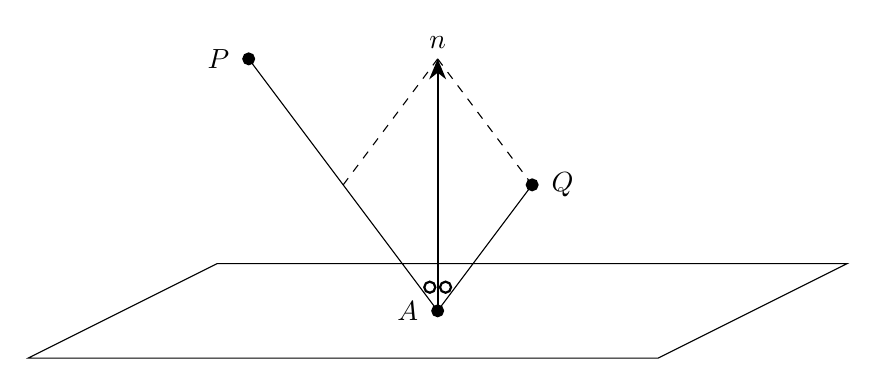
\begin{tikzpicture}[x={(-0.4cm,-0.2cm)},y={(1 cm, 0cm)},z={(0cm,1cm)}]
        \coordinate (A) at (0,0,0);
        \coordinate (R) at (3, 4,0);
        \coordinate (S) at (-3,4,0);
        \coordinate (T) at (-3,-4,0);
        \coordinate (U) at (3,-4,0);
        
        \coordinate (P) at (0,-2.4 ,3.2);
        \coordinate (M) at ($(P)!0.5!(A)$); 
        \coordinate (Q) at (0, 1.2 ,1.6);
        
        \coordinate (x) at (3.5,0,0);
        \coordinate (y) at (0,3,0);
        \coordinate (z) at (0,0,3);
        \coordinate (n) at (0,0,3.2);
        \draw [draw=black, every edge/.append style={draw=black, dashed}]
        (R) -- (S) --(T) -- (U) -- cycle
        (P) -- (A)
        (A) -- (Q)
        (M) edge (n)
        (n) edge (Q)
        ;
        \draw[-{Stealth[scale=1.3,angle'=45]},semithick] (A) -- (n) node[above] {$\lvec{n}$};
        \draw[thick] (0,0.1,0.3) circle (2pt);
        \draw[thick] (0,-0.1,0.3) circle (2pt);
        
        
        \foreach \v/\u/\t in 
        {A/180/$A$,
            P/180/$P$,
            Q/0/$Q$
        }
        {
            \draw[ultra thick,fill] (\v) circle (1.5pt);
            \node[label=\u:\t] at (\v){};
        };     
        \end{tikzpicture}
        
    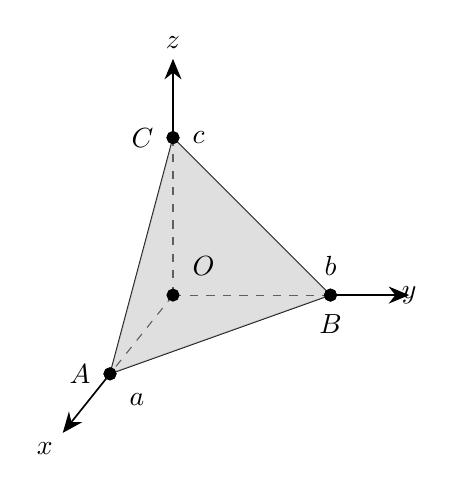
\begin{tikzpicture}[x={(-0.4cm,-0.5cm)},y={(1 cm, 0cm)},z={(0cm,1cm)}]
    \coordinate (O) at (0,0,0);
    \coordinate (A) at (2, 0,0);
    \coordinate (B) at (0,2,0);
    \coordinate (C) at (0,0,2);
    \coordinate (x) at (3.5,0,0);
    \coordinate (y) at (0,3,0);
    \coordinate (z) at (0,0,3);
    \draw [draw=black, every edge/.append style={draw=black, dashed}]
    (A) -- (B) --(C) --cycle
    (O) edge (A)
    (O) edge (B)
    (O) edge (C);
    
    \draw[-{Stealth[scale=1.3,angle'=45]},semithick] (A) -- (x) node[below left] {$x$};
    \draw[-{Stealth[scale=1.3,angle'=45]},semithick] (B) -- (y) node[] {$y$};
    \draw[-{Stealth[scale=1.3,angle'=45]},semithick] (C) -- (z) node[above] {$z$};
    \fill [lightgray, opacity=0.5] (A) -- (B) -- (C)-- cycle;
    
    \foreach \v/\u/\t in 
    {A/180/$A$,
        B/270/$B$,
        C/180/$C$,
        A/315/$a$,
        B/90/$b$,
        C/0/$c$,
        O/45/$O$
    }
    {
        \draw[ultra thick,fill] (\v) circle (1.5pt);
        \node[label=\u:\t] at (\v){};
    };     
    \end{tikzpicture}
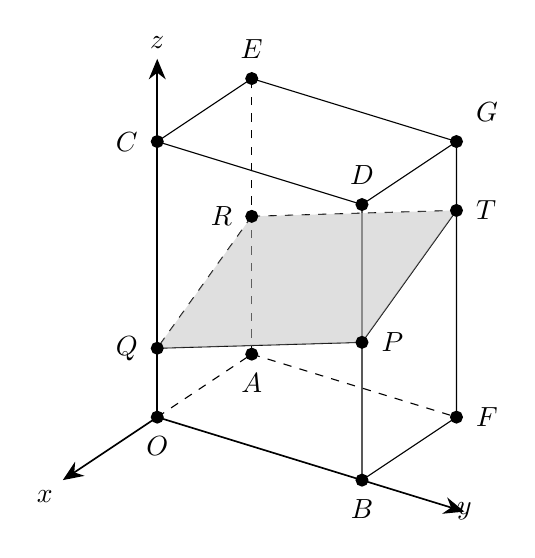
\begin{tikzpicture}[x={(-1.2cm,-0.8cm)},y={(1.3 cm,-0.4cm)},z={(0cm,3.5cm)}]
\coordinate (O) at (0,0,0);
\coordinate (B) at (0,2,0);
\coordinate (C) at (0,0,1);
\coordinate (A) at (-1, 0,0);
\coordinate (F) at (-1,2,0);
\coordinate (D) at (0,2,1);
\coordinate (G) at (-1,2,1);
\coordinate (E) at (-1,0,1);
\coordinate (x) at (1,0,0);
\coordinate (y) at (0,3,0);
\coordinate (z) at (0,0,1.3);
\coordinate (P) at ($(D)!0.5!(B)$);
\coordinate (Q) at ($(O)!0.25!(C)$);
\coordinate (R) at ($(A)!0.5!(E)$);
\coordinate (T) at (-1,2,0.75);
      \draw [draw=black, every edge/.append style={draw=black, dashed}]
      (C) -- (D) --(G) -- (E) --cycle
      (O) edge (A)
      (A) edge (F)
      (A) edge (E)
      (R) edge (T)
      (R) edge (Q)
      (P) -- (Q)
      (P) -- (T)
      (D) -- (B)
      (G) -- (F)
      (B) -- (F);

\draw[-{Stealth[scale=1.3,angle'=45]},semithick] (O) -- (x) node[below left] {$x$};
\draw[-{Stealth[scale=1.3,angle'=45]},semithick] (O) -- (y) node[] {$y$};
\draw[-{Stealth[scale=1.3,angle'=45]},semithick] (O) -- (z) node[above] {$z$};
        \fill [lightgray, opacity=0.5] (P) -- (Q) -- (R) -- (T) -- cycle;
        
        \foreach \v/\u/\t in 
        {A/270/$A$,
            B/270/$B$,
            C/180/$C$,
            D/90/$D$,
            E/90/$E$,
            F/0/$F$,
            G/45/$G$,
            R/180/$R$,
            Q/180/$Q$,
            P/0/$P$,
            T/0/$T$,
            O/270/$O$
        }
        {
            \draw[ultra thick,fill] (\v) circle (1.5pt);
            \node[label=\u:\t] at (\v){};
        };     
\end{tikzpicture}

        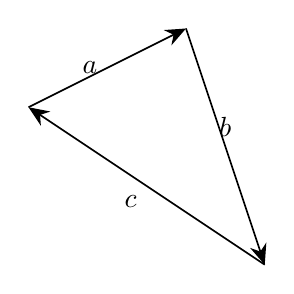
\begin{tikzpicture}
            \coordinate (A) at (0,0);
            \coordinate (B) at (2,1);
            \coordinate (C) at (3,-2);
            \draw[-{Stealth[scale=1.3,angle'=45]},semithick] (A) -- (B) node [midway, left]{$\lvec{a}$};
            \draw[-{Stealth[scale=1.3,angle'=45]},semithick] (B) -- (C) node [midway,above  ]{$\lvec{b}$};
            \draw[-{Stealth[scale=1.3,angle'=45]},semithick] (C) -- (A) node [midway,below left ]{$\lvec{c}$};
        \end{tikzpicture}
        
        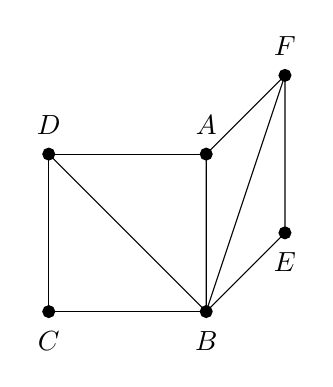
\begin{tikzpicture}
            \coordinate (A) at (0,0);
            \coordinate (B) at (0,-2);
            \coordinate (C) at (-2,-2);
            \coordinate (D) at (-2,0);
            \coordinate (E) at (1,-1);
            \coordinate (F) at (1,1);
            
            \draw (A) -- (B) -- (C) -- (D) -- cycle;
            
            \draw (A) -- (B) -- (E) -- (F) -- cycle;
            
            \draw (B) -- (D) 
                  (B) -- (F);
            \foreach \v/\u/\t in 
            {A/90/$A$,
             B/270/$B$,
             C/270/$C$,
             D/90/$D$,
             E/270/$E$,
             F/90/$F$
            }
            {
                \draw[ultra thick,fill] (\v) circle (1.5pt);
                \node[label=\u:\t] at (\v){};
            };     
            \tkzMark(D,A,B)
            \tkzMark(B,A,F)
        \end{tikzpicture}
        
        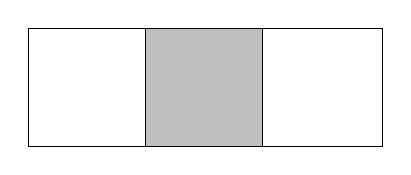
\begin{tikzpicture}[scale=0.5]
        \coordinate (A) at (0,0);
        \coordinate (B) at (9,0);
        \coordinate (C) at (9,-3);
        \coordinate (D) at (0,-3);       
        \coordinate (R) at ($(A)!0.33!(B)$);
        \coordinate (S) at ($(A)!0.66!(B)$);
        \coordinate (T) at ($(D)!0.33!(C)$);
        \coordinate (V) at ($(D)!0.66!(C)$);
        
        \draw (A) -- (B) -- (C) -- (D) -- cycle;
        \draw[fill=lightgray] (R) -- (S) -- (V) -- (T) -- cycle;
        \end{tikzpicture} 
        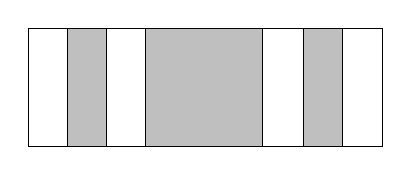
\begin{tikzpicture}[scale=0.5]
        \coordinate (A) at (0,0);
        \coordinate (B) at (9,0);
        \coordinate (C) at (9,-3);
        \coordinate (D) at (0,-3);       
        \coordinate (R) at ($(A)!0.33!(B)$);
        \coordinate (S) at ($(A)!0.66!(B)$);
        \coordinate (T) at ($(D)!0.33!(C)$);
        \coordinate (V) at ($(D)!0.66!(C)$);
        
        \draw (A) -- (B) -- (C) -- (D) -- cycle;
        \draw[fill=lightgray] (R) -- (S) -- (V) -- (T) -- cycle;
        
        \coordinate (A) at (0,0);
        \coordinate (B) at (3,0);
        \coordinate (C) at (3,-3);
        \coordinate (D) at (0,-3);       
        \coordinate (R) at ($(A)!0.33!(B)$);
        \coordinate (S) at ($(A)!0.66!(B)$);
        \coordinate (T) at ($(D)!0.33!(C)$);
        \coordinate (V) at ($(D)!0.66!(C)$);
        
        \draw[fill=lightgray] (R) -- (S) -- (V) -- (T) -- cycle;
        
        \coordinate (A) at (6,0);
        \coordinate (B) at (9,0);
        \coordinate (C) at (9,-3);
        \coordinate (D) at (6,-3);       
        \coordinate (R) at ($(A)!0.33!(B)$);
        \coordinate (S) at ($(A)!0.66!(B)$);
        \coordinate (T) at ($(D)!0.33!(C)$);
        \coordinate (V) at ($(D)!0.66!(C)$);
        
        \draw[fill=lightgray] (R) -- (S) -- (V) -- (T) -- cycle;
        \end{tikzpicture} 
        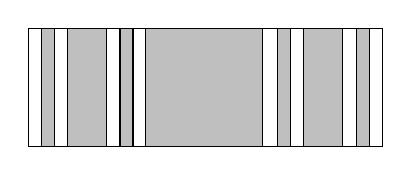
\begin{tikzpicture}[scale=0.5]
        \coordinate (A) at (0,0);
        \coordinate (B) at (9,0);
        \coordinate (C) at (9,-3);
        \coordinate (D) at (0,-3);       
        \coordinate (R) at ($(A)!0.33!(B)$);
        \coordinate (S) at ($(A)!0.66!(B)$);
        \coordinate (T) at ($(D)!0.33!(C)$);
        \coordinate (V) at ($(D)!0.66!(C)$);
        
        \draw (A) -- (B) -- (C) -- (D) -- cycle;
        \draw[fill=lightgray] (R) -- (S) -- (V) -- (T) -- cycle;
        
        \coordinate (A) at (0,0);
        \coordinate (B) at (3,0);
        \coordinate (C) at (3,-3);
        \coordinate (D) at (0,-3);       
        \coordinate (R) at ($(A)!0.33!(B)$);
        \coordinate (S) at ($(A)!0.66!(B)$);
        \coordinate (T) at ($(D)!0.33!(C)$);
        \coordinate (V) at ($(D)!0.66!(C)$);
        
        \draw[fill=lightgray] (R) -- (S) -- (V) -- (T) -- cycle;
        
        \coordinate (A) at (6,0);
        \coordinate (B) at (9,0);
        \coordinate (C) at (9,-3);
        \coordinate (D) at (6,-3);       
        \coordinate (R) at ($(A)!0.33!(B)$);
        \coordinate (S) at ($(A)!0.66!(B)$);
        \coordinate (T) at ($(D)!0.33!(C)$);
        \coordinate (V) at ($(D)!0.66!(C)$);
        
        \draw[fill=lightgray] (R) -- (S) -- (V) -- (T) -- cycle;
        
        \coordinate (A) at (0,0);
        \coordinate (B) at (1,0);
        \coordinate (C) at (1,-3);
        \coordinate (D) at (0,-3);       
        \coordinate (R) at ($(A)!0.33!(B)$);
        \coordinate (S) at ($(A)!0.66!(B)$);
        \coordinate (T) at ($(D)!0.33!(C)$);
        \coordinate (V) at ($(D)!0.66!(C)$);
        
        \draw[fill=lightgray] (R) -- (S) -- (V) -- (T) -- cycle;
        \coordinate (A) at (2,0);
        \coordinate (B) at (3,0);
        \coordinate (C) at (3,-3);
        \coordinate (D) at (2,-3);       
        \coordinate (R) at ($(A)!0.33!(B)$);
        \coordinate (S) at ($(A)!0.66!(B)$);
        \coordinate (T) at ($(D)!0.33!(C)$);
        \coordinate (V) at ($(D)!0.66!(C)$);
        
        \draw[fill=lightgray] (R) -- (S) -- (V) -- (T) -- cycle;
        \draw[fill=lightgray] (R) -- (S) -- (V) -- (T) -- cycle;
        \coordinate (A) at (6,0);
        \coordinate (B) at (7,0);
        \coordinate (C) at (7,-3);
        \coordinate (D) at (6,-3);       
        \coordinate (R) at ($(A)!0.33!(B)$);
        \coordinate (S) at ($(A)!0.66!(B)$);
        \coordinate (T) at ($(D)!0.33!(C)$);
        \coordinate (V) at ($(D)!0.66!(C)$);
        
        \draw[fill=lightgray] (R) -- (S) -- (V) -- (T) -- cycle;
        \draw[fill=lightgray] (R) -- (S) -- (V) -- (T) -- cycle;
        \coordinate (A) at (8,0);
        \coordinate (B) at (9,0);
        \coordinate (C) at (9,-3);
        \coordinate (D) at (8,-3);       
        \coordinate (R) at ($(A)!0.33!(B)$);
        \coordinate (S) at ($(A)!0.66!(B)$);
        \coordinate (T) at ($(D)!0.33!(C)$);
        \coordinate (V) at ($(D)!0.66!(C)$);
        
        \draw[fill=lightgray] (R) -- (S) -- (V) -- (T) -- cycle;
        \end{tikzpicture} 
        
    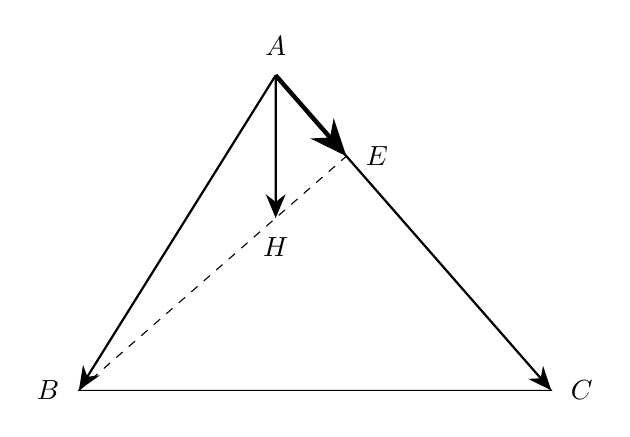
\begin{tikzpicture}
        \coordinate (A) at (2.5,4);
        \coordinate (B) at (0,0);
        \coordinate (C) at (6,0);
        \coordinate (E) at ($(A)!(B)!(C)$);
        \coordinate (D) at ($(B)!(A)!(C)$);
        \coordinate (H) at (intersection of A--D and B--E);
        
        \draw (A) -- (B) -- (C) -- cycle;
        \draw [dashed] (B) -- (E) ;
        \draw [thick,-{Stealth[scale=1.3,angle'=45]}] (A) -- (H) ;
        \draw [thick,-{Stealth[scale=1.3,angle'=45]}] (A) -- (B) ;
        \draw [thick,-{Stealth[scale=1.3,angle'=45]}] (A) -- (C) ;
        \draw [ultra thick,-{Stealth[scale=1.3,angle'=45]}] (A) -- (E) ;
        
        
         \foreach \v/\u/\t in 
         {A/90/$A$,
             B/180/$B$,
             C/0/$C$,
             H/270/$H$,
             E/0/$E$
            }
            {
                %\draw[ultra thick,fill] (\v) circle (2.5pt);
                \node[label=\u:\t] at (\v){};
            };     
    \end{tikzpicture}
    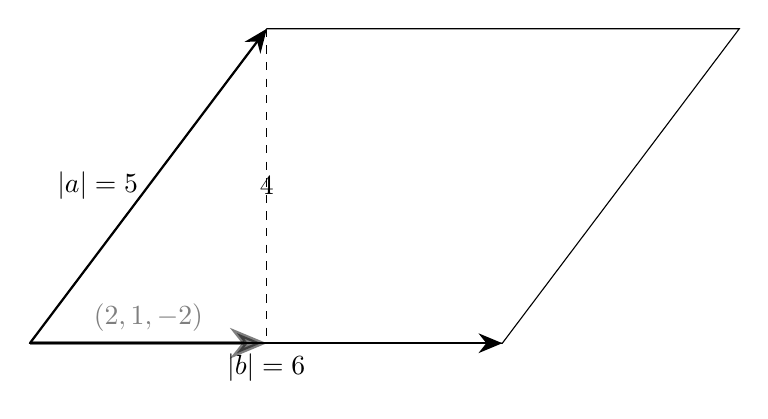
\begin{tikzpicture}
        \coordinate (O) at (0:0);
        \coordinate (A) at (53:5);
        \coordinate (mA) at (233:5);
        \coordinate (B) at (0:6);
        \coordinate (H) at ($(O)!(A)!(B)$);
        \draw (O) -- (A) -- ++(B) -- ++ (mA) -- cycle;
        \draw[dashed] (A) -- (H) node [midway, ]{$4$};
        
        \draw [thick,-{Stealth[scale=1.3,angle'=45]}] (O) -> (A) node [midway,left] {$|\lvec{a}|=5$};
        \draw [thick,-{Stealth[scale=1.3,angle'=45]}] (O) -> (B) node [midway,below] {$|\lvec{b}|=6$};
        \draw [color=black,ultra thick,-{Stealth[scale=1.3,angle'=45] } , opacity=0.5] (O) -> (H) node [midway,above] {$(2,1,-2)$};
    \end{tikzpicture}
    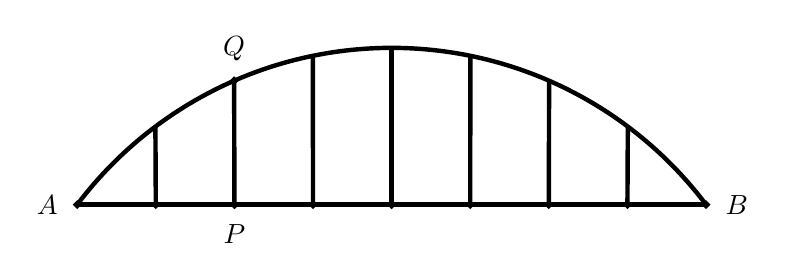
\begin{tikzpicture}[scale = 0.2]
                    
        \coordinate (A) at (143:25);
        \coordinate (B) at (37:25);
        
        \coordinate (P) at ($(A) !.25! (B) $);
        \coordinate (Q) at (5*2 -20, {sqrt((5*2-20) * ( 20-5*2)+625)});
        
        \foreach \v in {1,2,3,4,5,6,7}
        {
            \draw[ultra thick,fill] ($(A) !{0.125*\v}! (B)$) circle (2.5pt);
            \coordinate (T) at ($(A) !{0.125*\v}! (B)$);
            \coordinate (H) at (5*\v -20, {sqrt((5*\v-20) * ( 20-5*\v)+625)});
            \draw[ultra thick] (T) -- (H);
        };        
        
        
        \draw [ultra thick] (B) arc [radius=25, start angle=37, end angle= 143];
        \draw [ultra thick] (A) -- (B);
        \foreach \v/\u/\t in 
        {A/180/$A$,
         B/0/$B$,
         P/270/$P$,
         Q/90/$Q$
        }
        {
            \draw[ultra thick,fill] (\v) circle (2.5pt);
            \node[label=\u:\t] at (\v){};
        };     
    \end{tikzpicture}
            
    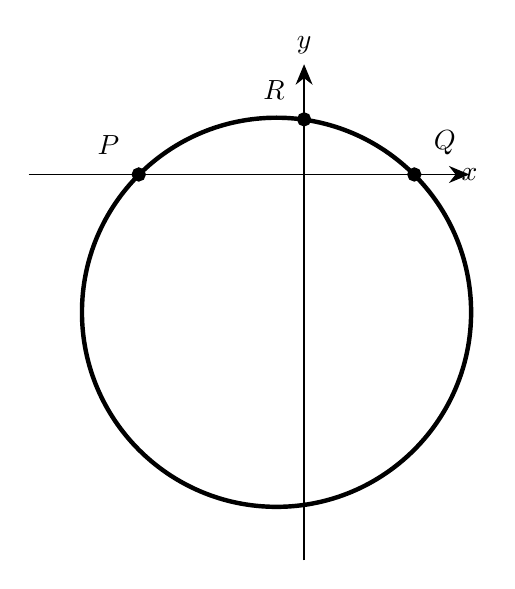
\begin{tikzpicture}[scale=0.7]
        \draw[ultra thick] (-0.5,-2.5) circle (3.53);
        \coordinate (P) at (-3,0);
        \coordinate (Q) at (2,0);
        \coordinate (R) at (0,1);
        
        \foreach \v/\u/\t in 
        {P/135/$P$,
         Q/45/$Q$,
         R/135/$R$
        }
        {
            \draw[ultra thick,fill] (\v) circle (2.5pt);
            \node[label=\u:\t] at (\v){};
        };        
        \draw[-{Stealth[scale=1.3,angle'=45]},semithick] (-5,0) -- (3,0) node[] {$x$};
        \draw[-{Stealth[scale=1.3,angle'=45]},semithick] (0,-7) -- (0,2)   node[above] {$y$};
                
        
    \end{tikzpicture}
   	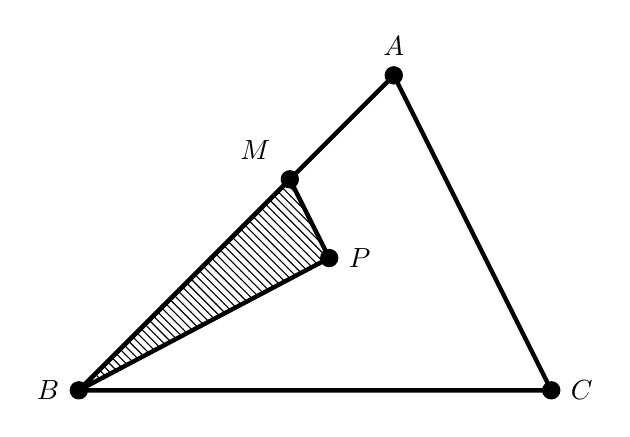
\begin{tikzpicture}
    \newcommand{\BX}{-4};
    \newcommand{\BY}{-4};
    \newcommand{\CX}{2};
    \newcommand{\CY}{-4};
    \coordinate (cAPt) at (0,0);
    \coordinate (cBPt) at (\BX, \BY);
    \coordinate (cCPt) at (\CX, \CY);
    \coordinate (cPPt) at ({\BX*0.33 + \CX*0.25}, {\BY*0.33+\CY * 0.25});
    \coordinate (cMPt) at ($(cAPt) !.33! (cBPt) $);
    \draw [ ultra thick] (cAPt) --(cBPt) -- (cCPt) -- (cAPt) circle;
    \draw [ pattern=north west lines, ultra thick] (cBPt) --(cMPt) -- (cPPt) -- (cBPt) ;
    \foreach \v/\u/\t in 
    {cAPt/90/$A$,
        cBPt/180/$B$,
        cCPt/0/$C$,
        cPPt/0/$P$,
        cMPt/135/$M$
    }
    {
        \draw[ultra thick,fill] (\v) circle (2.5pt);
        \node[label=\u:\t] at (\v){};
    };
    \end{tikzpicture}
    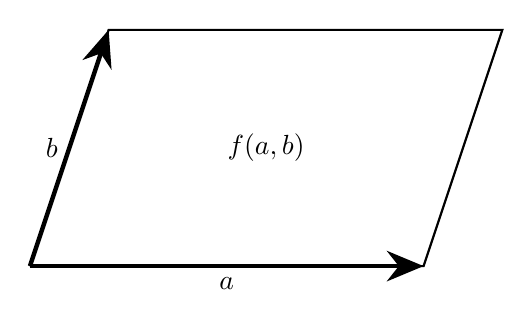
\begin{tikzpicture}
    
    \draw [thick] (0,0) -- ++(1,3) -- ++(5,0) -- ++(-1,-3) -- ++(-5,0) ;
    \draw [ultra thick, -{Stealth[scale=1.3,angle'=45]}] (0,0) -- (5,0) node [midway,below]{$\lvec{a}$};
    \draw [ultra thick, -{Stealth[scale=1.3,angle'=45]}] (0,0) -- (1,3) node [midway, left] {$\lvec{b}$};
    \node at (3,1.5){$f(\lvec{a}, \lvec{b})$};
    \end{tikzpicture}
    \begin{tikzpicture}
        %限定輸出區塊
        
        \clip (-3.5,-5.5) rectangle (3.5, 5.5); 
        
        \draw[-{Stealth[scale=1.3,angle'=45]},semithick] (-3,0) -- (3,0) node[] {$x$};
        \draw[-{Stealth[scale=1.3,angle'=45]},semithick] (0,-5) -- (0,5)   node[above] {$y$};
        
        \draw[thick, color=black, domain=-3:3, name path=L1] plot (\x,{0.5*\x+2}) ;
        \draw[thick, color=black, domain=-3:3, name path=L2] plot (\x,{2*\x-2});
        \draw[thick, color=black, domain=-3:3, , name path=L3] plot (\x,{-2*\x-4});
        \path [name intersections={of = L1 and L2}];
        \coordinate (A)  at (intersection-1);
        \path [name intersections={of = L1 and L3}];
        \coordinate (B)  at (intersection-1);
        \path [name intersections={of = L2 and L3}];
        \coordinate (C)  at (intersection-1);
        
        \foreach \v in 
        {A,B,C}
        {
            \draw[ultra thick,fill] (\v) circle (2pt);
        };        
        \node [above left] at (A) {$A$};
        \node [left] at (B) {$B$};
        \node [left] at (C) {$C$};

    \end{tikzpicture}
    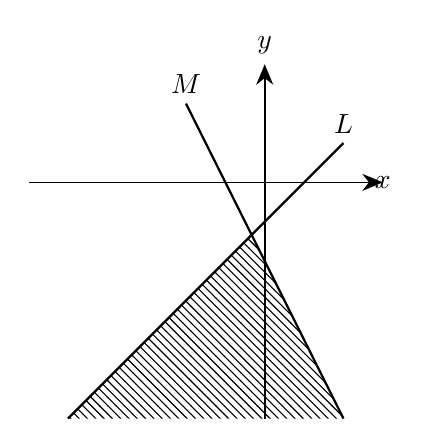
\begin{tikzpicture}[scale=0.5]
    \coordinate (A) at (2, 1);
    \coordinate (B) at (-2, -3);
    \coordinate (C) at (-2, 2);
    \coordinate (D) at (2, -6);
    \coordinate (E) at (-0.33, -1.33);
    \coordinate (F) at (-5, -6);
    
    \draw[-{Stealth[scale=1.3,angle'=45]},semithick] (-6,0) -- (3,0) node[] {$x$};
    \draw[-{Stealth[scale=1.3,angle'=45]},semithick] (0,-6) -- (0,3)   node[above] {$y$};
    
    \draw [thick] (A) -- (F) ;
    \draw [thick] (C) -- (D) ;
    
    \fill [pattern=north west lines] (D) -- (E)--(F)--(D)  circle ;
    
    \node [above] at (A) {$L$};
    \node [above] at (C) {$M$};
    
    \end{tikzpicture}
    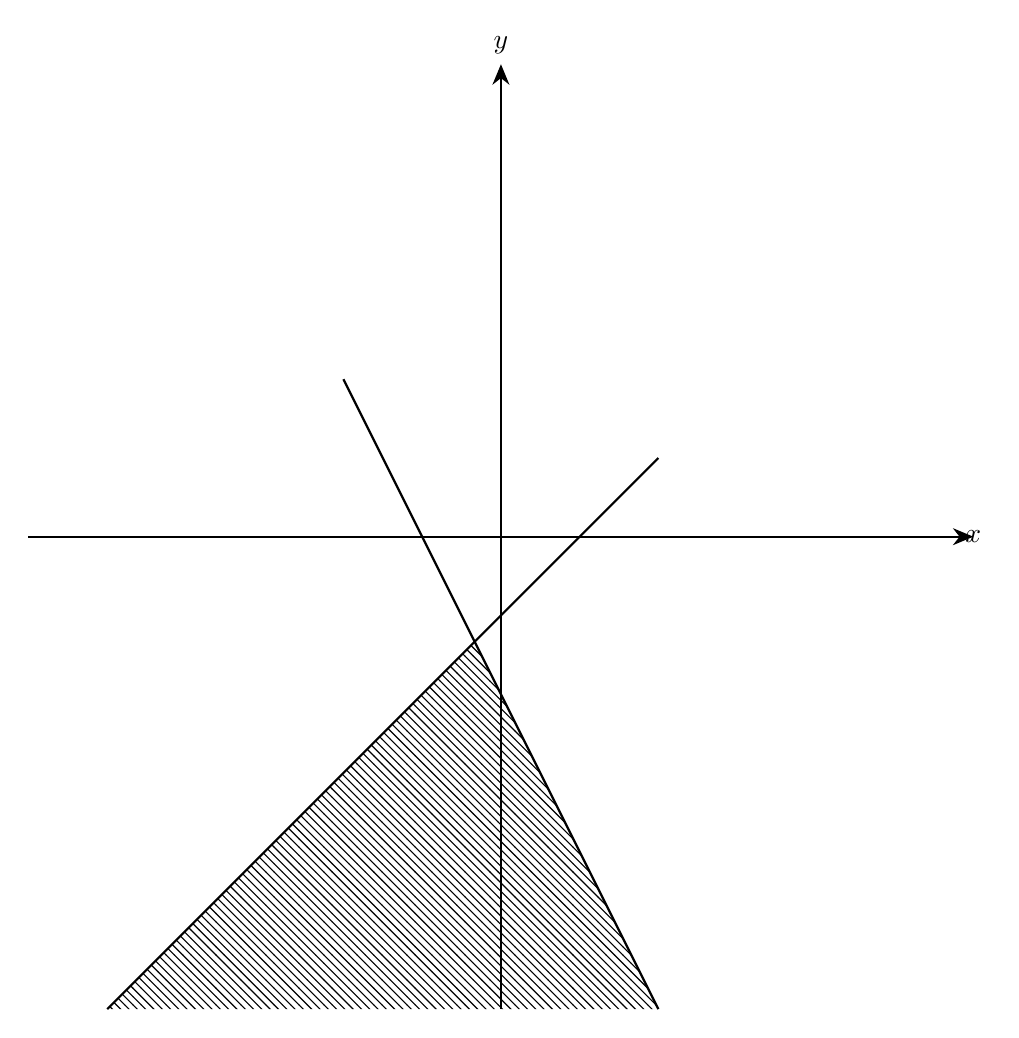
\begin{tikzpicture}
        \coordinate (A) at (2, 1);
        \coordinate (B) at (-2, -3);
        \coordinate (C) at (-2, 2);
        \coordinate (D) at (2, -6);
        \coordinate (E) at (-0.33, -1.33);
        \coordinate (F) at (-5, -6);
        
        
        \draw[-{Stealth[scale=1.3,angle'=45]},semithick] (-6,0) -- (6,0) node[] {$x$};
        \draw[-{Stealth[scale=1.3,angle'=45]},semithick] (0,-6) -- (0,6)   node[above] {$y$};
        \draw [ thick] (A) -- (F) ;
        \draw [thick] (C) -- (D) ;
        \fill [pattern=north west lines] (D) -- (E)--(F)--(D)  circle ;
        
    \end{tikzpicture}
    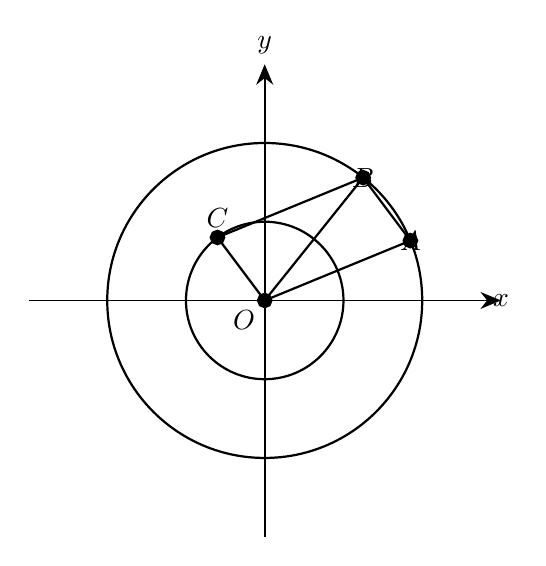
\begin{tikzpicture}
        \coordinate (O) at (0,0);
        \coordinate (A) at (1.85, 0.76);
        \coordinate (B) at (1.25, 1.56);
        \coordinate (C) at (-0.6, 0.8);
        
        
        \draw[thick] (O) circle (2);
        \draw[thick] (O) circle (1);
        
        \draw [ thick] (O)--(A) --(B) --(C) --(O) circle;
        \draw[thick] (O) --(B);
        
        \foreach \v in 
        {O,A,B,C}
        {
            \draw[ultra thick,fill] (\v) circle (2pt);
        };        
        % x軸 y 軸 axes
        \draw[-{Stealth[scale=1.3,angle'=45]},semithick] (-3,0) -- (3,0) node[] {$x$};
        \draw[-{Stealth[scale=1.3,angle'=45]},semithick] (0,-3) -- (0,3)   node[above] {$y$};
        \node[] at (A){$A$};
        \node[] at (B){$B$};
        \node[below left] at (O){$O$};
        \node[above] at (C){ $C$};
    \end{tikzpicture}
    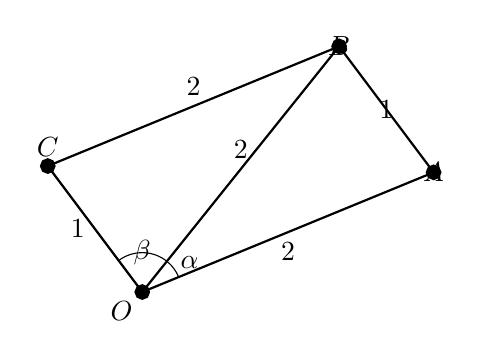
\begin{tikzpicture}[scale=2]
    \coordinate (O) at (0,0);
    \coordinate (A) at (1.85, 0.76);
    \coordinate (B) at (1.25, 1.56);
    \coordinate (C) at (-0.6, 0.8);

    
    \draw [ thick] (O)--(A) node [midway, below ]{2};
    \draw [ thick] (O)--(B) node [midway, above ]{2};
    \draw [ thick] (B)--(C) node [midway, above]{2};
    \draw [ thick] (O)--(C) node [midway, left]{1};
    \draw [ thick] (A)--(B) node [midway,]{1};
   
    \foreach \v in 
    {O,A,B,C}
    {
        \draw[ultra thick,fill] (\v) circle (1pt);
    };        
    %標示 \ahpha \beta 角
	\pic [draw, -, "", angle eccentricity=2.5] {angle = A--O--B};
    \node[label={[shift={(0.6,0.05)}]$\alpha$}] at (O) {};	
	\pic [draw, -, "", angle eccentricity=2.5] {angle = B--O--C};
    \node[label={[shift={(0,0.1)}]$\beta$}] at (O) {};	
    
    \node[] at (A){$A$};
    \node[] at (B){$B$};
    \node[below left] at (O){$O$};
    \node[above] at (C){ $C$};
    \end{tikzpicture}

        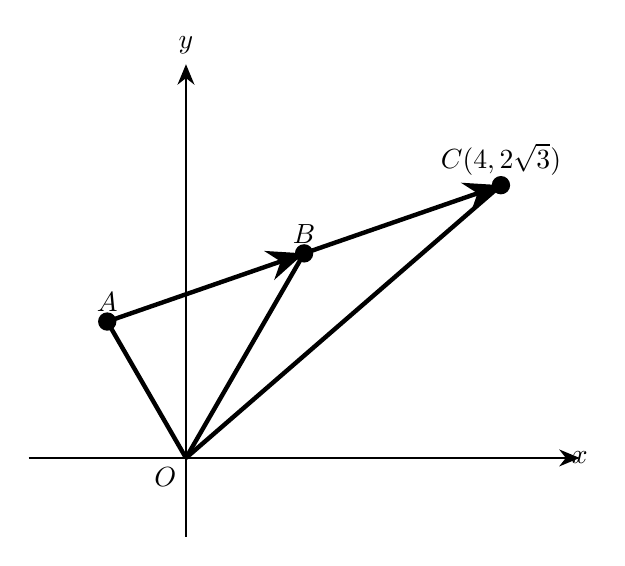
\begin{tikzpicture}
            \coordinate (A) at (120:2);
            \coordinate (B) at (60:3);
            \coordinate (C) at  ($ (A) !2! (B) $); 
            \coordinate (O) at (0,0);
            \draw [ultra thick,-{Stealth[scale=1.3,angle'=45]}] (A) -- (B) ;        
            \draw [ultra thick,-{Stealth[scale=1.3,angle'=45]}] (B) -- (C) ;
            \draw [ultra thick] (O) -- (A) ;
            \draw [ultra thick] (O) -- (B) ;
            \draw [ultra thick] (O) -- (C) ;
            
            
        \foreach \v/\u/\t in 
        {A/180/$A$,
         B/90/$B$,
         C/90/$C$
        }
        {
            \draw[ultra thick,fill] (\v) circle (2.5pt);
        };
        
        \node[above] at (A){$A$};
        \node[above] at (B){$B$};
        \node[below left] at (O){$O$};
        \node[above] at (C){ $C(4, 2 \sqrt{3})$ };
        
        
        
        % x軸 y 軸 axes
        \draw[-{Stealth[scale=1.3,angle'=45]},semithick] (-2,0) -- (5,0) node[] {$x$};
        \draw[-{Stealth[scale=1.3,angle'=45]},semithick] (0,-1) -- (0,5)   node[above] {$y$};
        \end{tikzpicture}
        
        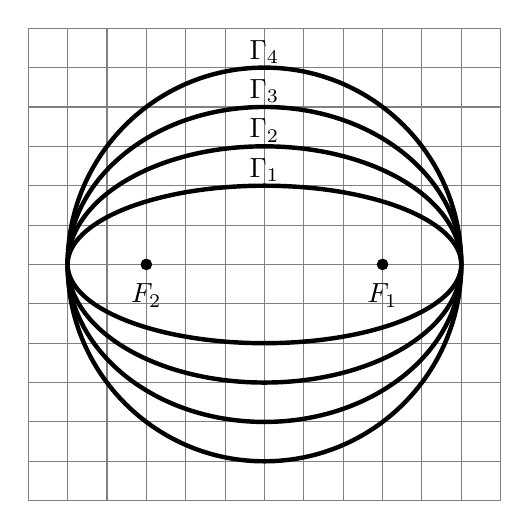
\begin{tikzpicture}[scale=0.5]
        \draw[color=gray, step=1] (-6,-6) grid (6,6);
        \draw [ultra thick](0,0) ellipse (5 and 2);
        \draw [ultra thick](0,0) ellipse (5 and 3);
        \draw [ultra thick](0,0) ellipse (5 and 4);
        \draw [ultra thick](0,0) ellipse (5 and 5);

        
        \coordinate (cF1Pt) at (3, 0);
        \coordinate (cF2Pt) at (-3, 0);
        
        \foreach \v/\u/\t in 
        {cF1Pt/270/$F_1$,
            cF2Pt/270/$F_2$
        }
        {
            \draw[ultra thick,fill] (\v) circle (2.5pt);
            \node[label=\u:\t] at (\v){};
        };
        
        \node at (0,2.4) {$\Gamma_1$};
        \node at (0,3.4) {$\Gamma_2$};
        \node at (0,4.4) {$\Gamma_3$};
        \node at (0,5.4) {$\Gamma_4$};
        
        \end{tikzpicture}
    \begin{tikzpicture}[scale=0.5]
        \draw[color=gray, step=1] (-4,-10) grid (6,10);
        \draw[thick, color=black, domain=0:6] plot (\x,{sqrt(12*\x)});
        \draw[thick, color=black, domain=0:6] plot (\x,{-sqrt(12*\x)});
        \coordinate (cAPt) at (0.2, {sqrt(12 * 0.2)});
        \coordinate (cBPt) at (0.8, {sqrt(12 * 0.8)});
        \coordinate (cCPt) at (1.2, {sqrt(12 * 1.2)});
        \coordinate (cDPt) at (1.8, {sqrt(12 * 1.8)});
        \coordinate (cEPt) at (2.8, {sqrt(12 * 2.8)});
        \draw [ultra thick, dashed](-4,0) -- (6,0) ;
        \node [] at (6,0) {軸};
        
       \foreach \v/\u/\t in 
       {cAPt/180/$A$,
        cBPt/180/$B$,
        cCPt/180/$C$,
        cDPt/180/$D$,
        cEPt/180/$E$
        }
        {
            \draw[ultra thick,fill] (\v) circle (2.5pt);
            \node[label=\u:\t] at (\v){};
        };
    \end{tikzpicture}
    
        \begin{tikzpicture}[scale=0.5]
        \draw[color=gray, step=1] (-4,-10) grid (6,10);
        \draw[thick, color=black, domain=0:6] plot (\x,{sqrt(12*\x)});
        \draw[thick, color=black, domain=0:6] plot (\x,{-sqrt(12*\x)});
        \coordinate (cAPt) at (0.2, {sqrt(12 * 0.2)});
        \coordinate (cBPt) at (0.8, {sqrt(12 * 0.8)});
        \coordinate (cCPt) at (1.2, {sqrt(12 * 1.2)});
        \coordinate (cDPt) at (1.8, {sqrt(12 * 1.8)});
        \coordinate (cEPt) at (2.8, {sqrt(12 * 2.8)});
        \coordinate (cFPt) at (3, 0);
        
        \draw [ultra thick, dashed](-4,0) -- (6,0) ;
        \node [] at (6,0) {軸};
        \draw [ultra thick, dashed](-3,-10) -- (-3,10) ;
        \node [above] at (-3,10) {準線$L$};
        \foreach \v/\u/\t in 
        {cAPt/180/$A$,
            cBPt/180/$B$,
            cCPt/180/$C$,
            cDPt/180/$D$,
            cEPt/180/$E$,
            cFPt/45/$F$
        }
        {
            \draw[ultra thick,fill] (\v) circle (2.5pt);
            \node[label=\u:\t] at (\v){};
        };
        \end{tikzpicture}
    
        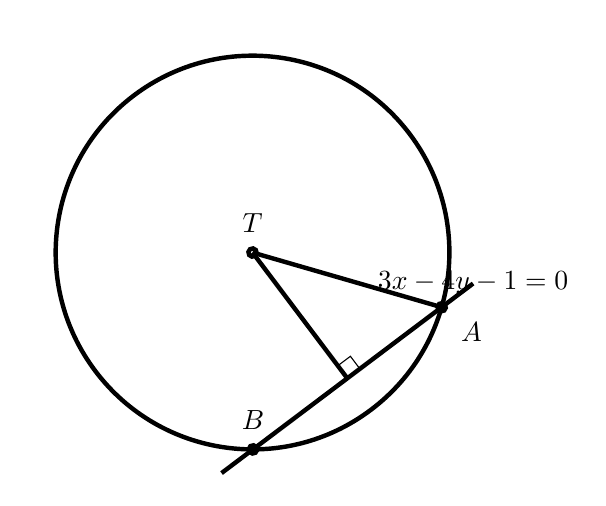
\begin{tikzpicture}[scale=0.5]
        \begin{scope}[rotate=37] 
        
        \coordinate (cOPt) at (0:0);
        \coordinate (cAPt) at (3,-4);
        \coordinate (cBPt) at (-3,-4);
        \coordinate (cAPtExtend) at (4,-4);
        \coordinate (cBPtExtend) at (-4,-4);
        \coordinate (cHPt) at ($(cAPt)!(cOPt)!(cBPt)$);

        \draw [ultra thick](cAPtExtend) --(cBPtExtend) ;
        \draw [ultra thick] (cHPt)--(cOPt) ; 
        \draw [ultra thick] (cAPt)--(cOPt) ; 
        
%        \draw [ultra thick](cOPt) --(cRPt) ;
            \newcommand{\nRect}{0.4cm}
            \def\rectanglepath{-- +(+\nRect,0cm) -- +(+\nRect,+\nRect) -- +(0cm,\nRect) -- cycle} 
            \draw (cHPt) \rectanglepath;
        \draw[ultra thick] (cAPt) circle (3pt);
        \draw[ultra thick] (cBPt) circle (3pt);
        \draw[ultra thick] (cOPt) circle (3pt);
        
        \draw[ultra thick] (cOPt) circle (5);
        
        \node[label=90:$T$] at (cOPt){};

        \node[label=90:$B$] at (cBPt){};
        \node[label=330:$A$] at (cAPt){};
        \node[] at (cAPtExtend){$3x-4y-1=0$};
        \end{scope}
        
        
        \end{tikzpicture}
        
       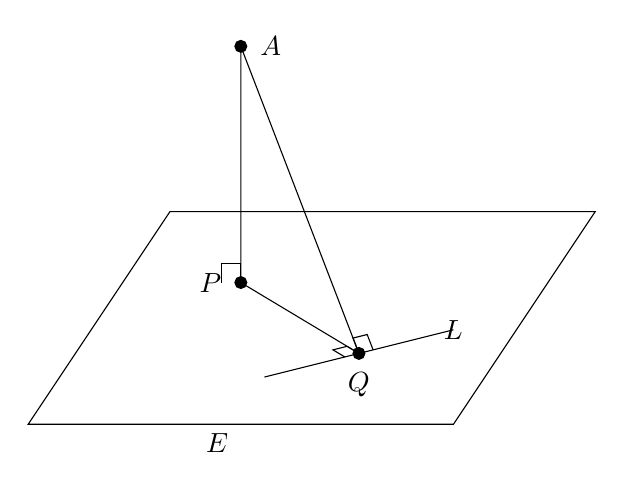
\begin{tikzpicture}[scale=0.6]
       %設定立體空間的平面方程式中在坐標平面上的2個向量
       \pgfmathsetmacro{\EAlphaVectorX}{9}
       \pgfmathsetmacro{\EAlphaVectorY}{0}
       \pgfmathsetmacro{\EBetaVectorX}{3}
       \pgfmathsetmacro{\EBetaVectorY}{4.5}
       
       \coordinate (cPPt) at (4.5,3);
       
       \coordinate (cQPt) at (7,1.5);
       \coordinate (cVectorPP) at (4,4);
       \coordinate (cNVector) at (0,5); 
       
       \coordinate (cLVector) at (2,0.5);
       \coordinate (cMLVector) at (-2,-0.5);
       \coordinate (cLStartPt) at ($(cQPt) + (cLVector)$);
       
       \coordinate (cAPt) at ($(cPPt) + (cNVector)$);
       \coordinate (cNVectorEndPt) at ($(cPPt) + (cNVector)$);
       
       \coordinate (cminQAVector) at ($0.05*(cAPt) - 0.05*(cQPt)$);
       \coordinate (cmQAVector) at ($-0.05*(cAPt) + 0.05*(cQPt)$);
       \coordinate (cmLVector) at ($0.15*(cLVector)$);
       \coordinate (cmmLVector) at ($-0.15*(cLVector)$);
       
       \coordinate (cmQPVector) at ($0.1*(cPPt) - 0.1*(cQPt)$);
        \coordinate (cmmQPVector) at ($-1*(cmQPVector)$);
        
        %畫出平面方程式
       \draw (0,0) -- ++(\EAlphaVectorX, \EAlphaVectorY) -- ++(\EBetaVectorX, \EBetaVectorY) -- ++(-\EAlphaVectorX, -\EAlphaVectorY) -- ++(-\EBetaVectorX, -\EBetaVectorY) -- cycle;
       
       \draw (cPPt) -- (cAPt);
       \draw (cPPt) -- (cQPt);
       \draw (cAPt) -- (cQPt);
       \draw (cQPt) -- ++(cLVector);
       \draw (cQPt) -- ++(cMLVector);
        
        %劃出垂直記號
        \newcommand{\nRect}{0.4};
        \draw (cPPt) -- ++(0,\nRect) -- ++(-\nRect,0) -- ++(0,-\nRect) ; 
        \draw (cQPt) -- ++(cminQAVector) -- ++(cmLVector) -- ++( cmQAVector);
        \draw (cQPt) -- ++(cmQPVector) -- ++(cmmLVector) -- ++ (cmmQPVector);
        
       \foreach \v/\u/\t in 
       {cPPt/180/$P$,
           cQPt/270/$Q$,
           cNVectorEndPt/0/$A$
        }
        {
            \draw[ultra thick,fill] (\v) circle (2.5pt);
            \node[label=\u:\t] at (\v){};
        };
        \node[below] at (4,0){$E$};
        \node[] at (cLStartPt) {$L$};
        %       
        \end{tikzpicture}
        
        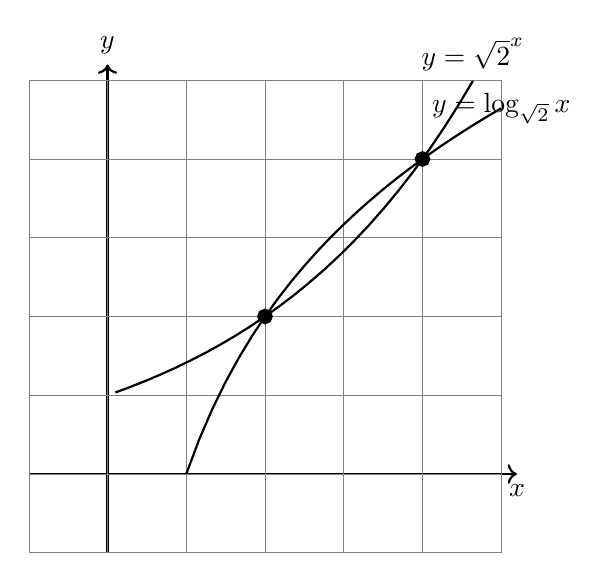
\begin{tikzpicture}
        \draw[thick, ->] (-1,0) -- (5.2,0) node[below] {$x$};
        \draw[thick, ->] (0,-1) -- (0,5.2) node[above] {$y$};
        \draw[very thin,color=gray] (-1,-1) grid (5,5);
        \draw[thick, color=black, domain=0.1:4.64] plot (\x,{2^(\x/2)});
        \draw[thick, color=black, domain=1:5] plot (\x, {log10(\x)/log10(sqrt(2))});
        \node[above] at (4.64, 5) {$y=\sqrt{2}^x$};
        \node[] at (5,4.64 ) {$y=\log_{\sqrt{2}} x$};
        \draw[ultra thick,fill] (2,2) circle (2pt);
        \draw[ultra thick,fill] (4,4) circle (2pt);
        \end{tikzpicture}
        
        
    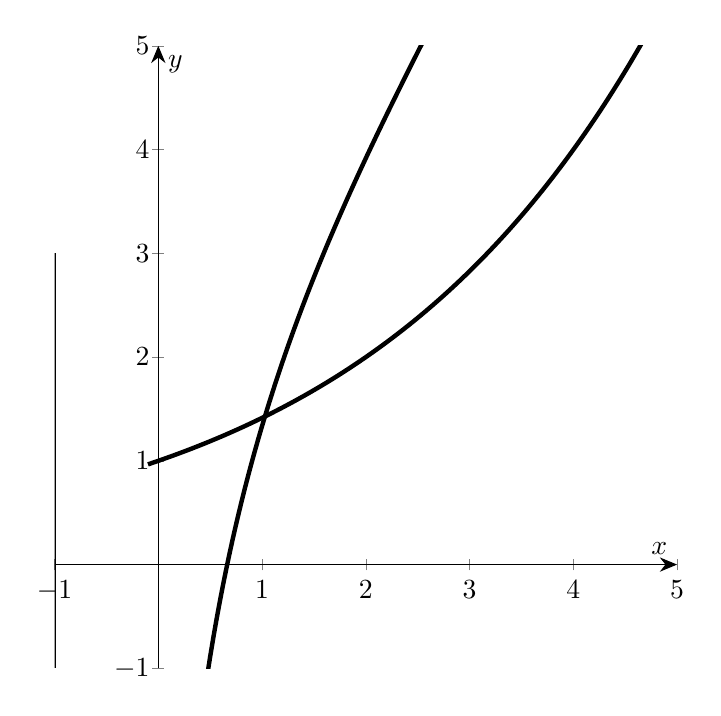
\begin{tikzpicture}[scale=1.0]
    \pgfmathdeclarefunction{polyAAA}{0}{%
        \pgfmathparse{ln(x)/ln(sqrt(2))}%
    }
    \pgfmathdeclarefunction{polyBBB}{0}{%
    \pgfmathparse{2^(x/2)}%
    }
    \begin{axis}[
    unit vector ratio*=1 1 1,
    axis lines = middle,
    axis line style =  {-{Stealth[scale=1.3,angle'=45]}},
    width=11cm,
    xlabel={$x$},
    ylabel={$y$},
    domain=-1:5,
    ymin=-1,
    ymax=+5,
    xmin=-1,
    xmax=+5,
    xtick={-1,0,1,2,3,4,5},
    ytick={-1,0,1,2,3,4,5},
    samples=160,
    stack plots=y,
    y tick label style={, xshift=0.25em}
    ]
    \draw[thick] (axis cs:-1,-1) -- (axis cs:-1,3);
    
    \addplot[black,ultra thick,mark=none,stack plots=y, domain=-0.1:5] {polyBBB};
    
    
    \addplot[black,ultra thick,mark=none,stack plots=y, domain=0.1:5] {polyAAA};
    

    \node at (axis cs:-1, -1.5) {$x=-1$};
    
    \end{axis}
    \end{tikzpicture}
    
            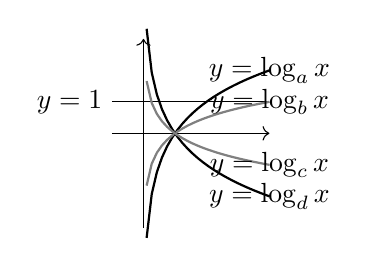
\begin{tikzpicture}[xscale=0.4,yscale=0.4]
            %\draw[->] (-3.2,0) -- (3.2,0) node[below] {$x$};
            %\draw[->] (0,-3.2) -- (0,3.2) node[above] {$f(x)$};
            
            %\draw (-5,-5) -- (5,-5) -- (5,5) -- (-5,5) -- cycle;
            \draw [->](-1,-0) -- (4,0);
            \draw [->](0,-3) -- (0,3);
            \draw (-1,1) -- (4,1);
            \draw[thick,color=black, domain=0.1:4] plot (\x, {log2( \x)});
            \draw[thick,color=gray, domain=0.1:4] plot (\x, {0.5*log2( \x)});
            \draw[thick,color=black, domain=0.1:4] plot (\x, {-log2( \x)});
            \draw[thick,color=gray, domain=0.1:4] plot (\x, {-0.5*log2( \x)});
            
            \node [] at (4,2) {$y=\log_a x$ };
            \node [] at (4,1) {$y=\log_b x$ };
            \node [] at (4,-1) {$y=\log_c x$ };
            \node [] at (4,-2) {$y=\log_d x$ };
            \node [left] at (-1,1) {$y=1$ };
            \end{tikzpicture}
            
        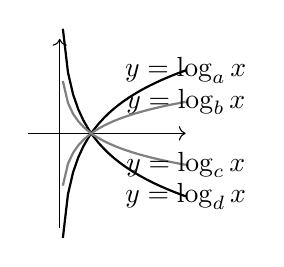
\begin{tikzpicture}[xscale=0.4,yscale=0.4]
        %\draw[->] (-3.2,0) -- (3.2,0) node[below] {$x$};
        %\draw[->] (0,-3.2) -- (0,3.2) node[above] {$f(x)$};
        
        %\draw (-5,-5) -- (5,-5) -- (5,5) -- (-5,5) -- cycle;
        \draw [->](-1,-0) -- (4,0);
        \draw [->](0,-3) -- (0,3);
        \draw[thick,color=black, domain=0.1:4] plot (\x, {log2( \x)});
        \draw[thick,color=gray, domain=0.1:4] plot (\x, {0.5*log2( \x)});
        \draw[thick,color=black, domain=0.1:4] plot (\x, {-log2( \x)});
        \draw[thick,color=gray, domain=0.1:4] plot (\x, {-0.5*log2( \x)});
        
        \node [] at (4,2) {$y=\log_a x$ };
        \node [] at (4,1) {$y=\log_b x$ };
        \node [] at (4,-1) {$y=\log_c x$ };
        \node [] at (4,-2) {$y=\log_d x$ };
        \end{tikzpicture}
        
        \begin{tikzpicture}[xscale=0.4,yscale=0.4]
        %\draw[->] (-3.2,0) -- (3.2,0) node[below] {$x$};
        %\draw[->] (0,-3.2) -- (0,3.2) node[above] {$f(x)$};
        
        %\draw (-5,-5) -- (5,-5) -- (5,5) -- (-5,5) -- cycle;
        \draw [->](-4,-0) -- (4,0);
        \draw [->](0,-3) -- (0,3);
        \draw[thick,color=black, domain=0.1:4] plot (\x, {log2( abs(\x))});
        \draw[thick,color=black, domain=-4:-0.1] plot (\x, {log2( abs(\x))});
        
        \draw[thick,color=gray, domain=-2:4] plot (\x, {\x -1});
        %畫出近似值交點
        \draw[thick,fill] (1,0) circle (2pt);
        \draw[thick,fill] (2,1) circle (2pt);
        \draw[thick,fill] (-0.38,-1.38) circle (2pt);
        \node [below] at (0,-3) {圖五};
        \end{tikzpicture}
        
        \begin{tikzpicture}[xscale=0.2,yscale=0.2]
        
        %\draw[->] (-3.2,0) -- (3.2,0) node[below] {$x$};
        %\draw[->] (0,-3.2) -- (0,3.2) node[above] {$f(x)$};
        
        %\draw (-5,-5) -- (5,-5) -- (5,5) -- (-5,5) -- cycle;
        \draw [->](-5,-0) -- (5,0);
        \draw [->](0,-1) -- (0,5.6);
        
        \draw[thick,color=gray, domain=-2.1:2.1] plot (\x, {4-\x *\x});
        \draw[thick,color=black, domain=0.03:4.5] plot (\x, {abs(log2(\x))});
        
        %畫出近似值交點
        \draw[ultra thick,fill] (1.78,0.83) circle (2pt);
        \draw[ultra thick,fill] (0.06,3.99) circle (2pt);
        \node [below] at (0,-1) {圖四};
        \end{tikzpicture}
            
        \begin{tikzpicture}[xscale=0.2,yscale=0.1]
        %\draw[->] (-3.2,0) -- (3.2,0) node[below] {$x$};
        %\draw[->] (0,-3.2) -- (0,3.2) node[above] {$f(x)$};
        
        %\draw (-5,-5) -- (5,-5) -- (5,5) -- (-5,5) -- cycle;
        \draw [->](-5,-0) -- (5,0);
        \draw [->](0,-1) -- (0,20);

        \draw[thick,color=gray, domain=-4.5:4.5] plot (\x, {\x *\x});
        \draw[thick,color=black, domain=-4.5:4.5] plot (\x, {2^( abs(\x))});
        %畫出近似值交點
        \draw[ultra thick,fill] (2,4) circle (4pt);
        \draw[ultra thick,fill] (4,16) circle (4pt);
        \draw[ultra thick,fill] (-2,4) circle (4pt);
        \draw[ultra thick,fill] (-4,16) circle (4pt);
        \node [below] at (0,-1) {圖三};
        \end{tikzpicture}

        \begin{tikzpicture}[scale=0.2]
        %\draw[->] (-3.2,0) -- (3.2,0) node[below] {$x$};
        %\draw[->] (0,-3.2) -- (0,3.2) node[above] {$f(x)$};
        
        %\draw (-5,-5) -- (5,-5) -- (5,5) -- (-5,5) -- cycle;
        \draw [->](-4,-0) -- (4,0);
        \draw [->](0,-1) -- (0,9);
        \draw[thick,color=black, domain=0.5:4] plot (\x, {log2( abs(\x))});
        \draw[thick,color=black, domain=-4:-0.5] plot (\x, {log2( abs(\x))});
        \draw[thick,color=gray, domain=-4:4] plot (\x, {0.5^( abs(\x))});
        %畫出近似值交點
        \draw[ultra thick,fill] (1.32,0.4) circle (6pt);
        \draw[ultra thick,fill] (-1.32,0.4) circle (6pt);
        \node [below] at (0,-1) {圖二};
        \end{tikzpicture}
        
        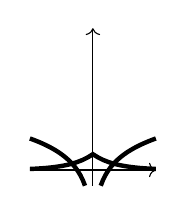
\begin{tikzpicture}[scale=0.2]
        %\draw[->] (-3.2,0) -- (3.2,0) node[below] {$x$};
        %\draw[->] (0,-3.2) -- (0,3.2) node[above] {$f(x)$};
        
        %\draw (-5,-5) -- (5,-5) -- (5,5) -- (-5,5) -- cycle;
        \draw [->](-4,-0) -- (4,0);
        \draw [->](0,-1) -- (0,9);
        \draw[ultra thick,color=black, domain=0.5:4] plot (\x, {log2( abs(\x))});
        \draw[ultra thick,color=black, domain=-4:-0.5] plot (\x, {log2( abs(\x))});
        \draw[ultra thick,color=black, domain=-4:4] plot (\x, {0.5^( abs(\x))});
        %\draw[ultra thick,fill] (0,2) circle (6pt);
        
        \end{tikzpicture}
        
        \begin{tikzpicture}[scale=0.2]
        %\draw[->] (-3.2,0) -- (3.2,0) node[below] {$x$};
        %\draw[->] (0,-3.2) -- (0,3.2) node[above] {$f(x)$};
        
        %\draw (-5,-5) -- (5,-5) -- (5,5) -- (-5,5) -- cycle;
        \draw [->](-4,-0) -- (4,0) ;
        \draw [->](0,-1) -- (0,9) ;
        \draw[thick,color=black, domain=-1.5:1.5] plot (\x, {4^(\x) + 0.25^(\x)});
        \draw[thick] (-4,2) -- (4,2) ;
        
        \draw[ultra thick,fill] (0,2) circle (6pt);
        \node [below] at (0,-1) {圖一};
        \end{tikzpicture}
        
        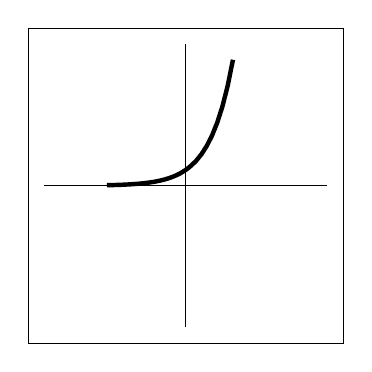
\begin{tikzpicture}[scale=0.2]
        %\draw[->] (-3.2,0) -- (3.2,0) node[below] {$x$};
        %\draw[->] (0,-3.2) -- (0,3.2) node[above] {$f(x)$};
        \draw (-10,-10) -- (10,-10) -- (10,10) -- (-10,10) -- cycle;
        \draw (-9,-0) -- (9,0) ;
        \draw (0,-9) -- (0,9) ;
        %\draw[very thin,color=gray] (-3,-3) grid (3,3);
        %\draw[color=orange, domain=-3:3] plot (\x,\x);
        %\draw[color=blue, domain=-3:3] plot (\x,{sin(\x r)});
        %\draw[color=red, domain=-3:3] plot (\x,{\x-(1/6)*(\x)^3});
        \draw[ultra thick,color=black, domain=-5:3] plot (\x, {2^(\x)});
        \end{tikzpicture}
        
    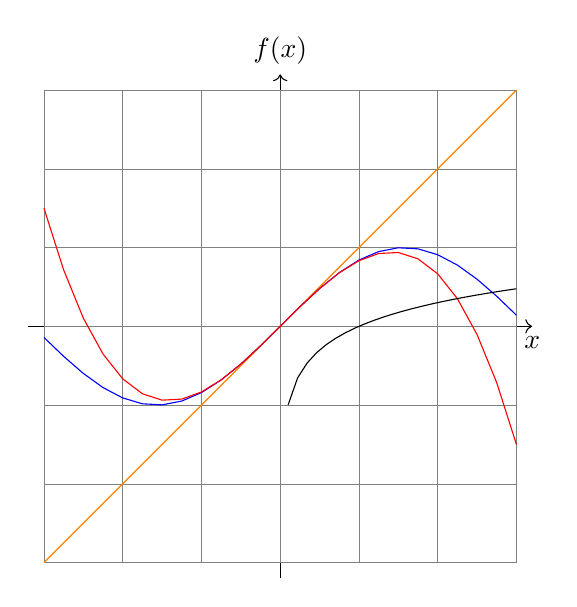
\begin{tikzpicture}
    \draw[->] (-3.2,0) -- (3.2,0) node[below] {$x$};
    \draw[->] (0,-3.2) -- (0,3.2) node[above] {$f(x)$};
    \draw[very thin,color=gray] (-3,-3) grid (3,3);
    \draw[color=orange, domain=-3:3] plot (\x,\x);
    \draw[color=blue, domain=-3:3] plot (\x,{sin(\x r)});
    \draw[color=red, domain=-3:3] plot (\x,{\x-(1/6)*(\x)^3});
    \draw[color=black, domain=0.1:3.0] plot (\x, {log10(\x)});
    \end{tikzpicture}
    
    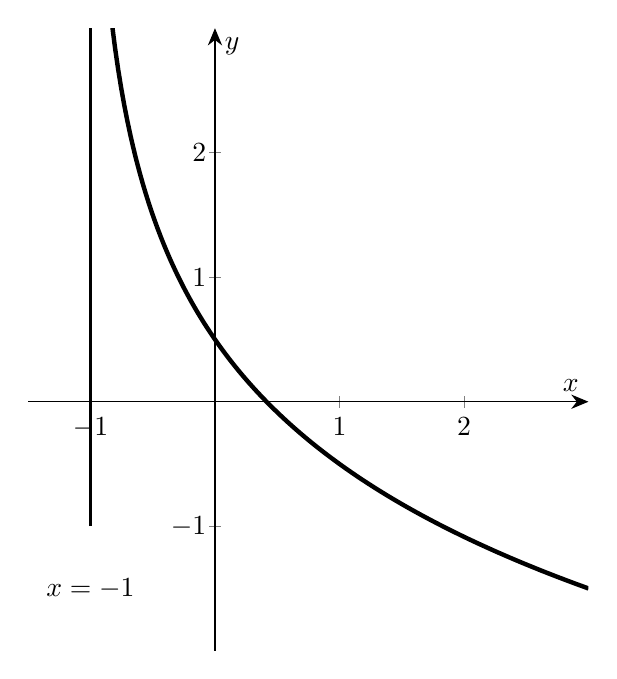
\begin{tikzpicture}[scale=1.0]
    \pgfmathdeclarefunction{polyAAA}{0}{%
        \pgfmathparse{ln(x+1)/ln(0.5)+0.5}%
    }
    \begin{axis}[
    unit vector ratio*=1 1 1,
    axis lines = middle,
    axis line style =  {-{Stealth[scale=1.3,angle'=45]}},
    width=11cm,
    xlabel={$x$},
    ylabel={$y$},
    domain=-2:14,
    ymin=-2,
    ymax=+3,
    xmin=-1.5,
    xmax=+3,
    xtick={-1,0,1,2},
    ytick={-1,0,1,2},
    samples=160,
    stack plots=y,
    y tick label style={, xshift=0.25em}
    ]
    \draw[thick] (axis cs:-1,-1) -- (axis cs:-1,3);
    
    \addplot+[black,ultra thick,mark=none,stack plots=y, domain=-0.9:3] {polyAAA};
    \node at (axis cs:-1, -1.5) {$x=-1$};
    
    \end{axis}
    \end{tikzpicture}
    
	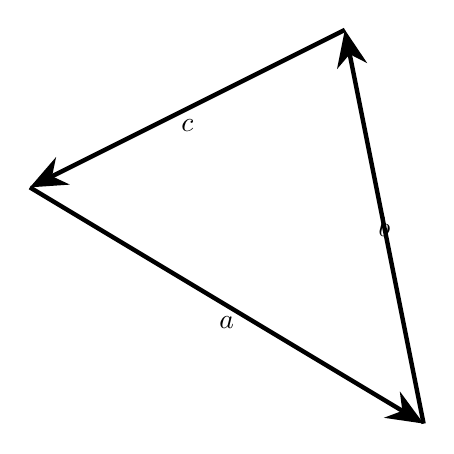
\begin{tikzpicture}
    
    \coordinate (cAPt) at (0,3);
    \coordinate (cBPt) at (5,0);
    \coordinate (cCPt) at (4,5);
    
    \coordinate (cOPt) at (0,0);
    \draw [-{Stealth[scale=1.3,angle'=45]},ultra thick] (cAPt) -- (cBPt) node [midway, below ] {$\lvec{a}$};
    \draw [-{Stealth[scale=1.3,angle'=45]},ultra thick] (cBPt) -- (cCPt) node [midway,  ] {$\lvec{b}$};
    \draw [-{Stealth[scale=1.3,angle'=45]},ultra thick] (cCPt) -- (cAPt) node [midway, below ] {$\lvec{c}$};
   
    \end{tikzpicture}


\begin{tikzpicture}[x={(-.1cm,-.15cm)},y={(1cm,0cm)},z={(0cm,1cm)}]
%正圓錐

\draw[->] (-5,0,0) -- (5,0,0) node[below] {$x$};
\draw[->] (0,-2,0) -- (0,2,0) node[] {$y$};
\draw[->] (0,0,-1) -- (0,0,3) node[above] {$z$};

\draw[color=red] plot[domain=0:2*pi] ({sin(\x r)},{cos(\x r)},2);
\draw[color=red] (0,0,0) -- (0,1,2) (0,0,0) -- (0,-1,2);
\end{tikzpicture}

\begin{tikzpicture}[x={(-.1cm,-.15cm)},y={(1cm,0cm)},z={(0cm,1cm)}]
%正立方體
\draw[->] (-1,0,0) -- (5,0,0) node[below] {$x$};
\draw[->] (0,-2,0) -- (0,2,0) node[] {$y$};
\draw[->] (0,0,-1) -- (0,0,3) node[above] {$z$};
%\draw[color=red] plot[domain=0:2*pi] ({sin(\x r)},{cos(\x r)},2);
\draw[color=red] (0,0,0) -- (1,0,0) -- (1,1,0) -- (0,1,0) -- cycle;

\draw[color=red] (0,0,1) -- (1,0,1) -- (1,1,1) -- (0,1,1) -- cycle;

\draw[color=red] (0,0,0) -- (0,0,1) (1,0,0) -- (1,0,1) (1,1,0) -- (1,1,1) (0,1,0) -- (0,1,1) ;

\end{tikzpicture}

	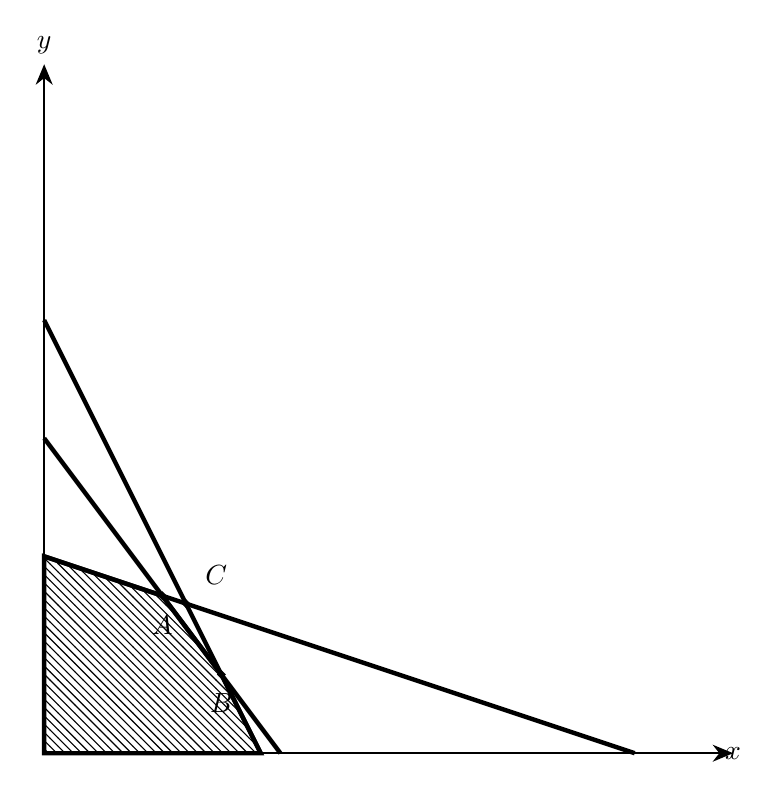
\begin{tikzpicture}[scale=0.25]
    
    \coordinate (cL1XPt) at (12,0);
    \coordinate (cL1YPt) at (0,16);
    \coordinate (cL2XPt) at (30,0);
    \coordinate (cL2YPt) at (0,10);
    \coordinate (cL3XPt) at (11,0);
    \coordinate (cL3YPt) at (0,22);
    
    \coordinate (cOPt) at (0,0);
    \draw [ultra thick] (cL1XPt) -- (cL1YPt);
    \draw [ultra thick] (cL2XPt) -- (cL2YPt);
    \draw [ultra thick] (cL3XPt) -- (cL3YPt);

    \coordinate (cAPt) at (intersection of cL1XPt--cL1YPt and cL2XPt--cL2YPt);
    \coordinate (cBPt) at (intersection of cL1XPt--cL1YPt and cL3XPt--cL3YPt);
    \coordinate (cCPt) at (intersection of cL2XPt--cL2YPt and cL3XPt--cL3YPt);
    
    \draw [ pattern=north west lines, ultra thick] (cOPt) -- (cL3XPt) -- (cBPt) -- (cAPt) -- (cL2YPt) -- cycle ;

    \foreach \v/\u/\t in 
    {cAPt/270/$A$,
     cBPt/270/$B$,
     cCPt/45/$C$
    }
    {
        \draw[ultra thick,fill] (\v) circle (2pt);
        \node[label=\u:\t] at (\v){};
    };
    
    % x軸 y 軸 axes
    \draw[-{Stealth[scale=1.3,angle'=45]},semithick] (0,0) -- (35,0) node[] {$x$};
    \draw[-{Stealth[scale=1.3,angle'=45]},semithick] (0,0) -- (0,35)   node[above] {$y$};

    \end{tikzpicture}


    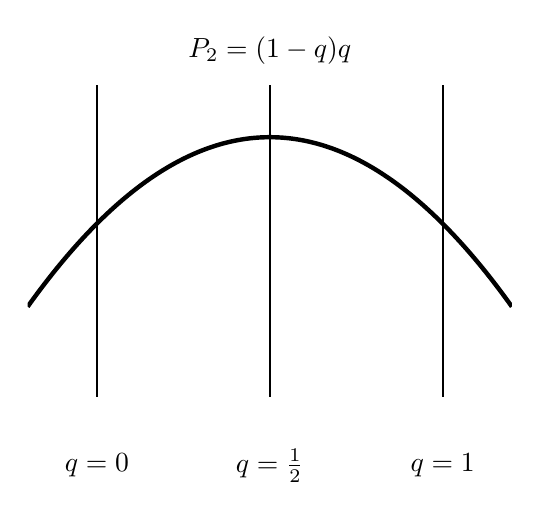
\begin{tikzpicture}[scale=1.0]
    \pgfmathdeclarefunction{polyAAA}{0}{%
       \pgfmathparse{(1-x)*x}%
    }
    
    \begin{axis}[
    unit vector ratio*=1 1 1,
    axis lines = middle,
    axis line style =  {-{Stealth[scale=1.3,angle'=45]}},
    width=11cm,
    xlabel={$x$},
    ylabel={$y$},
    hide y axis,
    hide x axis,
    domain=-0.2:1.2,
    ymin=-1,
    ymax=+0.8,
    xmin=-0.2,
    xmax=+1.2,
    xtick={-1,0,1,2},
    ytick={-1,0,1,2},
    samples=160,
    y tick label style={, xshift=0.25em}
    ]
    \draw[thick] (axis cs:0,-0.5) -- (axis cs:0,0.4);
    \draw[thick] (axis cs:1,-0.5) -- (axis cs:1,0.4);
    \draw[thick] (axis cs:0.5,-0.5) -- (axis cs:0.5,0.4);
    
    \addplot[black,ultra thick,mark=none, domain=-0.2:1.2] {polyAAA} ;
    \node at (axis cs:0, -0.7) {$q=0$};
    \node at (axis cs:1, -0.7) {$q=1$};
    \node at (axis cs:0.5, -0.7) {$q=\frac{1}{2}$};
    \node at (axis cs:0.5, 0.5) {$P_{2}= (1-q) q $};
    
    \end{axis}
    \end{tikzpicture} 
qrt    \newpage
    \tikzset{
        treenode/.style = {shape=rectangle, rounded corners,
            draw, align=center,
            top color=white, bottom color=blue!20},
        root/.style     = {treenode, font=\Large, bottom color=red!30},
        env/.style      = {treenode, font=\ttfamily\normalsize},
        dummy/.style    = {circle,draw}
    }
    
        \begin{tikzpicture}
        [
        grow                    = ,
        %sibling distance        = 5em,
        level 1/.style={sibling distance=20mm},
        level 2/.style={sibling distance=10mm},
        level distance          = 7em,
        edge from parent/.style = {draw, -latex},
        every node/.style       = {font=\footnotesize},
        sloped
        ]
        \node [root] {全班}
        child { node [env] {沒談過}
            child { node [env] {$B$卷}
                edge from parent node [below] {$\frac{1}{4}$} }
            child { node [env] {$A$卷}
                edge from parent node [above, align=center]
                {$\frac{3}{4}$}}
            edge from parent node [above] {$40-p$} }
        child { node [env] {有談過}
            child { node [env] {$B$卷}
                edge from parent node [below] {$\frac{1}{4}$} }
            child { node [env] {$A$卷}
                edge from parent node [above, align=center]
                {$\frac{3}{4}$}}
           edge from parent node [above] {$p$}
             };

        \end{tikzpicture}
        
        \begin{tikzpicture}
        [
        grow                    = ,
        sibling distance        = 6em,
        level distance          = 10em,
        edge from parent/.style = {draw, -latex},
        every node/.style       = {font=\footnotesize},
        sloped
        ]
        \node [root] {不孕症}
        child { node [env] {第二類}
            child { node [env] {無法人工受孕}
                edge from parent node [below] {$1$} }
            edge from parent node [below] {$1-p$} }
        child { node [env] {第一類}
            child { node [env] {人工受孕失敗}
            edge from parent node [below] {$1-q$} }
            child { node [env] {人工受孕成功}
                edge from parent node [above, align=center]
                {$q$}}
            edge from parent node [above] {$p$} };
        \end{tikzpicture}
        
       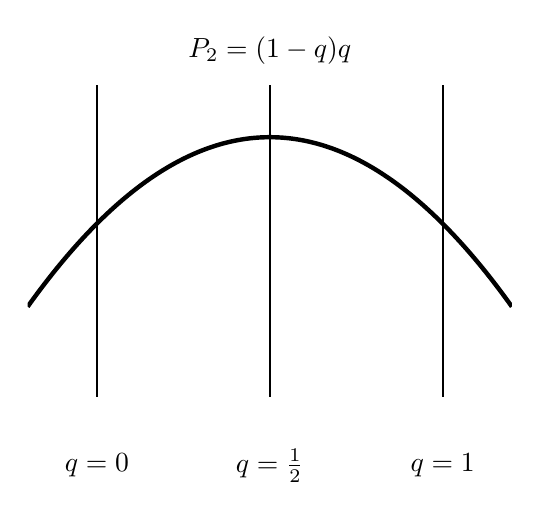
\begin{tikzpicture}[scale=1.0]
       \pgfmathdeclarefunction{polyAAA}{0}{%
           \pgfmathparse{(1-x)*x}%
        }
        \begin{axis}[
        unit vector ratio*=1 1 1,
        axis lines = middle,
        axis line style =  {-{Stealth[scale=1.3,angle'=45]}},
        width=11cm,
        xlabel={$x$},
        ylabel={$y$},
        hide y axis,
        hide x axis,
        domain=-0.2:1.2,
        ymin=-1,
        ymax=+0.8,
        xmin=-0.2,
        xmax=+1.2,
        xtick={-1,0,1,2},
        ytick={-1,0,1,2},
        samples=160,
        y tick label style={, xshift=0.25em}
        ]
        \draw[thick] (axis cs:0,-0.5) -- (axis cs:0,0.4);
        \draw[thick] (axis cs:1,-0.5) -- (axis cs:1,0.4);
        \draw[thick] (axis cs:0.5,-0.5) -- (axis cs:0.5,0.4);
        
        \addplot[black,ultra thick,mark=none, domain=-0.2:1.2] {polyAAA} ;
        \node at (axis cs:0, -0.7) {$q=0$};
        \node at (axis cs:1, -0.7) {$q=1$};
        \node at (axis cs:0.5, -0.7) {$q=\frac{1}{2}$};
        \node at (axis cs:0.5, 0.5) {$P_{2}= (1-q) q $};
        
        \end{axis}
        \end{tikzpicture}    
   \newpage 
   立體圖形
   \\
   四面體
      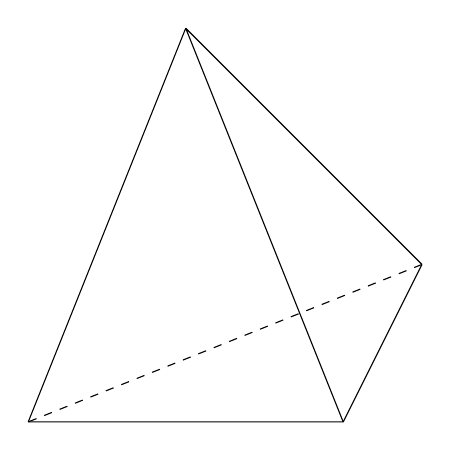
\begin{tikzpicture}      
      %把空間中的四面體利用平面上的替代點來畫圖
      \coordinate (Base1) at (0,0);
      \coordinate (Base2) at (4,0);
      \coordinate (Base3) at (5,2);
      \coordinate (TopPt) at (2,5);
      
      \draw [draw=black, every edge/.append style={draw=black, dashed}]
      (Base1) -- (Base2) --(Base3) 
      (Base3) edge (Base1);
      
      \draw [draw=black, every edge/.append style={draw=black, dashed}]
      (TopPt) -- (Base1) 
      (TopPt) -- (Base2) 
      (TopPt) -- (Base3);
      \end{tikzpicture}
      
            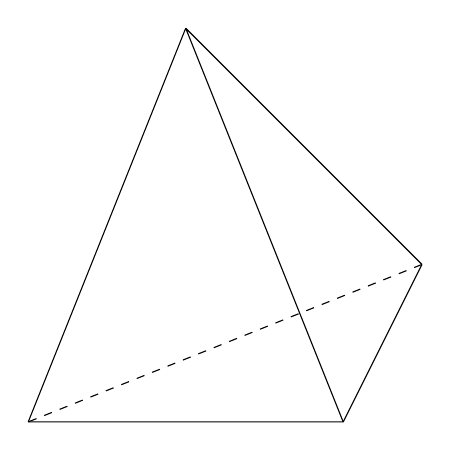
\begin{tikzpicture}      
            %把空間中的四面體利用平面上的替代點來畫圖
            \coordinate (Base1) at (0,0);
            \coordinate (Base2) at (4,0);
            \coordinate (Base3) at (5,2);
            \coordinate (TopPt) at (2,5);
            
            \draw [draw=black, every edge/.append style={draw=black, dashed}]
            (Base1) -- (Base2) --(Base3) 
            (Base3) edge (Base1);
            
            \draw [draw=black, every edge/.append style={draw=black, dashed}]
            (TopPt) -- (Base1) 
            (TopPt) -- (Base2) 
            (TopPt) -- (Base3);
            \end{tikzpicture}
      
        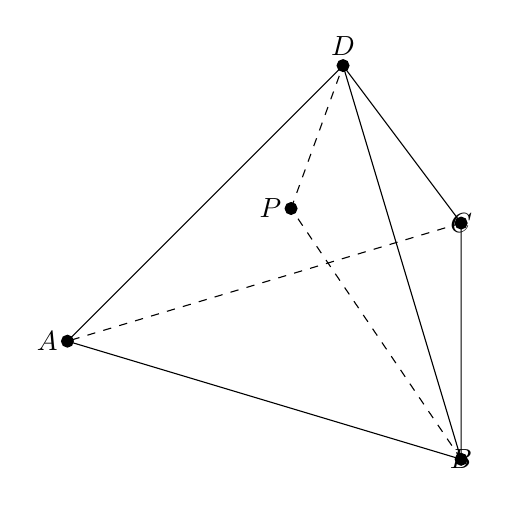
\begin{tikzpicture}      
        %把空間中的四面體利用平面上的替代點來畫圖
        \coordinate (Base1) at (0,0);
        \coordinate (Base2) at (5,-1.5);
        \coordinate (Base3) at (5,1.5);
        \coordinate (TopPt) at (3.5,3.5);
        \coordinate (H) at (3.5,0);
        
        \coordinate (D) at (TopPt);
        \coordinate (A) at (Base1);
        \coordinate (B) at (Base2);
        \coordinate (C) at (Base3);
        \coordinate (M) at ($(A)!0.5!(C)$);
        \coordinate (P) at ($(D)!0.66!(M)$);
        
        \draw [draw=black, every edge/.append style={draw=black, dashed}]
        (Base1) -- (Base2) --(Base3) 
        (Base3) edge (Base1);
        
        \draw [draw=black, every edge/.append style={draw=black, dashed}]
        (TopPt) -- (Base1) 
        (TopPt) -- (Base2) 
        (TopPt) -- (Base3)
        (B) edge (P)
        (P) edge (D);
        
        \foreach \v/\u/\t in 
        { D/above/$D$,
            A/left/$A$,
            B//$B$,
            C//$C$,
            P/left/$P$
        }
        {
            \draw[ultra thick,fill] (\v) circle (1.5pt);
            \node[\u] at (\v){\t};
        }; 
        \end{tikzpicture}

      \begin{tikzpicture}      
      %把空間中的四面體利用平面上的替代點來畫圖
      \coordinate (Base1) at (0,0);
      \coordinate (Base2) at (4,0);
      \coordinate (Base3) at (5,2);
      \coordinate (TopPt) at (2,5);
      
      \coordinate (x) at (6,0);
      
      \coordinate (A) at (TopPt);
      \coordinate (O) at (Base1);
      \coordinate (B) at (Base2);
      \coordinate (C) at (Base3);
      
      \coordinate (M) at ($(B)!0.5!(C)$);
      \coordinate (G) at ($(A)!0.66!(M)$);
      \coordinate (K) at 
      ($(O)!0.66!(B)$);

      \tkzMark(G,K,O)
      \tkzMark(O,G,B)
            
      
      \draw [draw=black, every edge/.append style={draw=black, dashed}]
      (Base1) -- (Base2) --(Base3) 
      (Base3) edge (Base1);
      
      \draw [draw=black, every edge/.append style={draw=black, dashed}]
      (TopPt) -- (Base1) 
      (TopPt) -- (Base2) 
      (TopPt) -- (Base3)
      (A) -- (M)
      (O) edge (G)
      (G) -- (B)
      (G) edge (K);
      
      \draw [-{Stealth[scale=1.3,angle'=45]},semithick] (O) -- (x);
      
      \foreach \v/\u/\t in 
      { A/above/$A$,
          O/left/$O$,
          B/below/$B$,
          C//$C$,
          M//$M$,
          G//$G$,
          K/below/$K$
        }
        {
            \draw[ultra thick,fill] (\v) circle (1.5pt);
            \node[\u] at (\v){\t};
        }; 
        \node[] at (x){$x$};

        \end{tikzpicture}

      \begin{tikzpicture}      
      %把空間中的四面體利用平面上的替代點來畫圖
      \coordinate (Base1) at (0,0);
      \coordinate (Base2) at (4,0);
      \coordinate (Base3) at (5,2);
      \coordinate (TopPt) at (2,5);
      
      \coordinate (A) at (TopPt);
      \coordinate (B) at (Base1);
      \coordinate (C) at (Base2);
      \coordinate (D) at (Base3);
      
      \coordinate (M) at ($(C)!0.5!(D)$);
         
      \draw [draw=black, every edge/.append style={draw=black, dashed}]
      (Base1) -- (Base2) --(Base3) 
      (Base3) edge (Base1);
      
      \draw [draw=black, every edge/.append style={draw=black, dashed}]
      (TopPt) -- (Base1) 
      (TopPt) -- (Base2) 
      (TopPt) -- (Base3);
      
      \draw [ultra thick] (A) -- (M) -- (B)--cycle;
        \foreach \v/\u/\t in 
        { A/above/$A$,
         B/left/$B$,
         C//$C$,
         D//$D$,
         M//$M$
        }
        {
            \draw[ultra thick,fill] (\v) circle (1.5pt);
            \node[\u] at (\v){\t};
        }; 
      \end{tikzpicture}
        \begin{tikzpicture}      
        %把空間中的四面體利用平面上的替代點來畫圖
        \coordinate (Base1) at (0,0);
        \coordinate (Base2) at (5,-1.5);
        \coordinate (Base3) at (5,1.5);
        \coordinate (TopPt) at (3.5,3.5);
        \coordinate (H) at (3.5,0);
        
        \coordinate (O) at (TopPt);
        \coordinate (A) at (Base1);
        \coordinate (B) at (Base2);
        \coordinate (C) at (Base3);
        
        \draw [draw=black, every edge/.append style={draw=black, dashed}]
        (Base1) -- (Base2) --(Base3) 
        (Base3) edge (Base1);
        
        \draw [draw=black, every edge/.append style={draw=black, dashed}]
        (TopPt) -- (Base1) 
        (TopPt) -- (Base2) 
        (TopPt) -- (Base3)
        (TopPt) -- (H);

        \foreach \v/\u/\t in 
        { O/above/$O$,
            A/left/$A$,
            B//$B$,
            C//$C$,
            H//$H$
        }
        {
            \draw[ultra thick,fill] (\v) circle (1.5pt);
            \node[\u] at (\v){\t};
        }; 
        \end{tikzpicture}
        \begin{tikzpicture}      
        %把空間中的四面體利用平面上的替代點來畫圖
        \coordinate (Base1) at (0,0);
        \coordinate (Base2) at (3,-2);
        \coordinate (Base3) at (5,0);
        \coordinate (TopPt) at (2,3.5);
        \coordinate (H) at (2,-0.55);
        
        \coordinate (O) at (TopPt);
        \coordinate (A) at (Base1);
        \coordinate (B) at (Base2);
        \coordinate (C) at (Base3);
        \coordinate (P) at ($(O)!0.3!(A)$);

        
        \draw [draw=black, every edge/.append style={draw=black, dashed}]
        (Base1) -- (Base2) --(Base3) 
        (Base3) edge (Base1);
        
        \draw [draw=black, every edge/.append style={draw=black, dashed}]
        (TopPt) -- (Base1) 
        (TopPt) -- (Base2) 
        (TopPt) -- (Base3)
        (TopPt) -- (H);
        
        %\draw [ultra thick] (A) -- (M) -- (B)--cycle;
        \foreach \v/\u/\t in 
        { O/above/$O$,
            A/left/$A$,
            B//$B$,
            C//$C$,
            H//$H$,
            P/left/$P$
        }
        {
            \draw[ultra thick,fill] (\v) circle (1.5pt);
            \node[\u] at (\v){\t};
        }; 
        \end{tikzpicture}
        
        Test\\
           \begin{tikzpicture}[every edge quotes/.append style={auto, text=blue},z={(0cm,1cm)},y={(1cm,0cm)}, x={(-0.3cm,-0.3cm)}]

           %%空間坐標中的CUBE 是以平面上的x軸 y軸再去擴充出深度z軸 z 往前為正,向後為負
           \coordinate (A) at (0,0,0);
           \coordinate (B) at (0,4,0);
           \coordinate (C) at (2.5,2.8,0);
           
            \coordinate (A1) at (0,0,3);
            \coordinate (B1) at (0,4,3);
            \coordinate (C1) at (2.5,2.8,3);
            
            \coordinate (D) at ($(A1)!0.5!(B1)$);
            \coordinate (E) at ($(A1)!0.5!(C1)$);

           \draw [draw=black, every edge/.append style={draw=black, dashed}]
           (A) edge (B)
           (A)--(C)
           (B)--(C)
           (A1)--(B1)
           (A1)--(C1)
           (B1)--(C1)
           (A) --(A1)
           (B) --(B1)
           (C) --(C1)
           (A) -- (E)
           (B) edge (D);
           
           
           \foreach \v/\u/\t in 
           { A/left/$A$,
               A1/left/$A_1$,
               B//$B$,
               B1//$B_1$,
               C/below left/$C$,
               C1/below left/$C_1$,
               D/above/$D$,
               E/below/$E$
            }
            {
                \draw[ultra thick,fill] (\v) circle (1.5pt);
                \node[\u] at (\v){\t};
            }; 

            \end{tikzpicture}
           \begin{tikzpicture}[every edge quotes/.append style={auto, text=blue},z={(0cm,1cm)},y={(1cm,0cm)}, x={(-0.3cm,-0.5cm)}]
           

           %%空間坐標中的CUBE 是以平面上的x軸 y軸再去擴充出深度z軸 z 往前為正,向後為負
           \coordinate (O) at (0,0,0);
           \coordinate (x) at (7,0,0);
           \coordinate (y) at 
           (0,6,0);
           \coordinate (z) at (0,0,5);
           \coordinate (B) at (6,0,0);
           \coordinate (C) at (3, {sqrt(27)},0);
           \coordinate (M) at ($(O)!0.5!(B)$);
           \coordinate (G) at ($(M)!0.33!(C)$);
           \coordinate (A) at (3, {sqrt(3)}, {sqrt(24)});
           \draw [draw=black, every edge/.append style={draw=black, dashed}]
           (O) edge (A)
           (O) -- (B)
           (O) edge (C)
           (A) -- (B)
           (A) -- (C)
           (B) -- (C)
           (M) edge (C)
           (G) edge (A); 
           \draw [-{Stealth[scale=1.3,angle'=45]},semithick] (O) -- (x);
           \draw [-{Stealth[scale=1.3,angle'=45]},semithick] (O) -- (y);
           \draw [-{Stealth[scale=1.3,angle'=45]},semithick] (O) -- (z);
           
      \foreach \v/\u/\t in 
      { A/above/$A$,
          O/below/$O$,
          B/left/$B$,
          C/below /$C$,
          M/below /$M$,
          G/below /$G$
        }
        {
            \draw[ultra thick,fill] (\v) circle (1.5pt);
            \node[\u] at (\v){\t};
        }; 
        \node[below left] at (x){$x$};
        \node[] at (y){$y$};
        \node[above] at (z){$z$};
        \tkzMark(O,M,C)
        \tkzMark(A,G,C)
           \end{tikzpicture}
   四角錐\\
   \begin{tikzpicture}[every edge quotes/.append style={auto, text=blue},y={(0cm,1cm)},x={(1cm,0cm)}, z={(-0.25cm,-0.5cm)}]
        
       \pgfmathsetmacro{\sizeEdge}{4}
       \pgfmathsetmacro{\sizeEdgeZ}{6}
       
       \pgfmathsetmacro{\sizeHigh}{0.5}

       %%空間坐標中的CUBE 是以平面上的x軸 y軸再去擴充出深度z軸 z 往前為正,向後為負
       \coordinate (Base1) at (0,0,0);
       \coordinate (Base2) at (0,0, \sizeEdgeZ);
       \coordinate (Base3) at (\sizeEdge,0,\sizeEdgeZ);
       \coordinate (Base4) at (\sizeEdge,0,0);
       \coordinate (TopPt) at (0.5 *\sizeEdge, \sizeHigh, 0.5 * \sizeEdgeZ);
       
       \draw [draw=black, every edge/.append style={draw=black, dashed}]
       (Base1) -- (Base2) --(Base3) --(Base4) -- cycle;
       \draw [draw=lightgray, every edge/.append style={draw=black, dashed}]
       (TopPt) -- (Base1) 
       (TopPt) -- (Base2) 
       (TopPt) -- (Base3)
       (TopPt) -- (Base4);
    \end{tikzpicture}
    
       \begin{tikzpicture}[every edge quotes/.append style={auto, text=blue},y={(0cm,1cm)},x={(1cm,0cm)}, z={(-0.25cm,-0.5cm)}]
       
       \pgfmathsetmacro{\sizeEdge}{4}
       \pgfmathsetmacro{\sizeEdgeZ}{6}
       
       \pgfmathsetmacro{\sizeHigh}{0.5}
       
       %%空間坐標中的CUBE 是以平面上的x軸 y軸再去擴充出深度z軸 z 往前為正,向後為負
       \coordinate (Base1) at (0,0,0);
       \coordinate (Base2) at (0,0, \sizeEdgeZ);
       \coordinate (Base3) at (\sizeEdge,0,\sizeEdgeZ);
       \coordinate (Base4) at (\sizeEdge,0,0);
       \coordinate (TopPt) at (0.5 *\sizeEdge, \sizeHigh, 0.5 * \sizeEdgeZ);
       
       
       \coordinate (D) at (Base1); 
       \coordinate (A) at (Base2);
       \coordinate (B) at (Base3);
       \coordinate (C) at (Base4);
       \coordinate (P) at (TopPt);
       
       \coordinate (O) at ($ (A) !0.5! (C)$);
       \coordinate (M) at ($ (B) !0.5! (C)$);
       
       
       \draw [draw=black, every edge/.append style={draw=black, dashed}]
       (Base1) -- (Base2) --(Base3) --(Base4) -- cycle;
       \draw [draw=lightgray, every edge/.append style={draw=black, dashed}]
       (TopPt) -- (Base1) 
       (TopPt) -- (Base2) 
       (TopPt) -- (Base3)
       (TopPt) -- (Base4);
       \draw [draw=black, every edge/.append style={draw=black, dashed}, ultra thick]
       (P) -- (O) -- (M) -- cycle;
       
       
       \foreach \v/\u/\t in 
       { A/left/$A$,
         B//$B$,
         C//$C$,
         D/left/$D$,
         O/below/$O$,
         P/above/$P$,
         M//$M$
        }
        {
            \draw[ultra thick,fill] (\v) circle (1.5pt);
            \node[\u] at (\v){\t};
        };     
       
       \end{tikzpicture}
       
       \begin{tikzpicture}[every edge quotes/.append style={auto, text=blue},y={(0cm,1cm)},x={(1cm,0cm)}, z={(-0.25cm,-0.5cm)}]
       
       \pgfmathsetmacro{\sizeEdge}{4}
       \pgfmathsetmacro{\sizeEdgeZ}{6}
       
       \pgfmathsetmacro{\sizeHigh}{0.5}
       
       %%空間坐標中的CUBE 是以平面上的x軸 y軸再去擴充出深度z軸 z 往前為正,向後為負
       \coordinate (Base1) at (0,0,0);
       \coordinate (Base2) at (0,0, \sizeEdgeZ);
       \coordinate (Base3) at (\sizeEdge,0,\sizeEdgeZ);
       \coordinate (Base4) at (\sizeEdge,0,0);
       \coordinate (TopPt) at (0.5 *\sizeEdge, \sizeHigh, 0.5 * \sizeEdgeZ);
       
       
       \coordinate (D) at (Base1); 
       \coordinate (A) at (Base2);
       \coordinate (B) at (Base3);
       \coordinate (C) at (Base4);
       \coordinate (P) at (TopPt);
       
       \coordinate (O) at ($ (A) !0.5! (C)$);
       \coordinate (M) at ($ (B) !0.5! (C)$);
       \coordinate (N) at ($ (P) !0.75! (B)$);
       
       
       \draw [draw=black, every edge/.append style={draw=black, dashed}]
       (Base1) -- (Base2) --(Base3) --(Base4) -- cycle;
       \draw [draw=lightgray, every edge/.append style={draw=black, dashed}]
       (TopPt) -- (Base1) 
       (TopPt) -- (Base2) 
       (TopPt) -- (Base3)
       (TopPt) -- (Base4);
       \draw [draw=lightgray, every edge/.append style={draw=black, dashed}, thick]
       (P) -- (O) -- (M) -- cycle;
       
       \draw [draw=black, every edge/.append style={draw=black, dashed}, ultra thick]
       (N) -- (A) -- (C) -- cycle;
       
       \foreach \v/\u/\t in 
       { A/left/$A$,
           B//$B$,
           C//$C$,
           D/left/$D$,
           O/below/$O$,
           P/above/$P$,
           M//$M$,
           N//$N$
        }
        {
            \draw[ultra thick,fill] (\v) circle (1.5pt);
            \node[\u] at (\v){\t};
        };     
        
        \end{tikzpicture}
    \begin{tikzpicture}[every edge quotes/.append style={auto, text=blue}]
    \pgfmathsetmacro{\cubex}{3}
    \pgfmathsetmacro{\cubey}{4}
    \pgfmathsetmacro{\cubez}{5}
    %%空間坐標中的CUBE 是以平面上的x軸 y軸再去擴充出深度z軸 z 往前為正,向後為負
    \coordinate (A) at (0,0,0);
    \coordinate (B) at (0,0,\cubez);
    
    \coordinate (Bout) at (0,0,1.5*\cubez);
    
    \coordinate (C) at (\cubex, 0, \cubez );
    \coordinate (D) at (\cubex,0,0);
    
    \coordinate (Dout) at (1.5*\cubex, 0, 0);
    
    \coordinate (E) at (0, -\cubey, 0);
    
    \coordinate (Eout) at (0, -\cubey *1.8, 0) ;
    
    \coordinate (F) at (0, -\cubey, \cubez);
    \coordinate (G) at (\cubex, -\cubey, \cubez);
    \coordinate (H) at (\cubex, -\cubey, 0); 
    
    \draw [draw=black, every edge/.append style={draw=black, dashed}]
    (A) -- (B) --(C) --(D) -- cycle
    (C) -- (G) -- (H) -- (D) --cycle
    (B) -- (F) -- (G) -- (C) --cycle 
    (A) edge (E) 
    (E) edge (H)
    (E) edge (F);
    
    \draw [fill=lightgray, opacity=0.5] (B)--(G)--(D) -- cycle;
    
    \draw[-{Stealth[scale=1.3,angle'=45]}, ultra thick] (A) -- (Dout) node[] {$y$};
    \draw[-{Stealth[scale=1.3,angle'=45]}, ultra thick] (A) -- (Bout) node[below] {$x$};
    \draw[-{Stealth[scale=1.3,angle'=45]}, ultra thick] (A) -- (Eout) node[below] {$z$};
    \foreach \v/\u/\t in 
    {C//$C$,
        F/left/$F$,
        H//$H$
    }
    {
        \draw[ultra thick,fill] (\v) circle (2.5pt);
        \node[\u] at (\v){\t};
    };     
    \draw[ultra thick,fill] (A) circle (2.5pt);
    \draw[ultra thick,fill] (B) circle (2.5pt);
    \draw[ultra thick,fill] (D) circle (2.5pt);
    \draw[ultra thick,fill] (E) circle (2.5pt);
    \draw[ultra thick,fill] (G) circle (2.5pt);
    
    \node[above] at (A){$A(0,0,0)$};
    \node[label={[shift={(-1,0)}]$B(1,0,0)$} ] at (B) {};
    \node[above] at (D){$D(0,1,0)$};
    \node[] at (G){$G(1,1,1)$};
    \node[label={[shift={(-1,0)}]$E(0,0,1)$}] at (E){};
    
    \end{tikzpicture}
    \begin{tikzpicture}[every edge quotes/.append style={auto, text=blue}]
    \pgfmathsetmacro{\cubex}{3}
    \pgfmathsetmacro{\cubey}{4}
    \pgfmathsetmacro{\cubez}{5}
    %%空間坐標中的CUBE 是以平面上的x軸 y軸再去擴充出深度z軸 z 往前為正,向後為負
    \coordinate (A) at (0,0,0);
    \coordinate (B) at (0,0,\cubez);
    
    \coordinate (Bout) at (0,0,1.5*\cubez);
    
    \coordinate (C) at (\cubex, 0, \cubez );
    \coordinate (D) at (\cubex,0,0);
    
    \coordinate (Dout) at (1.5*\cubex, 0, 0);
    
    \coordinate (E) at (0, -\cubey, 0);
    
    \coordinate (Eout) at (0, -\cubey *1.8, 0) ;
    
    \coordinate (F) at (0, -\cubey, \cubez);
    \coordinate (G) at (\cubex, -\cubey, \cubez);
    \coordinate (H) at (\cubex, -\cubey, 0); 
    
    \draw [draw=black, every edge/.append style={draw=black, dashed}]
    (A) -- (B) --(C) --(D) -- cycle
    (C) -- (G) -- (H) -- (D) --cycle
    (B) -- (F) -- (G) -- (C) --cycle 
    (A) edge (E) 
    (E) edge (H)
    (E) edge (F);
    
    \draw [fill,pattern=north west lines] (B)--(G)--(D) -- cycle;
    
    \draw[-{Stealth[scale=1.3,angle'=45]}, ultra thick] (A) -- (Dout) node[] {$y$};
    \draw[-{Stealth[scale=1.3,angle'=45]}, ultra thick] (A) -- (Bout) node[below] {$x$};
    \draw[-{Stealth[scale=1.3,angle'=45]}, ultra thick] (A) -- (Eout) node[below] {$z$};
    \foreach \v/\u/\t in 
    {C/above/$C$,
        F/left/$F$,
        G//$G$,
        H//$H$
    }
    {
        \draw[ultra thick,fill] (\v) circle (2.5pt);
        \node[\u] at (\v){\t};
    };     
    \draw[ultra thick,fill] (A) circle (2.5pt);
    \draw[ultra thick,fill] (B) circle (2.5pt);
    \draw[ultra thick,fill] (D) circle (2.5pt);
    \draw[ultra thick,fill] (E) circle (2.5pt);
    
    
    
    \node[above] at (A){$A(0,0,0)$};
    \node[label={[shift={(-1,0)}]$B(1,0,0)$} ] at (B) {};
    \node[above] at (D){$D(0,1,0)$};
    \node[label={[shift={(-1,0)}]$E(0,0,1)$}] at (E){};
    
    \end{tikzpicture}
    \begin{tikzpicture}[every edge quotes/.append style={auto, text=blue}]
    \pgfmathsetmacro{\cubex}{3}
    \pgfmathsetmacro{\cubey}{4}
    \pgfmathsetmacro{\cubez}{5}
    %%空間坐標中的CUBE 是以平面上的x軸 y軸再去擴充出深度z軸 z 往前為正,向後為負
    \coordinate (A) at (0,0,0);
    \coordinate (B) at (0,0,\cubez);
    
    \coordinate (Bout) at (0,0,1.5*\cubez);
    
    \coordinate (C) at (\cubex, 0, \cubez );
    \coordinate (D) at (\cubex,0,0);
    
    \coordinate (Dout) at (1.5*\cubex, 0, 0);
    
    \coordinate (E) at (0, -\cubey, 0);
    
    \coordinate (Eout) at (0, -\cubey *1.8, 0) ;
    
    \coordinate (F) at (0, -\cubey, \cubez);
    \coordinate (G) at (\cubex, -\cubey, \cubez);
    \coordinate (H) at (\cubex, -\cubey, 0); 
    
    \draw [draw=black, every edge/.append style={draw=black, dashed}]
    (A) -- (B) --(C) --(D) -- cycle
    (C) -- (G) -- (H) -- (D) --cycle
    (B) -- (F) -- (G) -- (C) --cycle 
    (A) edge (E) 
    (E) edge (H)
    (E) edge (F);
    
    
    \draw[-{Stealth[scale=1.3,angle'=45]}, ultra thick] (A) -- (Dout) node[] {$y$};
    \draw[-{Stealth[scale=1.3,angle'=45]}, ultra thick] (A) -- (Bout) node[below] {$x$};
    \draw[-{Stealth[scale=1.3,angle'=45]}, ultra thick] (A) -- (Eout) node[below] {$z$};
    \foreach \v/\u/\t in 
    {C/above/$C$,
        F/left/$F$,
        G//$G$,
        H//$H$
    }
    {
        \draw[ultra thick,fill] (\v) circle (2.5pt);
        \node[\u] at (\v){\t};
    };     
    \draw[ultra thick,fill] (A) circle (2.5pt);
    \draw[ultra thick,fill] (B) circle (2.5pt);
    \draw[ultra thick,fill] (D) circle (2.5pt);
    \draw[ultra thick,fill] (E) circle (2.5pt);
    
    
    
    \node[above] at (A){$A(0,0,0)$};
    \node[label={[shift={(-1,0)}]$B(1,0,0)$} ] at (B) {};
    \node[above] at (D){$D(0,1,0)$};
    \node[label={[shift={(-1,0)}]$E(0,0,1)$}] at (E){};
    
    \end{tikzpicture}
    \begin{tikzpicture}[every edge quotes/.append style={auto, text=blue}]
    \pgfmathsetmacro{\cubex}{3}
    \pgfmathsetmacro{\cubey}{3}
    \pgfmathsetmacro{\cubez}{3}
    
    \pgfmathsetmacro{\cubeShiftX}{0} %做出平行六面體的傾斜感
    %%空間坐標中的CUBE 是以平面上的x軸 y軸再去擴充出深度z軸 z 往前為正,向後為負
    \coordinate (Eup1) at (0,0,0);
    \coordinate (Eup2) at (0,0,\cubez);
    \coordinate (Eup3) at (\cubex, 0, \cubez );
    \coordinate (Eup4) at (\cubex,0,0);
    \coordinate (Ecenter) at (0.5*\cubex , 0,0.5*\cubez);
    \coordinate (Edown1) at (\cubeShiftX+0, -\cubey, 0);
    \coordinate (Edown2) at (\cubeShiftX+0, -\cubey, \cubez);
    \coordinate (Edown3) at (\cubeShiftX+\cubex, -\cubey, \cubez);
    \coordinate (Edown4) at (\cubeShiftX+\cubex, -\cubey, 0); 
    \draw [draw=black, every edge/.append style={draw=black, dashed}]
    (Eup1) -- (Eup2) --(Eup3) --(Eup4) -- cycle
    (Eup3) -- (Edown3) -- (Edown4) -- (Eup4) --cycle
    (Eup2) -- (Edown2) -- (Edown3) -- (Eup3) --cycle 
    (Eup1) edge (Edown1) 
    (Edown1) edge (Edown4)
    (Edown1) edge (Edown2);
    
    \foreach \v/\u/\t in 
    {Eup1/180/$D$,
        Eup2/180/$A$,
        Eup3/0/$B$,
        Eup4/0/$C$,
        Edown1/180/$H$,
        Edown2/180/$E$,
        Edown3/0/$F$,
        Edown4/0/$G$,
        Ecenter/0/$K$
    }
    {
        \draw[ultra thick,fill] (\v) circle (2.5pt);
        \node[label=\u:\t] at (\v){};
    };     
    \end{tikzpicture}
    
    \begin{tikzpicture}[every edge quotes/.append style={auto, text=blue}]
    \pgfmathsetmacro{\cubex}{4}
    \pgfmathsetmacro{\cubey}{2}
    \pgfmathsetmacro{\cubez}{6}
    
    \pgfmathsetmacro{\cubeShiftX}{0} %做出平行六面體的傾斜感
    %%空間坐標中的CUBE 是以平面上的x軸 y軸再去擴充出深度z軸 z 往前為正,向後為負
    \coordinate (Eup1) at (0,0,0);
    \coordinate (Eup2) at (0,0,\cubez);
    \coordinate (Eup3) at (\cubex, 0, \cubez );
    \coordinate (Eup4) at (\cubex,0,0);
    \coordinate (Edown1) at (\cubeShiftX+0, -\cubey, 0);
    \coordinate (Edown2) at (\cubeShiftX+0, -\cubey, \cubez);
    \coordinate (Edown3) at (\cubeShiftX+\cubex, -\cubey, \cubez);
    \coordinate (Edown4) at (\cubeShiftX+\cubex, -\cubey, 0); 
    \draw [draw=black, every edge/.append style={draw=black, dashed}]
    (Eup1) -- (Eup2) --(Eup3) --(Eup4) -- cycle
    (Eup3) -- (Edown3) -- (Edown4) -- (Eup4) --cycle
    (Eup2) -- (Edown2) -- (Edown3) -- (Eup3) --cycle 
    (Eup1) edge (Edown1) 
    (Edown1) edge (Edown4)
    (Edown1) edge (Edown2);
    
    \foreach \v/\u/\t in 
    {Eup1/180/$H$,
        Eup2/180/$E$,
        Eup3/0/$F$,
        Eup4/0/$G$,
        Edown1/180/$D$,
        Edown2/180/$A$,
        Edown3/0/$B$,
        Edown4/0/$C$
    }
    {
        \draw[ultra thick,fill] (\v) circle (2.5pt);
        \node[label=\u:\t] at (\v){};
    };     
    \end{tikzpicture}
    
        \begin{tikzpicture}[every edge quotes/.append style={auto, text=blue}]
        \pgfmathsetmacro{\cubex}{3}
        \pgfmathsetmacro{\cubey}{3}
        \pgfmathsetmacro{\cubez}{3}
        
        \pgfmathsetmacro{\cubeShiftX}{0} %做出平行六面體的傾斜感
        %%空間坐標中的CUBE 是以平面上的x軸 y軸再去擴充出深度z軸 z 往前為正,向後為負
        \coordinate (Eup1) at (0,0,0);
        \coordinate (Eup2) at (0,0,\cubez);
        \coordinate (Eup3) at (\cubex, 0, \cubez );
        \coordinate (Eup4) at (\cubex,0,0);
        \coordinate (Edown1) at (\cubeShiftX+0, -\cubey, 0);
        \coordinate (Edown2) at (\cubeShiftX+0, -\cubey, \cubez);
        \coordinate (Edown3) at (\cubeShiftX+\cubex, -\cubey, \cubez);
        \coordinate (Edown4) at (\cubeShiftX+\cubex, -\cubey, 0); 
        \draw [draw=black, every edge/.append style={draw=black, dashed}]
        (Eup1) -- (Eup2) --(Eup3) --(Eup4) -- cycle
        (Eup3) -- (Edown3) -- (Edown4) -- (Eup4) --cycle
        (Eup2) -- (Edown2) -- (Edown3) -- (Eup3) --cycle 
        (Eup1) edge (Edown1) 
        (Edown1) edge (Edown4)
        (Edown1) edge (Edown2);
        
        \foreach \v/\u/\t in 
        {Eup1/180/$D$,
            Eup2/180/$A$,
            Eup3/0/$B$,
            Eup4/0/$C$,
            Edown1/180/$H$,
            Edown2/180/$E$,
            Edown3/0/$F$,
            Edown4/0/$G$
        }
        {
            \draw[ultra thick,fill] (\v) circle (2.5pt);
            \node[label=\u:\t] at (\v){};
        };     
        \end{tikzpicture}
    \begin{tikzpicture}[every edge quotes/.append style={auto, text=blue}]
    \pgfmathsetmacro{\cubex}{3.5}
    \pgfmathsetmacro{\cubey}{2}
    \pgfmathsetmacro{\cubez}{3.5}
    
    \pgfmathsetmacro{\cubeShiftX}{-0.5} %做出平行六面體的傾斜感
    %%空間坐標中的CUBE 是以平面上的x軸 y軸再去擴充出深度z軸 z 往前為正,向後為負
    \coordinate (Eup1) at (0,0,0);
    \coordinate (Eup2) at (0,0,\cubez);
    \coordinate (Eup3) at (\cubex, 0, \cubez );
    \coordinate (Eup4) at (\cubex,0,0);
    \coordinate (Edown1) at (\cubeShiftX+0, -\cubey, 0);
    \coordinate (Edown2) at (\cubeShiftX+0, -\cubey, \cubez);
    \coordinate (Edown3) at (\cubeShiftX+\cubex, -\cubey, \cubez);
    \coordinate (Edown4) at (\cubeShiftX+\cubex, -\cubey, 0); 
    \draw [draw=black, every edge/.append style={draw=black, dashed}]
    (Eup1) -- (Eup2) --(Eup3) --(Eup4) -- cycle
    (Eup3) -- (Edown3) -- (Edown4) -- (Eup4) --cycle
    (Eup2) -- (Edown2) -- (Edown3) -- (Eup3) --cycle 
    (Eup1) edge (Edown1) 
    (Edown1) edge (Edown4)
    (Edown1) edge (Edown2);
    
    \foreach \v/\u/\t in 
    {Eup1/180/$H$,
        Eup2/180/$E$,
        Eup3/0/$F$,
        Eup4/0/$G$,
        Edown1/180/$D$,
        Edown2/180/$A$,
        Edown3/0/$B$,
        Edown4/0/$C$
    }
    {
        \draw[ultra thick,fill] (\v) circle (2.5pt);
        \node[label=\u:\t] at (\v){};
    };     
    \end{tikzpicture}
      \begin{tikzpicture}[scale=0.6]
      \pgfmathsetmacro{\EAlphaVectorX}{8}
      \pgfmathsetmacro{\EAlphaVectorY}{0}
      \pgfmathsetmacro{\EBetaVectorX}{2}
      \pgfmathsetmacro{\EBetaVectorY}{3}
      \coordinate (cOPt) at (0,0);
      \coordinate (cPPt) at (3,1.5);
      \coordinate (cQPt) at (8,1.5);
      \coordinate (cVectorPP) at (0,3);
      \coordinate (cNVector) at (0,3); 
      \coordinate (cPPrimePt) at ($(cPPt)+(cVectorPP)$);
      \coordinate (cQPrimePt) at ($(cQPt)+(cVectorPP)$);
      \coordinate (cNVectorStartPt) at (1.5,1.5);
      \coordinate (cNVectorEndPt) at ($(cNVectorStartPt) + (cNVector)$);
      \coordinate (cLineStartPt) at (7,4);
      \coordinate (cLineVector) at (-2,-2.5);
      
      \coordinate (cAlphaPt) at  (\EAlphaVectorX, \EAlphaVectorY) ; 
      \coordinate (cLineEndPt) at ($(cLineStartPt) + 2*(cLineVector)$);
      \coordinate (cLineMidPt) at (intersection of cLineStartPt--cLineEndPt and cPPt--cQPt);
      \coordinate (cLineMidPt2) at (intersection of cLineStartPt--cLineEndPt and cOPt--cAlphaPt);
      

      \draw[ultra thick] (cPPt)--(cQPt);
      \draw (cPPrimePt)--(cQPrimePt);
      \draw[fill=lightgray] (cPPt)--(cQPt)--(cQPrimePt)--(cPPrimePt)--cycle;
      \draw (0,0) -- ++(\EAlphaVectorX, \EAlphaVectorY) -- ++(\EBetaVectorX, \EBetaVectorY) -- ++(-\EAlphaVectorX, -\EAlphaVectorY) -- ++(-\EBetaVectorX, -\EBetaVectorY) -- cycle;
      \draw (cPPt) -- ++(cVectorPP);
      \draw (cQPt) -- ++(cVectorPP) ;
      
      \draw[-{Stealth[scale=1.3,angle'=45]},semithick] (cNVectorStartPt) -- (cNVectorEndPt) ;
      
      \draw[ultra thick] (cLineStartPt)--(cLineMidPt);
      \draw[ultra thick,dashed] (cLineMidPt)--(cLineMidPt2);
      \draw[ultra thick] (cLineMidPt2)--(cLineEndPt);
      \foreach \v/\u/\t in 
      { cNVectorEndPt/90/$\lvec{n}$,
        cLineStartPt/180/$\Gamma$,
        cQPrimePt/0/$E_2$
        }
        {
            %\draw[ultra thick,fill] (\v) circle (2.5pt);
            \node[label=\u:\t] at (\v){};
        };
        \draw[ultra thick,fill] (cLineMidPt) circle (2.5pt);
        \node[below] at (8,0){$E_{xy}$};
        %       
        \end{tikzpicture}

   \begin{tikzpicture}[scale=0.6]
       \pgfmathsetmacro{\EAlphaVectorX}{8}
       \pgfmathsetmacro{\EAlphaVectorY}{0}
       \pgfmathsetmacro{\EBetaVectorX}{2}
       \pgfmathsetmacro{\EBetaVectorY}{3}

       \coordinate (cPPt) at (2.5,1.5);
       \coordinate (cQPt) at (7,1.5);
       \coordinate (cVectorPP) at (4,4);
       \coordinate (cNVector) at (0,5); 
       \coordinate (cPPrimePt) at ($(cPPt)+(cVectorPP)$);
       \coordinate (cQPrimePt) at ($(cQPt)+(cVectorPP)$);
       \coordinate (cNVectorEndPt) at ($(cPPt) + (cNVector)$);

       \draw (cPPt)--(cQPt)  node [midway, below ] {$7$};
       \draw (cPPrimePt)--(cQPrimePt);
       \draw[fill=lightgray] (cPPt)--(cQPt)--(cQPrimePt)--(cPPrimePt)--cycle;
       \draw (0,0) -- ++(\EAlphaVectorX, \EAlphaVectorY) -- ++(\EBetaVectorX, \EBetaVectorY) -- ++(-\EAlphaVectorX, -\EAlphaVectorY) -- ++(-\EBetaVectorX, -\EBetaVectorY) -- cycle;
       \draw[-{Stealth[scale=1.3,angle'=45]},semithick] (cPPt) -- ++(cVectorPP);
       \draw[-{Stealth[scale=1.3,angle'=45]},semithick] (cQPt) -- ++(cVectorPP) ;
       \draw[-{Stealth[scale=1.3,angle'=45]},semithick] (cPPt) -- (cNVectorEndPt) ;
       
           \foreach \v/\u/\t in 
           {cPPt/270/$P$,
               cQPt/270/$Q$,
               cPPrimePt/90/$P^\prime$,
               cQPrimePt/90/$Q^\prime$,
               cNVectorEndPt/90/$\lvec{n}$
            }
            {
                %\draw[ultra thick,fill] (\v) circle (2.5pt);
                \node[label=\u:\t] at (\v){};
            };
       \node[below] at (4,0){$E:3x-2y-2z=1$};
%       
   \end{tikzpicture}
   
   \newpage
   \begin{tikzpicture}[scale=1.0]
   \pgfmathdeclarefunction{polyAAA}{0}{%
       \pgfmathparse{ln(x+1)/ln(0.5)+0.5}%
    }
   \pgfmathdeclarefunction{polyBBB}{0}{%
           \pgfmathparse{ln(x+1)/ln(0.5)}%
        }
   
   \pgfmathdeclarefunction{polyori}{0}{%
       \pgfmathparse{ln(x)/ln(0.5)}%
    }
    \begin{axis}[
    unit vector ratio*=1 1 1,
    axis lines = middle,
    axis line style =  {-{Stealth[scale=1.3,angle'=45]}},
    width=11cm,
    xlabel={$x$},
    ylabel={$y$},
    domain=-2:14,
    ymin=-2,
    ymax=+3,
    xmin=-1.5,
    xmax=+3,
    xtick={-1,0,1,2},
    ytick={-1,0,1,2},
    samples=160,
    y tick label style={, xshift=0.25em}
    ]
    \draw[thick] (axis cs:-1,-1) -- (axis cs:-1,3);
    \draw[line width=2.3pt,-{Stealth[scale=1.3,angle'=45]}] (axis cs:1,0 ) -- (axis cs:0,0);
    \draw[line width=2.3pt,-{Stealth[scale=1.3,angle'=45]}] (axis cs:0,0 ) -- (axis cs:0,0.5);
    
    \addplot[black,ultra thick,dashed,mark=none,domain=-0.9:2] {polyBBB} ;
    \addplot[black,ultra thick,mark=none, domain=-0.9:2] {polyAAA} ;
    
    \addplot[black,ultra thick,dotted,mark=none, domain=-0.9:3] {polyori} ;

    \node at (axis cs:-1, -1.5) {$x=-1$};
    \node at (axis cs:1, 2) {$y=\log_b x$};
        \node at (axis cs:1.5, -1.7) {$y=\log_b (x+1)$};
    \end{axis}
    \end{tikzpicture}    

    \begin{tikzpicture}[scale=1.0]
        \pgfmathdeclarefunction{polyAAA}{0}{%
            \pgfmathparse{ln(x+1)/ln(0.5)+0.5}%
        }
    \begin{axis}[
    unit vector ratio*=1 1 1,
    axis lines = middle,
    axis line style =  {-{Stealth[scale=1.3,angle'=45]}},
    width=11cm,
    xlabel={$x$},
    ylabel={$y$},
    domain=-2:14,
    ymin=-2,
    ymax=+3,
    xmin=-1.5,
    xmax=+3,
    xtick={-1,0,1,2},
    ytick={-1,0,1,2},
    samples=160,
    stack plots=y,
    y tick label style={, xshift=0.25em}
    ]
    \draw[thick] (axis cs:-1,-1) -- (axis cs:-1,3);
    
    \addplot+[black,ultra thick,mark=none,stack plots=y, domain=-0.9:3] {polyAAA};
    \node at (axis cs:-1, -1.5) {$x=-1$};

    \end{axis}
    \end{tikzpicture}
    
    \begin{tikzpicture}
    
    \draw [ultra thick](0.5,0) -- (4.5,0);
    
    \draw[ultra thick] (1,0) circle (2pt);
    \draw[ultra thick] (2,0) circle (2pt);
    \draw[ultra thick] (3,0) circle (2pt);
    \draw[ultra thick] (4,0) circle (2pt);
    \draw[ultra thick] (1.5,1.5) circle (2pt);
    \draw[ultra thick] (3.5,1) circle (2pt);
    \end{tikzpicture}
    
    \begin{tikzpicture}[scale=1.5]
    \coordinate (cOPt) at (0:0);
%    \coordinate (cAPt) at (0:1);
%    \coordinate (cBPt) at (56:1);	%粗略B值
%    \coordinate (cCPt) at (112:1);	%粗略C值
    \coordinate (cPPt) at (1,-1);
    \coordinate (cQPt) at (-1.37,-0.37);
    \coordinate (cRPt) at (0.37,1.37);
    \coordinate (cHPt) at (-0.5,0.5);
%H = (-0.5, 0.5)
%P = (1, -1)
%Q = (-1.37, -0.37)
%R = (0.37, 1.37)

    \draw [ultra thick](cPPt) --(cQPt) -- (cRPt) -- (cPPt) circle;

    \draw [ultra thick](cPPt) --(cHPt) ;
    \draw [ultra thick](cOPt) --(cRPt) ;

    \draw[ultra thick] (cPPt) circle (1pt);
    \draw[ultra thick] (cQPt) circle (1pt);
    \draw[ultra thick] (cRPt) circle (1pt);
    
    \draw[domain=-1.7:0.7,smooth,variable=\x,ultra thick] plot ({\x},{\x+1});
    
    \draw[ultra thick] (0,0) circle ({sqrt(2)});

    \node[label=225:$O$] at (cOPt){};
    \node[label=0:$P$] at (cPPt){};
    \node[label=180:$Q$] at (cQPt){};
    \node[label=90:$R$] at (cRPt){};
    \node[label=135:$H$] at (cHPt){};
    \node at (1.8,1.6){$x-y+1=0$};

    % x軸 y 軸 axes
    \draw[-{Stealth[scale=1.3,angle'=45]},semithick] (-2,0) -- (2,0) node[] {$x$};
    \draw[-{Stealth[scale=1.3,angle'=45]},semithick] (0,-2)->(0,2)   node[above] {$y$};
    \end{tikzpicture}
    
	\begin{tikzpicture}
    \newcommand{\BX}{-4};
    \newcommand{\BY}{-4};
    \newcommand{\CX}{2};
    \newcommand{\CY}{-4};
    \coordinate (cAPt) at (0,0);
    \coordinate (cBPt) at (\BX, \BY);
    \coordinate (cCPt) at (\CX, \CY);

    \draw (cAPt) --(cBPt) -- (cCPt) -- (cAPt) circle;
	\draw[-{Stealth[scale=1.3,angle'=45]}, ultra thick] (cAPt) -- (cBPt);
	\draw[-{Stealth[scale=1.3,angle'=45]}, ultra thick] (cAPt) -- (cCPt);
    
    \foreach \v/\u/\t in 
    {cAPt/90/$A$,
        cBPt/180/$B$,
        cCPt/0/$C$
    }
    {
        \draw[ultra thick,fill] (\v) circle (2.5pt);
        \node[label=\u:\t] at (\v){};
    };
    \end{tikzpicture}


        \pgfmathdeclarefunction{polyB}{0}{%
            \pgfmathparse{ln(x+2)/ln(2)}%
        }
        \begin{tikzpicture}[scale=0.6]
        \begin{axis}[
        unit vector ratio*=1 1 1,
        axis lines = middle,
        axis line style =  {-{Stealth[scale=1.3,angle'=45]}},
        width=11cm,
        xlabel={$x$},
        ylabel={$y$},
        domain=-2:14,
        ymin=-2,
        ymax=10,
        xmin=-2,
        xmax=14,
        xtick={-1,0,...,13},
        ytick={-1,0,...,9},
        samples=160,
        stack plots=y
        ]
        \newcommand{\nStartX}{1}
        \newcommand{\nEndX}{8}
        \draw[ultra thick] (axis cs:\nStartX,0) -- (axis cs:\nStartX,8);
        \draw[ultra thick] (axis cs:\nEndX,0) -- (axis cs:\nEndX,8);
        \draw[ultra thick] (axis cs:-5,0) -- (axis cs:12,0);
        
        \addplot+[black,thick,mark=none,stack plots=y, domain=\nStartX:\nEndX] {polyB};
        \addplot+[mark=none,fill=gray!20,draw=black,domain=\nStartX:\nEndX,stack plots=y] {min(0-(polyB),0)} \closedcycle;
        
        \addplot+[black,thick,mark=none,stack plots=y, domain=-1.9:11] {polyB};
        \node at (axis cs:12,4.5){ $\log_2 (x+2)$};
        \node at (axis cs:\nStartX, 9) {$x=1$};
        \node at (axis cs:\nEndX, 9) {$x=8$};
        \node at (axis cs:6, -1.4) {圖一 $B$ 區域};
        \end{axis}
        \end{tikzpicture}
    \pgfmathdeclarefunction{poly}{0}{%
        \pgfmathparse{ln(x)/ln(2)}%
    }
    \begin{tikzpicture}[scale=0.6]
    \begin{axis}[
    unit vector ratio*=1 1 1,
    axis lines = middle,
    axis line style =  {-{Stealth[scale=1.3,angle'=45]}},
    width=11cm,
    %xlabel={$x$},
    %ylabel={$y$},
    domain=-2:14,
    ymin=-2,
    ymax=10,
    xmin=-2,
    xmax=14,
    xtick={-1,0,...,13},
    ytick={-1,0,...,9},
    samples=160,
    stack plots=y
    ]
    \newcommand{\nStartX}{3}
    \newcommand{\nEndX}{10}
    
    
    \draw[ultra thick] (axis cs:\nStartX,0) -- (axis cs:\nStartX,8);
    \draw[ultra thick] (axis cs:\nEndX,0) -- (axis cs:\nEndX,8);
    
    %畫 log 曲線與著色
    \addplot+[black,thick,mark=none,stack plots=y, domain=\nStartX:\nEndX] {poly};
    \addplot+[mark=none,fill=gray!20,draw=black,domain=\nStartX:\nEndX,stack plots=y] {min(0-(poly),0)} \closedcycle;
    % 加強延伸 log f曲線部分
    \addplot+[black,thick,mark=none,stack plots=y, domain=0.1:11] {poly};

    \node at (axis cs:\nStartX, 9) {$x=3$};
    \node at (axis cs:\nEndX, 9) {$x=10$};

    \node at (axis cs:12,3.5){ $\log_2 x$};
    \node at (axis cs:6, -1.4) {圖二};
    \end{axis}
    \end{tikzpicture}
    \pgfmathdeclarefunction{polyA}{0}{%
        \pgfmathparse{ln(x)/ln(2)+5}%
    }
    \begin{tikzpicture}[scale=0.6]
        \begin{axis}[
        unit vector ratio*=1 1 1,
        axis lines = middle,
        axis line style = {-{Stealth[scale=1.3,angle'=45]}},
        width=11cm,
        %xlabel={$x$},
        %ylabel={$y$},
        domain=-2:14,
        ymin=-2,
        ymax=10,
        xmin=-2,
        xmax=14,
        xtick={-1,0,...,13},
        ytick={-1,0,...,9},
        samples=160,
        stack plots=y
        ]
        \newcommand{\nStartX}{3}
        \newcommand{\nEndX}{10}

        \draw[ultra thick] (axis cs:\nStartX,0) -- (axis cs:\nStartX,8);
        \draw[ultra thick] (axis cs:\nEndX,0) -- (axis cs:\nEndX,8.5);
        
        \draw[ultra thick] (axis cs:0.5,5) -- (axis cs:12,5);
       
        \draw [ pattern=north west lines, ultra thick] (axis cs:3,0) --(axis cs:3,5) -- (axis cs:10,5) -- (axis cs:10,0) -- (axis cs:3,0)  ;      

        
        \addplot+[black,thick,mark=none,stack plots=y, domain=\nStartX:\nEndX] {polyA};
        \addplot+[mark=none,fill=gray!20,draw=black,domain=\nStartX:\nEndX,stack plots=y] {min(0-(polyA),0)} \closedcycle;

        \addplot+[black,thick,mark=none,stack plots=y, domain=0.1:11] {polyA};
        
        \draw [ pattern=north west lines, ultra thick] (axis cs:3,0) --(axis cs:3,5) -- (axis cs:10,5) -- (axis cs:10,0) -- (axis cs:3,0)  ;
        
        \node at (axis cs:12.3,8.5){ $\log_2 32x$};
    \node at (axis cs:\nStartX, 9) {$x=3$};
    \node at (axis cs:\nEndX, 9) {$x=10$};
    \node at (axis cs:6, -1.4) {圖三 $A$ 區域};
        \end{axis}
    \end{tikzpicture}

			\begin{tikzpicture}
			\coordinate (cBPt) at (4,0);
			\coordinate (cCPt) at (5,3);
			\coordinate (cAPt) at (0,0) ;
			\coordinate (cDPt) at (1,3);
			
			\coordinate (cFPt) at  ($ (cDPt) !0.33! (cCPt) $); 
			\coordinate (cOPt) at ($(cAPt) !0.5! (cCPt) $);
			\coordinate (cEPt) at ($ (cOPt) !0.5! (cDPt) $); 

			\draw (cAPt) -- (cCPt) ;
			\draw (cBPt) -- (cDPt) ;
			\draw (cAPt) -- (cFPt) ;
			\draw [semithick] (cAPt) -- (cBPt) node [midway, below ] {$\textc{3}$};	
			
			\draw [semithick] (cDPt) -- (cFPt) node [midway, above ] {$\textc{1}$};	
			
			\draw [semithick] (cCPt) -- (cFPt) node [midway, above ] {$\textc{2}$};	
							
			\draw (cAPt) -- (cBPt) -- (cCPt) -- (cDPt) --(cAPt)  circle;
					
			\foreach \v/\u/\t in 
			{cAPt/180/$A$,
				cBPt/0/$B$,
				cCPt/0/$C$,
				cDPt/180/$D$,
				cOPt/270/$O$,
				cEPt/0/$E$,
				cFPt/90/$F$
			}
			{
				\draw[ultra thick,fill] (\v) circle (1pt);
				\node[label=\u:\t] at (\v){};
			};
			\end{tikzpicture}
	
	
	\begin{tikzpicture}  [scale = 0.6]
	\newcommand{\AX}{2};
	\newcommand{\AY}{0};
	\newcommand{\BX}{-1};
	\newcommand{\BY}{sqrt(3)};
	\newcommand{\MAXX}{5}
	\newcommand{\MAXY}{7};
	\foreach \v in 
	{0,...,\MAXX}
	{
		\draw  ({\AX * \v } , {\AY*\v})  -- ({\AX * \v +  \BX * \MAXY}, {\AY*\v + \BY * \MAXY});
	}
	\foreach \v in 
	{0,...,\MAXY}
	{
		\draw ({\BX * \v } , {\BY*\v})  -- ({\BX * \v +  \AX * \MAXX}, {\BY*\v + \AY * \MAXX});
	}
	%%畫出斜坐標向量
	\foreach \i/\j/\k\l/\m/\n/\o/\p in 
	{
		0/4/180/$A$/4/7/0/$B$,
		1/4/225/$C$/4/2/225/$D$,
		0/0/0/$ $/3/0/0/$ $,
		0/1/0/$ $/0/0/0/$ $
	}
	{
		\draw[-{Stealth[scale=1.3,angle'=45]}, ultra thick] ({\AX * \i + \BX * \j } , {\AY*\i + \BY * \j})  -- ({ \AX*\m + \BX*\n}, {\AY*\m + \BY*\n});
		\draw[ultra thick,fill] ({\AX * \i + \BX * \j } , {\AY*\i + \BY * \j}) circle (2.5pt);
		\node[label=\k:\l] at ({\AX * \i + \BX * \j } , {\AY*\i + \BY * \j}){};
		\node[label=\o:\p] at ({ \AX*\m + \BX*\n}, {\AY*\m + \BY*\n}){};
		
	};	
	
	\draw [semithick] ({\AX * 0 + \BX * 1 } , {\AY*0 + \BY * 1}) --  ({ \AX*0 + \BX*0}, {\AY*0 + \BY*0}) node [midway,  left ] {$\lvec{b}$}; 
	\draw [semithick] ({\AX * 0 + \BX * 0 } , {\AY*0 + \BY * 0}) --  ({ \AX*3 + \BX*0}, {\AY*3 + \BY*0}) node [midway,  below ] {$\lvec{a}$}; 
	%漂亮標示角度
	\coordinate (cOPt) at (0,0);
	\coordinate (cXPt) at (2,0);
	\coordinate (cYPt) at (-1,{sqrt(3)});
	
	\pic [draw, -, "", angle eccentricity=2.5] {angle = cXPt--cOPt--cYPt};
	\node[label={[shift={(0.5,0.05)}]$120^\circ$}] at (0,0) {};	
	\end{tikzpicture}

	\begin{tikzpicture}
		\coordinate (cBPt) at (0,0);
		\coordinate (cCPt) at (4,0);
		\coordinate (cAPt) at (1,3);
		\coordinate (cDPt) at (5,3);
		
		\coordinate (cQPt) at  ($ (cAPt) !0.71! (cBPt) $); 
		\coordinate (cRPt) at ($(cBPt) !0.43! (cCPt) $);
		\coordinate (cSPt) at ($ (cDPt) !0.71! (cCPt) $); 
		\coordinate (cTPt) at ($(cAPt) !0.43! (cDPt) $);	
		
		
		\draw [dashed] (cRPt) -- (cTPt);
		\draw [dashed] (cQPt) -- (cSPt);
		\coordinate (cPPt) at (intersection of cRPt--cTPt and cQPt--cSPt);
		\draw (cPPt) -- (cAPt) ;
		\draw (cPPt) -- (cBPt) ;
		\draw (cPPt) -- (cCPt) ;
		\draw (cPPt) -- (cDPt) ;
		
		\draw [semithick] (cDPt) -- (cSPt) node [midway,   ] {$\textc{5}$};	
		\draw [semithick] (cSPt) -- (cCPt) node [midway,   ] {$\textc{2}$};	


		\draw [semithick] (cAPt) -- (cTPt) node [midway,  above ] {$\textc{3}$};	
		\draw [semithick] (cTPt) -- (cDPt) node [midway,  above ] {$\textc{4}$};	
		
		\draw (cAPt) -- (cBPt) -- (cCPt) -- (cDPt) --(cAPt)  circle;		
		\foreach \v/\u/\t in 
		{cAPt/180/$A$,
			cBPt/180/$B$,
			cCPt/0/$C$,
			cDPt/0/$D$,
			cPPt/90/$P$,
			cQPt/180/$Q$,
			cRPt/270/$R$,
			cSPt/0/$S$,
			cTPt/90/$T$
		}
		{
			\draw[ultra thick,fill] (\v) circle (1pt);
			\node[label=\u:\t] at (\v){};
		};
	\end{tikzpicture}
	\begin{tikzpicture}
	\newcommand{\BX}{-4};
	\newcommand{\BY}{-4};
	\newcommand{\CX}{2};
	\newcommand{\CY}{-4};
	\coordinate (cAPt) at (0,0);
	\coordinate (cBPt) at (\BX, \BY);
	\coordinate (cCPt) at (\CX, \CY);
	\coordinate (cPPt) at ({\BX*0.25 + \CX*0.2}, {\BY*0.25+\CY * 0.2});
	\coordinate (cMPt) at ($(cAPt) !.4! (cBPt) $);
	\draw [ ultra thick] (cAPt) --(cBPt) -- (cCPt) -- (cAPt) circle;
	\draw [dashed] (cPPt) --(cAPt);
	\draw [dashed] (cPPt) --(cCPt);
		\draw [semithick] (cAPt) -- (cMPt) node [midway, above left ] {$\textc{2}$};		
	
		\draw [semithick] (cMPt) -- (cBPt) node [midway, above left ] {$\textc{3}$};		
						
	\draw [ pattern=north west lines, ultra thick] (cBPt) --(cMPt) -- (cPPt) -- (cBPt) ;
	
	
	\foreach \v/\u/\t in 
	{cAPt/90/$A$,
		cBPt/180/$B$,
		cCPt/0/$C$,
		cPPt/0/$P$,
		cMPt/135/$M$
	}
	{
		\draw[ultra thick,fill] (\v) circle (2.5pt);
		\node[label=\u:\t] at (\v){};
	};
	\end{tikzpicture}
			
	\begin{tikzpicture}
	\coordinate (cAPt) at (2,3);
	\coordinate (cBPt) at (0,0);
	\coordinate (cCPt) at (5,0);
	\coordinate (cPPt) at  ($ (cAPt) !.5! (cCPt) $); 
	\coordinate (cQPt) at ($(cBPt) !.33! (cCPt) $);
	\draw[ultra thick] (cAPt) -- (cBPt) -- (cCPt) -- (cAPt)  circle ;
	\draw[-{Stealth[scale=1.3,angle'=45]},semithick] (cPPt) -- (cQPt);
	\foreach \v/\u/\t in 
	{cAPt/90/$A$,
		cBPt/180/$B$,
		cCPt/0/$C$,
		cQPt/270/$Q$,
		cPPt/45/$P$}
	{
		\draw[ultra thick,fill] (\v) circle (2pt);
		\node[label=\u:\t] at (\v){};
	};		
	\draw [semithick] (cAPt) -- (cPPt) node [midway, above  ] {$\textc{1}$};		
	
	\draw [semithick] (cPPt) -- (cCPt) node [midway, above  ] {$\textc{1}$};		
	\draw [semithick] (cCPt) -- (cQPt) node [midway, below ] {$\textc{2}$};		
	
	\draw [semithick] (cBPt) -- (cQPt) node [midway, below ] {$\textc{1}$};		
	
	\end{tikzpicture}
	
	\begin{tikzpicture}[scale=1.5]
		\coordinate (cAPt) at (240:1);
		\coordinate (cBPt) at (300:1);
		\coordinate (cCPt) at (0:1);
		\coordinate (cDPt) at (60:1);
		\coordinate (cEPt) at (120:1);
		\coordinate (cFPt) at (180:1);
		\coordinate (cOPt) at (0,0);
		\draw (cAPt) -- (cBPt) -- (cCPt) -- (cDPt) -- (cEPt) -- (cFPt) -- (cAPt) circle;
		\draw [-{Stealth[scale=1.3,angle'=45]}, ultra thick] (cAPt) -- (cOPt);
		
		\draw [-{Stealth[scale=1.3,angle'=45]}, ultra thick] (cBPt) -- (cOPt);
		\draw [-{Stealth[scale=1.3,angle'=45]}, ultra thick] (cAPt) -- (cBPt);
		\draw [-{Stealth[scale=1.3,angle'=45]}, ultra thick] (cCPt) -- (cDPt);
		\draw [-{Stealth[scale=1.3,angle'=45]}, ultra thick] (cAPt) -- (cFPt);
		
		\foreach \v/\u/\t in 
		{cAPt/240/$A$,
		 cBPt/300/$B$,
		 cCPt/0/$C$,
		 cDPt/60/$D$,
		 cEPt/120/$E$,
		 cFPt/180/$F$,
		 cOPt/90/$O$
		}
		{
			\draw[ultra thick,fill] (\v) circle (1.5pt);
			\node[label=\u:\t] at (\v){};
		};		
		
	\end{tikzpicture}
	
	\begin{tikzpicture}
		\coordinate (cAPt) at (3,0);
		\coordinate (cxLeft) at (-1,0);
		\coordinate (cx) at (5,0);
		\coordinate (cyUp) at (3,6);
		\coordinate (cyDown) at (-1,-2);
		\coordinate (cPPt) at (4,0);
		\coordinate (cQPt) at (2,4);
		\coordinate (cOPt) at (0,0);
			
		\draw[fill=lightgray] (3,6) -- (2,4)--(4,0)--(5,0) -- (5,6) -- (3,6) circle;
				
		\draw [ultra thick] (cxLeft) -- (cx);
		\draw [ultra thick] (cyDown) -- (cyUp);	
		
		\draw [-{Stealth[scale=1.3,angle'=45]}, ultra thick] (cOPt) -- (cPPt);
		
		\draw [-{Stealth[scale=1.3,angle'=45]}, ultra thick] (cOPt) -- (cQPt);
		\foreach \v/\u/\t in 
		{cOPt/315/$O$,
			cPPt/225/$P$,
			cQPt/90/$Q$
		}
		{
			\draw[ultra thick,fill] (\v) circle (2.5pt);
			\node[label=\u:\t] at (\v){};
		};
		
		\node at (4,4){$A$};
			
	\end{tikzpicture}
	\begin{tikzpicture}  
		\newcommand{\AX}{0.3};
		\newcommand{\AY}{0};
		\newcommand{\BX}{0.1};
		\newcommand{\BY}{0.5};
		\newcommand{\MAXX}{20}
		\newcommand{\MAXY}{11};
		\foreach \v in 
		{0,...,\MAXX}
		{
			\draw  ({\AX * \v } , {\AY*\v})  -- ({\AX * \v +  \BX * \MAXY}, {\AY*\v + \BY * \MAXY});
		}
		\foreach \v in 
		{0,...,\MAXY}
		{
			\draw ({\BX * \v } , {\BY*\v})  -- ({\BX * \v +  \AX * \MAXX}, {\BY*\v + \AY * \MAXX});
		}
		%%畫出斜坐標向量
		\foreach \i/\j/\k\l/\m/\n/\o/\p in 
		{
			1/2/180/$A$/3/6/0/$B$,
			10/7/0/$C$/3/10/180/$D$,
			16/3/315/$E$/12/11/90/$F$,
			8/2/0/$ $/12/2/0/$ $,
			8/2/0/$ $/8/4/0/$ $
		}
		{
			\draw[-{Stealth[scale=1.3,angle'=45]}, ultra thick] ({\AX * \i + \BX * \j } , {\AY*\i + \BY * \j})  -- ({ \AX*\m + \BX*\n}, {\AY*\m + \BY*\n});
			\draw[ultra thick,fill] ({\AX * \i + \BX * \j } , {\AY*\i + \BY * \j}) circle (2.5pt);
			\node[label=\k:\l] at ({\AX * \i + \BX * \j } , {\AY*\i + \BY * \j}){};
			\node[label=\o:\p] at ({ \AX*\m + \BX*\n}, {\AY*\m + \BY*\n}){};
			
		};	
			
		\node[label=0:$\lvec{a}$] at ({ \AX*12 + \BX*2}, {\AY*12 + \BY*2}) {};
		\node[label=45:$\lvec{b}$] at ({ \AX*8 + \BX*4}, {\AY*8 + \BY*4}) {};
		
		
	\end{tikzpicture}
	\begin{tikzpicture}
		\coordinate (cAPt) at (1, 0);
		\coordinate (cBPt) at (4, 0);
		\coordinate (cCPt) at (3, 1);
		\coordinate (cDPt) at (5, 4);
		\coordinate (cEPt) at (2, 2);
		\coordinate (cFPt) at (0, 3);
		
		\draw [ ultra thick] (cAPt) --(cBPt) -- (cCPt) -- (cDPt) -- (cEPt) -- (cFPt) -- (cAPt) circle;
		\foreach \v/\u/\t in 
		{cAPt/180/$A$,
		 cBPt/0/$B$,
		 cCPt/0/$C$,
		 cDPt/0/$D$,
		 cEPt/90/$E$,
		 cFPt/135/$F$
		}
		{
			\draw[ultra thick,fill] (\v) circle (2.5pt);
			\node[label=\u:\t] at (\v){};
		};
				
	\end{tikzpicture}
	\newline
	\begin{tikzpicture}
		\newcommand{\BX}{-4};
		\newcommand{\BY}{-4};
		\newcommand{\CX}{2};
		\newcommand{\CY}{-4};
		\coordinate (cAPt) at (0,0);
		\coordinate (cBPt) at (\BX, \BY);
		\coordinate (cCPt) at (\CX, \CY);
		\coordinate (cPPt) at ({\BX*0.25 + \CX*0.2}, {\BY*0.25+\CY * 0.2});
		\coordinate (cMPt) at ($(cAPt) !.4! (cBPt) $);
		\draw [ ultra thick] (cAPt) --(cBPt) -- (cCPt) -- (cAPt) circle;
		\draw [ pattern=north west lines, ultra thick] (cBPt) --(cMPt) -- (cPPt) -- (cBPt) ;
		\foreach \v/\u/\t in 
		{cAPt/90/$A$,
			cBPt/180/$B$,
			cCPt/0/$C$,
			cPPt/0/$P$,
			cMPt/135/$M$
		}
		{
			\draw[ultra thick,fill] (\v) circle (2.5pt);
			\node[label=\u:\t] at (\v){};
		};
		
	\end{tikzpicture}
	
	\begin{tikzpicture}
		\coordinate (cAPt) at (3,0);
		\coordinate (cxLeft) at (-1,0);
		\coordinate (cx) at (4,0);
		\coordinate (cyUp) at (1.5,3);
		\coordinate (cyDown) at (-1.5,-3);
		\coordinate (cBPt) at (1,2);
		\coordinate (cCPt) at (-1,-2);
		\coordinate (cOPt) at (0,0);	
		\draw [-{Stealth[scale=1.3,angle'=45]}, ultra thick] (cxLeft) -- (cx);
		\draw[pattern=north west lines, ultra thick] (cAPt) -- (cOPt)--(cCPt)--(cAPt) circle;		
		\draw [-{Stealth[scale=1.3,angle'=45]}, ultra thick] (cyDown) -- (cyUp);	
		\draw [ ultra thick] (cAPt) -- (cCPt);			
		\foreach \v/\u/\t in 
		{cAPt/45/$A$,
			cBPt/135/$B$,
			cCPt/135/$C$,
			cOPt/135/$O$
		}
		{
			\draw[ultra thick,fill] (\v) circle (2.5pt);
			\node[label=\u:\t] at (\v){};
		};						
	\end{tikzpicture}
	
	\begin{tikzpicture}[scale=0.7]
	\coordinate (cAPt) at (6.63, 0);
	\coordinate (cBPt) at (6.63, 3.74);
	\coordinate (cCPt) at (0, 3.74);
	\coordinate (cDPt) at (3.35, -4.42);
	\coordinate (cEPt) at (-1.8, 2.38);
	\coordinate (cFPt) at (2.42, -3.19);
	\coordinate (cOPt) at (0, 0);
	\coordinate (cZPt) at (-2.97, 3.93);
	\draw [ultra thick] (cOPt) -- (cAPt) -- (cBPt) -- (cCPt) -- (cOPt)  circle;
	\draw [ultra thick] (cCPt) -- (cEPt) ;
	\draw [ultra thick] (cAPt) -- (cFPt);
	\draw [ultra thick] (cZPt) -- (cDPt);
	\foreach \v/\u/\t in 
	{cAPt/0/$A$,
	 cBPt/0/$B$,
	 cCPt/180/$C$,
	 cOPt/180/$O$,
	 cEPt/180/$E$,
	 cFPt/180/$F$
	}
	{
		\draw[ultra thick,fill] (\v) circle (2.5pt);
		\node[label=\u:\t] at (\v){};
	};					
		\node[label=0:$L$] at (cDPt){};
	
	 
	
	\end{tikzpicture}
	
	
				\begin{tikzpicture}
				\coordinate (cOPt) at (0,0);
				\coordinate (cAPt) at (0,0);
				\coordinate (cBPt) at (4,5);
				\coordinate (cCPt) at (5,0);
				\coordinate (cDPt) at  ($ (cAPt) !.6! (cBPt) $); 
				\coordinate (cEPt) at ($(cAPt) !.66! (cCPt) $);
				\coordinate (cPPt) at (intersection of cBPt--cEPt and cCPt--cDPt);
				\draw [ultra thick] (cAPt) -- (cBPt) -- (cCPt) -- (cAPt) circle ;
				\draw [ultra thick] (cBPt) -- (cEPt) ;
				\draw [ultra thick] (cCPt) -- (cDPt);	
				\draw [-{Stealth[scale=1.3,angle'=45]}, ultra thick] (cAPt) -- (cPPt);	
				\foreach \v/\u/\t in 
				{cAPt/180/$A$,
					cBPt/0/$B$,
					cCPt/0/$C$,
					cPPt/0/$P$,
					cEPt/270/$C^\prime$,
					cDPt/135/$B^\prime$
				}
				{
					\draw[ultra thick,fill] (\v) circle (2.5pt);
					\node[label=\u:\t] at (\v){};
				};					
				\end{tikzpicture}
				
	\begin{tikzpicture}
		\coordinate (cOPt) at (0,0); 
		\coordinate (cAPt) at (3,0);
		\coordinate (cBPt) at (1,3);
		\coordinate (cQPt) at ($(cAPt) !.4! (cBPt) $);		
		\coordinate (cPPt) at ($(cOPt) !1.25! (cQPt) $);		
		\draw [ultra thick] (cOPt) -- (cAPt) -- (cBPt) -- (cOPt) circle;
		\draw[ultra thick, -{Stealth[scale=1.3,angle'=45]}] (cOPt) -- (cPPt);
		\foreach \v/\u/\t in 
		{cOPt/180/$O$,
			cAPt/0/$A$,
			cBPt/90/$B$,
			cPPt/0/$P$,
			cQPt/90/$Q$
		}
		{
			\draw[ultra thick,fill] (\v) circle (2.5pt);
			\node[label=\u:\t] at (\v){};
		};			
%		\draw [semithick] (cBPt) -- (cQPt) node [midway, anchor = south west] {$\textc{3}$}; 
%				\draw [semithick] (cQPt) -- (cAPt) node [midway, ] {$\textc{2}$};  	
%						\draw [semithick] (cBPt) -- (cQPt) node [midway, anchor = south west] {$\textc{3}$}; 
		\draw [semithick] (cOPt) -- (cQPt) node [midway, anchor= north west] {$\textc{4}$};
		\draw [semithick] (cQPt) -- (cPPt) node [midway, anchor= north west] {$\textc{1}$};
		  
	\end{tikzpicture}
	
	
	\begin{tikzpicture}
		\coordinate (cOPt) at (2, 3);
		\coordinate (cAPt) at (0, 0);
		\coordinate (cBPt) at (4, 0);
		%\coordinate (cDPt) at (2, 0);
		%\coordinate (cEPt) at (1, 1.5);
		\coordinate (cGPt) at (2, 1);
		\coordinate (cPPt) at (0.52, 0.78);
		\coordinate (cQPt) at (3.21, 1.19);
		\draw [ultra thick] (cOPt) -- (cAPt) -- (cBPt) -- (cOPt) circle ;
		\draw [ultra thick] (cPPt) -- (cQPt) ;
		\foreach \v/\u/\t in 
		{cOPt/90/$O$,
			cAPt/180/$A$,
			cBPt/0/$B$,
			cPPt/180/$P$,
			cQPt/0/$Q$,
			cGPt/270/$G$
		}
		{
			\draw[ultra thick,fill] (\v) circle (2.5pt);
			\node[label=\u:\t] at (\v){};
		};				

			
	\end{tikzpicture}
	\begin{tikzpicture}
		\coordinate (cOPt) at (0,0);
		\coordinate (cAPt) at (0,0);
		\coordinate (cBPt) at (4,5);
		\coordinate (cCPt) at (5,0);
		\coordinate (cDPt) at  ($ (cAPt) !.4! (cBPt) $); 
		\coordinate (cEPt) at ($(cAPt) !.75! (cCPt) $);
		\coordinate (cPPt) at (intersection of cBPt--cEPt and cCPt--cDPt);
		\draw [ultra thick] (cAPt) -- (cBPt) -- (cCPt) -- (cAPt) circle ;
		\draw [ultra thick] (cBPt) -- (cEPt) ;
		\draw [ultra thick] (cCPt) -- (cDPt);	
		\draw [-{Stealth[scale=1.3,angle'=45]}, ultra thick] (cAPt) -- (cPPt);	
		\foreach \v/\u/\t in 
		{cAPt/180/$A$,
		 cBPt/0/$B$,
		 cCPt/0/$C$,
		 cPPt/0/$P$,
		 cEPt/270/$E$,
		 cDPt/135/$D$
		}
		{
			\draw[ultra thick,fill] (\v) circle (2.5pt);
			\node[label=\u:\t] at (\v){};
		};					
	\end{tikzpicture}
	\newline
	\begin{tikzpicture}
		\coordinate (cPPt) at (5,2);
		\coordinate (cOPt) at (0,0);
		\coordinate (cAPt) at (4.6,0);
		\coordinate (cBPt) at (0,3);
		\draw [ultra thick] (cAPt) -- (cBPt) -- (cOPt) -- (cAPt) circle ;
		\draw [ultra thick] (cPPt) -- (cAPt);
		\draw [ultra thick] (cPPt) -- (cBPt);
		
		\foreach \v/\u/\t in 
		{cAPt/270/$A$,
		 cBPt/180/$B$,
		 cPPt/0/$P$,
		 cOPt/225/$O$
		}
		{
			\draw[ultra thick,fill] (\v) circle (2.5pt);
			\node[label=\u:\t] at (\v){};
		};			
	    % x軸 y 軸 axes
	    \draw[-{Stealth[scale=1.3,angle'=45]},semithick] (-0.5,0) -- (6,0) node[] {$x$};
	    \draw[-{Stealth[scale=1.3,angle'=45]},semithick] (0,-0.5)->(0,4)   node[above] {$y$};
		\begin{scope}[shift={(5,2)}, rotate=-11.3]
		    \newcommand{\nRect}{0.3cm}
		    \def\rectanglepath{-- +(-\nRect,0cm) -- +(-\nRect,-\nRect) -- +(0cm,-\nRect) -- cycle} 
		    \draw (0,0) \rectanglepath;

		\end{scope}		 
	\draw [semithick] (cBPt) -- (cDPt) node [midway, below ] {$\textc{2}$};   
			
	\end{tikzpicture}
	\newpage 
		\begin{tikzpicture}

		\coordinate (cTPt) at (3,4);
		\coordinate (cOPt) at (0,0);
		\coordinate (cAPt) at (-6,0);
		\coordinate (cBPt) at (6,0);
		
		\coordinate (cQPt) at (3.6,4.8);
		
			 
		\draw[ultra thick] (cTPt) circle (1);
		%\draw[ultra thick] (cOPt) circle (6);

		\draw [ultra thick,domain=0:180] plot ({6*cos(\x)}, {6*sin(\x)});
		
		\draw [ultra thick,dashed,domain=0:180] plot ({4*cos(\x)}, {4*sin(\x)});
				\draw [ultra thick,dashed,domain=0:180] plot ({4.5*cos(\x)}, {4.5*sin(\x)});
		\draw [ultra thick] (cQPt) -- (cOPt);
		\draw [ultra thick] (cAPt) -- (cQPt) -- (cBPt) circle;
		
		\foreach \v/\u/\t in 
		{cTPt/270/$T$,
		 cAPt/270/$A$,
		 cBPt/270/$B$,
		 cQPt/45/$Q$,
		 cOPt/225/$O$
		 }
		{
			\draw[ultra thick,fill] (\v) circle (2pt);
			\node[label=\u:\t] at (\v){};
		};			
		% x軸 y 軸 axes
		\draw[-{Stealth[scale=1.3,angle'=45]},semithick] (-7,0) -- (7,0) node[] {$x$};
		\draw[-{Stealth[scale=1.3,angle'=45]},semithick] (0,-0.5)->(0,7)   node[above] {$y$};

		
		\end{tikzpicture}
		
	\begin{tikzpicture}
		\coordinate (cAPt) at (0.67,3);
		\coordinate (cBPt) at (2,1);
		\coordinate (cCPt) at (3.5,2.5);
		\coordinate (cDPt) at (1.6,4.4);
		%繪製斜線,陰影區 線性規劃的方法
		\draw[pattern=north west lines, ultra thick] (cAPt) -- (cBPt)--(cCPt)--(cDPt) -- (cAPt) circle ;

		\foreach \v/\u/\t in 
		{cAPt/90/$A$,
			cBPt/270/$B$,
			cCPt/0/$C$,
			cDPt/90/$D$,
			cOPt/225/$O$}
		{
			\draw[ultra thick,fill] (\v) circle (2pt);
			\node[label=\u:\t] at (\v){};
		};			
		    % x軸 y 軸 axes
		    \draw[-{Stealth[scale=1.3,angle'=45]},semithick] (-0.5,0) -- (6,0) node[] {$x$};
		    \draw[-{Stealth[scale=1.3,angle'=45]},semithick] (0,-0.5)->(0,6)   node[above] {$y$};
		    
		    
	\end{tikzpicture}
	
	\begin{tikzpicture}[scale=0.3]
	\coordinate (cPPt) at (3,4);	 
	\coordinate (cTPt) at (1,-2);  
	 
	    \draw[ultra thick] (cTPt) circle (10);
	    
	    \draw[ultra thick,fill] (cTPt) circle (5pt);
	    \node[label=0:$T$] at (cTPt){};
	    
	    
		\draw[ultra thick,fill] (cPPt) circle (5pt);
		\node[label=0:$P$] at (cPPt){};
		\begin{scope}[shift={(1,-2)}]
			%劃出此題的直徑
			\coordinate (cAPt) at (71.57:10);
			\coordinate (cBPt) at (251.57:10);
			\draw[ultra thick] (cAPt) -- (cBPt) ;	
		\end{scope}  
		

		
	\end{tikzpicture}
	
	\begin{tikzpicture}[scale=0.3]
	\coordinate (cPPt) at (3,4);	 
	\coordinate (cTPt) at (1,-2);  
	
	\draw[ultra thick] (cTPt) circle (10);
	
	\draw[ultra thick,fill] (cTPt) circle (5pt);
	\node[label=0:$T$] at (cTPt){};
	
	
	%\draw[ultra thick,fill] (cPPt) circle (5pt);
	%\node[label=0:$P$] at (cPPt){};
	
	\begin{scope}[shift={(1,-2)}]
	%劃出此題的直徑
	\coordinate (cAPt) at (71.57:10);
	\coordinate (cBPt) at (251.57:10);
	
	
	\draw[ultra thick] (cAPt) -- (cBPt) ;	
		\begin{scope}[shift={(2,6)}]
			\coordinate (cCPt) at ({71.57-90}:{sqrt(60)});
			\coordinate (cDPt) at ({71.57+90}:{sqrt(60)});
				\draw[ultra thick] (cCPt) -- (cDPt) ;
		\end{scope}
%	
	\end{scope}

	  		%%舉例 弦長為 16 的兩條對稱位置:
	  		\coordinate (cEPt) at (-7,4);
	  		\coordinate (cFPt) at (9,4);
	  		\coordinate (cGPt) at (11,-2.02);
	  		\coordinate (cHPt) at (-1.79,7.6);
	  		
	  		\draw[ultra thick,dashed] (cEPt) -- (cFPt) ;	
	  		\draw[ultra thick,dashed] (cGPt) -- (cHPt) ;
	  			
		\foreach \v/\u/\t in 
		{cAPt/90/$A$,
			cBPt/270/$B$,
			cCPt/0/$C$,
			cDPt/90/$D$,
			cEPt/90/$E$,
			cFPt/0/$F$,
			cGPt/0/$G$,
			cHPt/90/$H$,
			cPPt/270/$P$}
		{
			\draw[ultra thick,fill] (\v) circle (5pt);
			\node[label=\u:\t] at (\v){};
		};	
		
	\end{tikzpicture}
	
	
	\begin{tikzpicture}
	\coordinate (cAPt) at (0:0);
	\coordinate (cBPt) at (225:6);
	\coordinate (cCPt) at (330:3);
	\coordinate (cDPt) at  ($ (cBPt) !.66! (cCPt) $); 
	\coordinate (cEPt) at ($(cAPt) !.66! (cDPt) $);
	\draw[ultra thick] (cAPt) -- (cBPt) -- (cCPt) -- (cAPt)  circle ;
	\draw[semithick] (cAPt) -- (cDPt);
	
	\draw[-{Stealth[scale=1.3,angle'=45]},semithick] (cAPt) -- (cEPt);
	\foreach \v/\u/\t in 
	{cAPt/90/$A$,
		cBPt/180/$B$,
		cCPt/0/$C$,
		cDPt/270/$D$,
		cEPt/0/$E$}
	{
		\draw[ultra thick,fill] (\v) circle (2pt);
		\node[label=\u:\t] at (\v){};
	};		
	\draw [semithick] (cBPt) -- (cDPt) node [midway, below ] {$\textc{2}$};		
	
	\draw [semithick] (cDPt) -- (cCPt) node [midway, below ] {$\textc{1}$};		
	\draw [semithick] (cAPt) -- (cEPt) node [midway, left ] {$\textc{2}$};		
	
	\draw [semithick] (cEPt) -- (cDPt) node [midway, left ] {$\textc{1}$};		
	
	\end{tikzpicture}	
	\begin{tikzpicture}
	\coordinate (cAPt) at (2,3);
	\coordinate (cBPt) at (0,0);
	\coordinate (cCPt) at (5,0);
	\coordinate (cPPt) at  ($ (cAPt) !.33! (cCPt) $); 
	\coordinate (cQPt) at ($(cBPt) !.66! (cCPt) $);
	\draw[ultra thick] (cAPt) -- (cBPt) -- (cCPt) -- (cAPt)  circle ;
	\draw[-{Stealth[scale=1.3,angle'=45]},semithick] (cPPt) -- (cQPt);
			\foreach \v/\u/\t in 
			{cAPt/90/$A$,
			 cBPt/180/$B$,
			 cCPt/0/$C$,
			 cQPt/270/$Q$,
			 cPPt/45/$P$}
			{
				\draw[ultra thick,fill] (\v) circle (2pt);
				\node[label=\u:\t] at (\v){};
			};		
	\draw [semithick] (cAPt) -- (cPPt) node [midway, above  ] {$\textc{1}$};		
	
	\draw [semithick] (cPPt) -- (cCPt) node [midway, above  ] {$\textc{2}$};		
	\draw [semithick] (cCPt) -- (cQPt) node [midway, below ] {$\textc{1}$};		
	
	\draw [semithick] (cBPt) -- (cQPt) node [midway, below ] {$\textc{2}$};		
	
	\end{tikzpicture}
	
	\begin{tikzpicture}
	    \coordinate (cOPt) at (0,0);
	    \coordinate (cXPt) at (5,0);
	    \coordinate (cAPt) at (120:2);
	    \coordinate (cBPt) at (60:3);
	    \coordinate (cCPt) at (4,{2*sqrt(3)});
	    \draw[ultra thick] (cOPt) -- (cAPt) -- (cBPt) -- (cCPt) -- (cOPt)  circle ;
	    \draw[ultra thick] (cOPt) -- (cBPt);
	    \draw[-{Stealth[scale=1.3,angle'=45]},semithick] (cOPt) -- (cXPt) node[] {$x$};
	    
	    \draw[ultra thick,fill] (cAPt) circle (2pt);
	    \node[above=3mm ] at (cAPt){$A(-1,\sqrt{3})$};
	    \node[above=3mm] at (cBPt){$B(\frac{3}{2}$ , $\frac{3\sqrt{3}}{2})$};
	    \node[above] at (cCPt){$C(4 , 2\sqrt{3})$};
	     \pic [draw, -, "$\theta$", angle eccentricity=2.5] {angle = cXPt--cOPt--cCPt};
	\end{tikzpicture}
	
	\begin{tikzpicture}
	    \coordinate (cAPt) at ({7/sqrt(2)}, {7/sqrt(2)});
	    \coordinate (cBPt) at (0,0);
	    \coordinate (cDPt) at ({7/sqrt(2)},0);
	    \coordinate (cCPt) at ({8/sqrt(2)},0);
	    \coordinate (cHPt) at ({7/sqrt(2)}, {1/sqrt(2)} );
	    \coordinate (cEPt) at (intersection of cBPt--cHPt and cAPt--cCPt);
	    \coordinate (cFPt) at (intersection of cCPt--cHPt and cAPt--cBPt);
		\draw[ultra thick] (cAPt) -- (cBPt) -- (cCPt) -- (cAPt)  circle ;
		\draw[ultra thick] (cAPt) -- (cDPt) ;
		\draw[ultra thick] (cBPt) -- (cEPt) ;
		\draw[ultra thick] (cCPt) -- (cFPt) ;
		\foreach \v/\u/\t in 
		{cAPt/90/$A$,
			cBPt/180/$B$,
			cCPt/0/$C$,
			cDPt/270/$D$,
			cHPt/180/$H$}
		{
			\draw[ultra thick,fill] (\v) circle (2pt);
			\node[label=\u:\t] at (\v){};
		};		

	\end{tikzpicture}
		\newpage 
	    \begin{tikzpicture} %方格範例
	    
	    \foreach \v in {0,1,2,3} % x方向
	    {
	    	\foreach \u in {0,1}
	    	{
	    		\draw[ultra thick] (\v,\u) -- (\v,{\u+1}) -- ({\v+1},{\u+1}) -- ({\v+1},{\u}) -- (\v,\u) circle;
	    	};
	    };

	    
	    \begin{scope}[shift={(4,0)}]

	    \foreach \v in {0} % x方向
	    {
	    	\foreach \u in {0,2,4}
	    	{
	    		\draw[ultra thick] (\v,\u) -- (\v,{\u+2}) -- ({\v+2},{\u+2}) -- ({\v+2},{\u}) -- (\v,\u) circle;
	    	};
	    };
	    \end{scope}
		\coordinate (cAPt) at (0,1);
		\coordinate (cBPt) at (4,0);
		\coordinate (cCPt) at (6,6);
		
		\foreach \v/\u/\t in 
		{cAPt/180/$A$,
			cBPt/270/$B$,
			cCPt/0/$C$}
		{
			\draw[ultra thick,fill] (\v) circle (2pt);
			\node[label=\u:\t] at (\v){};
		};	    
	    \end{tikzpicture}
	    	    \begin{tikzpicture}
	    	    
	    	    \foreach \v in {0,1,2,3} % x方向
	    	    {
	    	    	\foreach \u in {0,1}
	    	    	{
	    	    		\draw[ultra thick] (\v,\u) -- (\v,{\u+1}) -- ({\v+1},{\u+1}) -- ({\v+1},{\u}) -- (\v,\u) circle;
	    	    	};
	    	    };
	    	    
	    	    
	    	    \begin{scope}[shift={(4,0)}]
	    	    
	    	    \foreach \v in {0} % x方向
	    	    {
	    	    	\foreach \u in {0,2,4}
	    	    	{
	    	    		\draw[ultra thick] (\v,\u) -- (\v,{\u+2}) -- ({\v+2},{\u+2}) -- ({\v+2},{\u}) -- (\v,\u) circle;
	    	    	};
	    	    };
	    	    \end{scope}
	    	    \coordinate (cAPt) at (0,1);
	    	    \coordinate (cBPt) at (4,0);
	    	    \coordinate (cCPt) at (6,6);
	    	    \coordinate (cDPt) at (0,0);
	    	    \coordinate (cEPt) at (4,6);
	    	    
	    	    \foreach \v/\u/\t in 
	    	    {cAPt/180/$A$,
	    	    	cBPt/270/$B$,
	    	    	cCPt/0/$C$,
	    	    	cDPt/180/$D$,
	    	    	cEPt/180/$E$
	    	    	}
	    	    {
	    	    	\draw[ultra thick,fill] (\v) circle (2pt);
	    	    	\node[label=\u:\t] at (\v){};
	    	    };	    
	    	    \draw[ultra thick] (cAPt) -- (cBPt) -- (cCPt) circle;
	    	    
	    	    \end{tikzpicture}
	\newpage
    \begin{tikzpicture}[scale=1]
    \draw[-{Stealth[scale=1.3,angle'=45]},semithick] (0,0) -- (8.5,0) node[] {$x$};
         \foreach \v in 
         {1,2,3,4,5,6,7}
         {
                \draw[ultra thick,fill] (\v,0) circle (1pt);
                \node[label={270:$\v ^2$}] at (\v,0){};
         };
         \foreach \v/\u in 
         {0/1,2/3,4/5,6/7}
         {
             \draw [semithick] (\v,0) -- (\u,0) node [midway, below] {$-$};
         };
          \foreach \v/\u in 
          {1/2,3/4,5/6,7/8}
          {
              \draw [semithick] (\v,0) -- (\u,0) node [midway, above] {$+$};
          };

    \end{tikzpicture}
    \begin{tikzpicture}[scale=0.7]
    %x y axes
    \draw[-{Stealth[scale=1.3,angle'=45]},semithick] (-5,0) -- (5,0) node[] {$x$};
    \draw[-{Stealth[scale=1.3,angle'=45]},semithick] (0,-4)->(0,5)   node[above] {$y$};
    %標示直角角度
    \coordinate (cOPt) at (0,0);
    \coordinate (cA1Pt) at (0:1);
    \coordinate (cA2Pt) at ( $(120:2) + (cA1Pt)$ ) ;
    \coordinate (cA3Pt) at ( $(240:3) + (cA2Pt)$ ) ;
    \coordinate (cA4Pt) at ( $(0:4) + (cA3Pt)$ ) ;
    \coordinate (cA5Pt) at ( $(120:5) + (cA4Pt)$ ) ;
    \coordinate (cA6Pt) at ( $(240:6) + (cA5Pt)$ ) ;
    \coordinate (cA7Pt) at ( $(0:7) + (cA6Pt)$ ) ;

    \draw [ultra thick] (cA1Pt) -- (cA2Pt) -- (cA3Pt) --(cA4Pt) --(cA5Pt) --(cA6Pt) --(cA7Pt)  ;
    \small
     \foreach \v/\u/\t in 
         {cOPt/225/$O$,
          cA1Pt/-10/$A_1$,
          cA2Pt/45/$A_2$,
          cA3Pt/225/$A_3$,
          cA4Pt/-10/$A_4$,
          cA5Pt/45/$A_5$,
          cA6Pt/180/$A_6$,
          cA7Pt/-1/$A_7$
          }
        {
            \draw[ultra thick,fill] (\v) circle (2pt);
            \node[label={[label distance=-0.25cm]\u:\t}] at (\v){};
            
      };
    \end{tikzpicture}
    \newline
    \begin{tikzpicture}
        
        \foreach \v in {0,1}
        {
            \foreach \u in {0,1,2}
            {
                \draw[ultra thick] (\v,\u) -- (\v,{\u+1}) -- ({\v+1},{\u+1}) -- ({\v+1},{\u}) -- (\v,\u) circle;
            };
        };
        \coordinate (cAPt) at (0,0);
        \coordinate (cBPt) at (2,3);
        \coordinate (cCPt) at (1,2);
        \coordinate (cDPt) at (1,3);
        \coordinate (cEPt) at (2,2);
        
            \foreach \v/\u/\t in 
            {cAPt/180/$A$,
             cBPt/90/$B$,
             cDPt/90/$D$,
             cCPt/225/$C$,
             cEPt/0/$E$}
            {
                \draw[ultra thick,fill] (\v) circle (2pt);
                \node[label=\u:\t] at (\v){};

            };
       \begin{scope}[shift={(3,2)}]
           \draw[ultra thick,-latex] (0,0) -- (0,1) ;
           \draw[ultra thick,-latex] (0,0) -- (1,0) ;
           \node [label=0:東] at (1,0){};
           \node [label=90:北] at (0,1){};
           
       \end{scope}
    \end{tikzpicture}
    \newline
    \begin{tikzpicture}[scale=0.6]
        %火柴棒排三角形
        \coordinate (cOPt) at (0,0);
        \coordinate (cAPt) at (0:2);
        \coordinate (cBPt) at (60:2);
        \draw[ultra thick] (cOPt) -- (cAPt) -- (cBPt) -- (cOPt) circle;

            \foreach \v in {cOPt,cAPt,cBPt}
            {
                \draw[ultra thick,fill] (\v) circle (3pt);
            };
        
        \node[label=270:圖1] at (1,0){};


        \begin{scope}[shift={(5,0)}]
             \coordinate (cOPt) at (0,0);
             \coordinate (cAPt) at (0:2);
             \coordinate (cA2Pt) at (0:4);
             \coordinate (cBPt) at (60:2);
             \coordinate (cB2Pt) at (60:4);
             \coordinate (cMPt) at ($ (cA2Pt) !.5! (cB2Pt) $);
             \draw[ultra thick] (cOPt) -- (cAPt) -- (cBPt) -- (cOPt) circle;
             \draw[ultra thick] (cOPt) -- (cA2Pt) -- (cB2Pt) -- (cOPt) circle;
             \draw[ultra thick] (cAPt) --  (cMPt) circle; 
            
            \foreach \v in {cOPt,cAPt,cA2Pt,cBPt,cB2Pt,cMPt}
            {
                \draw[ultra thick,fill] (\v) circle (3pt);
            };
            \node[label=270:圖2] at (2,0){};
        \end{scope}
        
        \begin{scope}[shift={(12,0)}]
            \coordinate (cOPt) at (0,0);
            \coordinate (cAPt) at (0:2);
            \coordinate (cA2Pt) at (0:4);
            \coordinate (cBPt) at (60:2);
            \coordinate (cB2Pt) at (60:4);
            \draw[ultra thick] (cOPt) -- (cAPt) -- (cBPt) -- (cOPt) circle;
            \draw[ultra thick] (cOPt) -- (cA2Pt) -- (cB2Pt) -- (cOPt) circle;
            \draw[ultra thick] (cAPt) -- ($ (cA2Pt) !.5! (cB2Pt) $) circle; 
            \begin{scope}[shift={(6,0)}]
                \coordinate (cA3Pt) at (0,0);
                \coordinate (cCPt) at (-2,0);
                \coordinate (cDPt) at (120:2);
                \coordinate (cD2Pt) at (120:4);
                \coordinate (cD3Pt) at (120:6);
                
            \end{scope}
            
                \draw[ultra thick] (cOPt) -- (cA3Pt) -- (cD3Pt)  -- (cOPt) ;
                \coordinate (cMPt) at  ($ (cA2Pt) !.5! (cB2Pt) $);   %中點定位法
                \draw[ultra thick] (cMPt) -- (cD2Pt) ;
                \draw[ultra thick] (cA2Pt) -- (cDPt);
                
                \foreach \v in {cOPt,cAPt,cA2Pt,cA3Pt,cBPt,cB2Pt,cMPt,cDPt,cD2Pt,cD3Pt}
                {
                    \draw[ultra thick,fill] (\v) circle (3pt);
                };
                \node[label=270:圖3] at (3,0){};
       \end{scope}
    \end{tikzpicture}
    \newline
    \begin{tikzpicture}[scale=1.0]
    %塔高立體圖
    \coordinate (cxleftPt) at (-2,0);
    \coordinate (cxPt) at (4,0);
    \coordinate (cOPt) at (0,0);
    \coordinate (cAPt) at (3,0);
    \coordinate (cBPt) at (-45:3);
    \coordinate (cTPt) at (0,3);
    \coordinate (chalfTPt) at (0,1.5);
    
    \coordinate (cyupPt) at (60:3);
    \coordinate (cydownPt) at (240:3); 
    
    \draw[-{Stealth[scale=1.3,angle'=45]},semithick] (cxleftPt) -- (cxPt) node[] {$x$};
    
    \draw[-{Stealth[scale=1.3,angle'=45]},semithick] (cydownPt)->(cyupPt)   node[above] {$y$};
    \draw[ultra thick] (cOPt) -- (cTPt);
    \draw[ultra thick] (cOPt) -- (cBPt);
    \draw[ultra thick] (cBPt) -- (cTPt);
    \draw[ultra thick] (cOPt) -- (cAPt);
    \draw[ultra thick] (cTPt) -- (cAPt);
    \draw[ultra thick] (cAPt) -- (cBPt);

        
    \draw[ultra thick] (cAPt) circle (1pt);
    \draw[ultra thick] (cBPt) circle (1pt);
    \draw[ultra thick] (cTPt) circle (1pt);

    \node[label=225:$O$] at (cOPt){};
    \node[label=10:$A$] at (cAPt){};
    \node[label=175:$45^\circ$] at (cAPt){};
    \node[label=0:$B$] at (cBPt){};
    \node[label=355:$30^\circ$] at (-45:1){};
    \node[label=180:$h$] at (chalfTPt){};
    \node[label=272:$60^\circ$] at (cOPt){};
    

    \end{tikzpicture}
    \newline
    \begin{tikzpicture}[scale=1.5]
    \coordinate (cOPt) at (0:0);
    \coordinate (cAPt) at (0:1);
    \coordinate (cBPt) at (56:1);	%粗略B值
    \coordinate (cCPt) at (112:1);	%粗略C值
    
    \draw[ultra thick] (cAPt) circle (1pt);
    \draw[ultra thick] (cBPt) circle (1pt);
    \draw[ultra thick] (cCPt) circle (1pt);
    
    
    \draw[ultra thick] (0,0) circle (1);

    \draw[ultra thick] (cOPt) -- (cCPt);
    \node[label=225:$O$] at (cOPt){};
    \node[label=10:$A$] at (cAPt){};

    \node[label=56:$B$] at (cBPt){};
    \node[label=112:$C$] at (cCPt){};
    % x軸 y 軸 axes
    \draw[-{Stealth[scale=1.3,angle'=45]},semithick] (-2,0) -- (2,0) node[] {$x$};
    \draw[-{Stealth[scale=1.3,angle'=45]},semithick] (0,-2)->(0,2)   node[above] {$y$};
    
    \end{tikzpicture}
    \newline
    \begin{tikzpicture}[scale=1.5]
    \coordinate (cOPt) at (0:0);
    \coordinate (cBPt) at (53:1);
    \coordinate (cPPt) at (0:1);
    \coordinate (yaxis) at (0,1);
    \coordinate (xaxis) at (1,0);
    \coordinate (cQPt) at (1, {4/3});
    \coordinate (cCPt) at (0,{4/5});
    \coordinate (cAPt) at ({3/5},0);
    \draw[ultra thick] (yaxis |- cBPt) node[left] {$C$} -| (xaxis -| cBPt) node[below] {$A$};
    
    %\draw[ultra thick] (cBPt) circle (3pt);
    
    \draw[ultra thick] (0,0) circle (1);
    \draw [ultra thick] (cQPt) -- (cPPt);
    \draw [ultra thick] (cQPt) -- (cOPt);
    
    \node[label=90:$B$] at (cBPt){};
    \node[label=225:$O$] at (cOPt){};
    \node[label={[label distance=0.0cm]5:$P$}] at (cPPt){};
    \node[label=45:$Q$] at (cQPt){};
    
    %標示直角角度
    \newcommand{\nRect}{0.2cm}
    \def\rectanglepath{-- +(-\nRect,0cm) -- +(-\nRect,+\nRect) -- +(0cm,\nRect) -- cycle} 
    \draw (cAPt) \rectanglepath;
    \newcommand{\nRectR}{-0.2cm}
    \def\rectanglepathFour{-- +(-\nRectR,0cm) -- +(-\nRectR,+\nRectR) -- +(0cm,\nRectR) -- cycle} 
    \draw (cAPt) \rectanglepath;
    \draw (cCPt) \rectanglepathFour;
        
    % x軸 y 軸 axes
        \draw[-{Stealth[scale=1.3,angle'=45]},semithick] (-2,0) -- (2,0) node[] {$x$};
        \draw[-{Stealth[scale=1.3,angle'=45]},semithick] (0,-2)->(0,2)   node[above] {$y$};
        
    \end{tikzpicture}
    \newpage
    \begin{tikzpicture}[scale=1.0]
    %利用坐標給定位置
    \coordinate (cAPt) at (0,3);
    \coordinate (cBPt) at (6,3);
    \coordinate (cCPt) at (6,0);
    \coordinate (cDPt) at (0,0);
    \coordinate (cEPt) at (2,0);
    \coordinate (cFPt) at (0.7,0.2);
    
    %畫出封閉型區域
    \draw [ultra thick](cAPt)--(cBPt)--(cCPt)--(cDPt)--(cAPt) circle;
    
    \draw [ultra thick] (cAPt) -- (cCPt);
    \draw [ultra thick] (cEPt) -- (cBPt);
    
    %計算出交點座標
    \coordinate (cPPt) at (intersection of cAPt--cCPt and cEPt--cBPt);
    
    \draw [ultra thick] (cFPt) -- (cAPt);
    \draw [ultra thick] (cFPt) -- (cPPt);
    
    \node[label=135:$A$] at (cAPt){};
    \node[label=45:$B$] at (cBPt){};
    \node[label=-45:$C$] at (cCPt){};
    \node[label=225:$D$] at (cDPt){};
    \node[label=225:$E$] at (cEPt){};
    \node[label=90:$P$] at (cPPt){};
    \node[label=$\theta$] at (2.6,0.2){};
    \node[label=45:$F$] at (cFPt){};

    % x軸 y 軸 axes
%    \draw[-{Stealth[scale=1.3,angle'=45]},semithick] (-6,0) -- (6,0) node[] {$x$};
%    \draw[-{Stealth[scale=1.3,angle'=45]},semithick] (0,-6)->(0,6)   node[above] {$y$};
    \end{tikzpicture}
    
    


    \begin{tikzpicture}[scale=0.7]
    \newcommand{\nA}{0}
    \newcommand{\nB}{10}
    \coordinate (cAPt) at (\nA, 0);
    \coordinate (cBPt) at (\nB, 0);
    \draw [ultra thick](cAPt)--(cBPt);
    \draw [ultra thick] (10,0) arc [radius=5, start angle=0, end angle= 180];
    \node[label=180:$A$] at (cAPt){};
    \node[label=0:$B$] at (cBPt){};
    
    \coordinate (cA1Pt) at (1, 0);
    \coordinate (cB1Pt) at (1, 3);
    %\draw [ultra thick](cA1Pt)--(cB1Pt);
    \coordinate (cA2Pt) at (2, 0);
    \coordinate (cB2Pt) at (2, 4);
    \coordinate (cA3Pt) at (3, 0);
    \coordinate (cB3Pt) at (3, {sqrt(21)});
    \coordinate (cA4Pt) at (4,0);
    \coordinate (cB4Pt) at (4, {sqrt(24)});
    \coordinate (cA5Pt) at (5,0);
    \coordinate (cB5Pt) at (5,5);
    
    \coordinate (cA6Pt) at (6,0);
    \coordinate (cA7Pt) at (7,0);
    \coordinate (cA8Pt) at (8,0);
    \coordinate (cA9Pt) at (9,0);
    \coordinate (cB6Pt) at (6,{2*sqrt(6)});
    \coordinate (cB7Pt) at (7,{sqrt(21)});
    \coordinate (cB8Pt) at (8,4);
    \coordinate (cB9Pt) at (9,3);
    \foreach \v/\u in {A1Pt/B1Pt,A2Pt/B2Pt, A3Pt/B3Pt, A4Pt/B4Pt, A5Pt/B5Pt, A6Pt/B6Pt, A7Pt/B7Pt, A8Pt/B8Pt, A9Pt/B9Pt}
    {
        \draw [ultra thick](c\v)--(c\u);
    };
    \node[label=270:$A_1$] at (cA1Pt){};
    \node[label=90:$B_1$] at (cB1Pt){};
    \node[label=270:$A_2$] at (cA2Pt){};
    \node[label=90:$B_2$] at (cB2Pt){};
    \node[label=270:$A_9$] at (cA9Pt){};
    \node[label=90:$B_9$] at (cB9Pt){};
    
    \end{tikzpicture}
    \\
    \begin{tikzpicture}[scale=0.6]
    \newcommand{\nSide}{5}
    \newcommand{\nLittleSide}{\nSide *0.5176}
    
    
    %\coordinate (cAPt) at ({\nSide/2},{\nSide * sqrt(3) /2 });
    %\coordinate (cBPt) at (0, 0);
    %\coordinate (cCPt) at (\nSide, 0);
    %\coordinate (cFPt) at (15:{\nLittleSide});
    %\coordinate (cEPt) at (15:{\nDiffSide});
    %\coordinate (cDPt) at (15:{\nDiffSide} + 60:\nDiffSide);
    
    \coordinate (cAPt) at (90:\nSide);
    \coordinate (cBPt) at (210:\nSide);
    \coordinate (cCPt) at (330:\nSide);
    \coordinate (cDPt) at (105:\nLittleSide);
    \coordinate (cEPt) at (225:\nLittleSide);
    \coordinate (cFPt) at (345:\nLittleSide);
    
    \filldraw[fill=green!20,draw=green!50!black] (cBPt) -- ++ (0:2) arc (0:15:2) -- cycle;
    \filldraw[fill=green!20,draw=green!50!black] (cAPt) -- ++ (240:2) arc (240:255:2) -- cycle;
    \filldraw[fill=green!20,draw=green!50!black] (cCPt) -- ++(120:2) arc (120:135:2) -- cycle;
    
    \coordinate (cAngle1) at ($(cBPt)!0.2!8:(cCPt)$);
    \node[label=0:$1$] at (cAngle1){};
    \coordinate (cAngle2) at ($(cCPt)!0.2!8:(cAPt)$);
    \node[label=120:$2$] at (cAngle2){};
    \coordinate (cAngle3) at ($(cAPt)!0.2!8:(cBPt)$);
    \node[label=266:$3$] at (cAngle3){};
    
    
    
    \draw [ultra thick](cAPt)--(cBPt);
    \draw [ultra thick](cAPt)--(cCPt);
    \draw [ultra thick](cBPt)--(cCPt);
    \draw [ultra thick](cBPt)--(cFPt);
    \draw [ultra thick](cAPt)--(cEPt);
    \draw [ultra thick](cCPt)-- (cDPt);
    
    %\draw [ultra thick](cCPt)--(cDPt);
    
    
    %\draw [ultra thick] (10,0) arc [radius=5, start angle=0, end angle= 180];
    
    \node[label=90:$A$] at (cAPt){};
    \node[label=180:$B$] at (cBPt){};
    \node[label=0:$C$] at (cCPt){};
    \node[label=75:$D$] at (cDPt){};
    \node[label=165:$E$] at (cEPt){};
    \node[label=270:$F$] at (cFPt){};
    \node[label=270:$F$] at (cFPt){};
    
    \end{tikzpicture}
    \begin{tikzpicture}[scale=0.6, font=\large]
    \newcommand{\nSide}{5}
    \newcommand{\nAngle}{360 /5}
    
    
    
    \coordinate (cAPt) at ({\nAngle*1-90}:\nSide);
    \coordinate (cBPt) at ({\nAngle*2-90}:\nSide);
    \coordinate (cCPt) at ({\nAngle*3-90}:\nSide);
    \coordinate (cDPt) at ({\nAngle*4-90}:\nSide);
    \coordinate (cEPt) at (-90:\nSide)           ;
    
    \draw [ultra thick](cAPt)--(cBPt)--(cCPt)--(cDPt)--(cEPt)--(cAPt) circle;
    \node[label=\nAngle*1-90:$A$] at (cAPt){};
    \node[label=\nAngle*2-90:$B$] at (cBPt){};
    \node[label=\nAngle*3-90:$C$] at (cCPt){};
    \node[label=\nAngle*4-90:$D$] at (cDPt){};
    \node[label=\nAngle*5-100:$E$] at (cEPt){};
    %x y axes
    \draw[-{Stealth[scale=1.3,angle'=45]},semithick] (-6,0) -- (6,0) node[] {$x$};
    \draw[-{Stealth[scale=1.3,angle'=45]},semithick] (0,-6)->(0,6)   node[above] {$y$};
    
    \end{tikzpicture}
    \begin{tikzpicture}[scale=1, font=\large]
    \newcommand{\nSide}{5}
    \newcommand{\nAngle}{360 /5}
    
    
    
    \coordinate (cBPt) at (0,0);
    \coordinate (cAPt) at (0:\nSide);
    \coordinate (cCPt) at (45:{sqrt(2)* \nSide});
    \coordinate (cMPt) at ($(cAPt)!0.5!(cCPt)$);
    \draw [ultra thick](cAPt)--(cBPt)--(cCPt)--cycle;
    \draw [ultra thick] (cBPt) -- (cMPt);
    
    \node[label=315:$A$] at (cAPt){};
    \node[label=225:$B$] at (cBPt){};
    \node[label=80:$C$] at (cCPt){};
    \node[label=0:$M$] at (cMPt){};
    %漂亮標示角度
    \pic [draw, -, "$\theta$", angle eccentricity=2.5] {angle = cMPt--cBPt--cCPt};
    \newcommand{\nRect}{0.5cm}
    %標示直角角度
    \def\rectanglepath{-- +(-\nRect,0cm) -- +(-\nRect,+\nRect) -- +(0cm,\nRect) -- cycle}
    \draw (cAPt) \rectanglepath;
    \end{tikzpicture}
    
    
    \begin{tikzpicture}[scale=1, font=\large]
    \coordinate (cCPt) at (0,0);
    \coordinate (cBPt) at (0,3);
    \coordinate (cAPt) at (4,0);
    \draw [ultra thick](cAPt)--(cBPt)--(cCPt)--cycle;
    %利用旋轉做出圖形 cBPt 為圓心 1 倍線段長(cAPt)度為半徑,逆時針旋轉90度
    \coordinate (cDPt) at ($(cBPt)!1!90:(cAPt)$);
    \coordinate (cEPt) at ($(cAPt)!1!-90:(cBPt)$);
    
    \draw [ultra thick] (cAPt) -- (cBPt) -- (cDPt) -- (cEPt) -- cycle;
    
    \node[label=315:$A$] at (cAPt){};
    \node[label=180:$B$] at (cBPt){};
    \node[label=225:$C$] at (cCPt){};
    \node[label=45:$D$] at (cDPt){};
    \node[label=30:$E$] at (cEPt){};
    
    \end{tikzpicture}
    
    \begin{tikzpicture}[scale=0.5, font=\large]
    \newcommand{\nCx}{{3*sqrt(19)}}
    \newcommand{\nBx}{{-sqrt(19)}}
    \newcommand{\nAy}{{12*sqrt(3/19)}}
    \newcommand{\nAx}{{sqrt(27-(144*3/19))}}
    
    \coordinate (cDPt) at (0,0);
    \coordinate (cCPt) at (\nCx, 0);
    \coordinate (cBPt) at (\nBx,0);
    \coordinate (cAPt) at (\nAx,\nAy);
    \draw [ultra thick](cAPt)--(cBPt)--(cCPt)--cycle;
    
    \draw [ultra thick] (cAPt) -- (cDPt);
    
    \node[label=90:$A$] at (cAPt){};
    \node[label=180:$B$] at (cBPt){};
    \node[label=0:$C$] at (cCPt){};
    \node[label=270:$D$] at (cDPt){};
    
    %漂亮標示角度
    \pic [draw, -, "$30^\circ$", angle eccentricity=2.3] {angle = cBPt--cAPt--cDPt};
    %標示直角角度
    \coordinate (O) at (cCPt);
    \coordinate (A) at (cAPt);
    \path (A) -- ($(A)!1cm!(O)$)coordinate (A1);
    \path (A) -- ($(A)!1cm!(cDPt)$)coordinate (A3);
    \path (A) -- ($(A3)!1cm!-90:(A)$)coordinate (A2);
    \draw (A)--(A1) -- (A2) --(A3)--cycle;
    
    \end{tikzpicture}
    
    \begin{tikzpicture}
    \makeatletter
    \tikzset{
        nomorepostaction/.code=\makeatletter\let\tikz@postactions\pgfutil@empty, % From http://tex.stackexchange.com/questions/3184/applying-a-postaction-to-every-path-in-tikz/5354#5354
        my axis/.style={
            postaction={
                decoration={
                    markings,
                    mark=at position 1 with {
                        \arrow[ultra thick]{latex}
                    }
                },
                decorate,
                nomorepostaction
            },
            thin,
            -, % switch off other arrow tips
            every path/.append style=my axis % this is necessary so it works both with "axis lines=left" and "axis lines=middle"
        }
    }
    \makeatother
    
    \pgfplotsset{ticks=none}
    \begin{axis}[
    unit vector ratio*=1 1 1,
    axis lines = middle,
    axis line style = {my axis},
    width=11cm,
    xlabel={$x$},
    ylabel={$y$},
    ymax =10
    ]
    %Below the red parabola is defined
    \addplot [
    domain=-6:6, 
    samples=100, 
    color=black,ultra thick
    ]
    {+0.5*x+1};
    %\addlegendentry{$\$}
    %Here the blue parabloa is defined
    \addplot [
    domain=-6:6, 
    samples=100, 
    color=black,ultra thick
    ]
    {-2*x+6};
    \addplot [
    domain=-6:6, 
    samples=100, 
    color=black,ultra thick
    ]
    {-0.5*x-1};
    \node[label=150:$L_1$] at (axis cs:6,4){};
    \node[label=230:$L_2$] at (axis cs:-2,10){};
    \node[label=70:$L_3$] at (axis cs:-6,2){};
    \end{axis}
    \end{tikzpicture}
    \\
    \begin{tikzpicture}
    \makeatletter
    \tikzset{
        nomorepostaction/.code=\makeatletter\let\tikz@postactions\pgfutil@empty, % From http://tex.stackexchange.com/questions/3184/applying-a-postaction-to-every-path-in-tikz/5354#5354
        my axis/.style={
            postaction={
                decoration={
                    markings,
                    mark=at position 1 with {
                        \arrow[ultra thick]{latex}
                    }
                },
                decorate,
                nomorepostaction
            },
            thin,
            -, % switch off other arrow tips
            every path/.append style=my axis % this is necessary so it works both with "axis lines=left" and "axis lines=middle"
        }
    }
    \makeatother
    \pgfplotsset{ticks=none}
    \begin{axis}[
    unit vector ratio*=1 1 1,
    axis lines = middle,
    axis line style = {my axis},
    hide y axis,
    hide x axis,
    width=11cm,
    xlabel={$x$},
    ylabel={$y$},
    ymax =12,
    ymin =-4,
    xmax = 10,
    xmin = 
    ]
    %Below the red parabola is defined
    \addplot [
    domain=-3:9, 
    samples=100, 
    color=black,ultra thick
    ]
    {-x*x+6*x};
    %\addlegendentry{$\$}
    %Here the blue parabloa is defined
    \draw (axis cs:3,-10) -- (axis cs:3,11) node [above] {$x=3$};
    \node at (axis cs:1, 5) {\textbullet};
    \node at (axis cs:2, 8) {\textbullet};
    \node at (axis cs:3, 9) {\textbullet};
    %    \foreach \Point in {(axis cs:1, 5), (axis cs:2,8), (axis cs:3,9)}{
    %    \node at \Point {\textbullet};
    %};
    
    \end{axis}
    \end{tikzpicture}
    
    \pgfmathdeclarefunction{myfunct}{1}{%
        \pgfmathparse{-1*(#1+0.5)*(#1-1.5)}%
    }
    \begin{tikzpicture}
    %\pgfplotsset{ticks=none}
    \begin{axis}[
    unit vector ratio*=1 1 1,
    axis lines = middle,
    axis line style = {-{Stealth[scale=1.3,angle'=45]}},
    %hide y axis,
    %hide x axis,
    width=7cm,
    xlabel={$x$},
    ylabel={$y$},
    xtick={-2,-1,...,3},
    ymax =2.5,
    ymin =-4.5,
    xmax = 3.5,
    xmin = -2.5
    ]
    %Below the red parabola is defined
    \addplot[samples=100,domain=-2:3] {myfunct(x)};
    %\addlegendentry{$\$}
    %Here the blue parabloa is defined
    
    
    
    \end{axis}
    \end{tikzpicture}
    \\
    \pgfmathdeclarefunction{myfunct2}{1}{%
        \pgfmathparse{-1*(#1-3)^2+2}%
    }
    \begin{tikzpicture}
    %\pgfplotsset{ticks=none}
    \begin{axis}[
    unit vector ratio*=1 1 1,
    axis lines = middle,
    axis line style = {-{Stealth[scale=1.3,angle'=45]}},
    hide y axis,
    hide x axis,
    width=7cm,
    xlabel={$x$},
    ylabel={$y$},
    xtick={-2,-1,...,3},
    ymax =2.5,
    ymin =-4.5,
    xmax = 8,
    xmin = -2
    ]
    %Below the red parabola is defined
    \addplot[samples=100,domain=-2:8] {myfunct2(x)};
    %\addlegendentry{$\$}
    %Here the blue parabloa is defined
    \pgfplotsinvokeforeach{1,2,3,4,5}{ 
        %    \addplot coordinates { (#1,0) (#1,{myfunct2(#1)}) }; \node[above=5pt] at (axis cs:#1,{myfunct2(#1)}) {\pgfmathprint{myfunct2(#1)}}; }
        
        \node at (axis cs:#1, {myfunct2(#1)}) {\textbullet };
        \node at (axis cs:#1, {myfunct2(#1)}) { $(#1, f(#1))$};
    }

    \end{axis}
    \end{tikzpicture}
    \begin{tikzpicture}
    % The triangle
    \tkzDefPoint(2,2){A}
    \tkzDefPoint(5,-2){B}
    \tkzDefPoint(1,-2){C}
    \tkzDrawSegments(A,B B,C C,A)
    
    % circumcircle
    \tkzCircumCenter(A,B,C)\tkzGetPoint{G}
    \tkzDrawPoint(G)
    \tkzDrawCircle(G,A)
    
    % incircle
    \tkzDefCircle[in](A,B,C)\tkzGetPoint{I}\tkzGetLength{rIN}
    \tkzDrawPoint(I)
    \tkzDrawCircle[R](I,\rIN pt)
    
    \tkzLabelPoints[below](B)
    \tkzLabelPoints[below left](C)
    \tkzLabelPoints[above left](A,I,G)
    \end{tikzpicture}
    
        %coorType 使得yz兩軸垂直 透過Alpha 可旋轉 x 軸 為高中數學最常用之右手空間座標
    \psset{coorType=1,Alpha=160}
    
    
    \begin{pspicture}(-15,-10)(10,7)
    \psset{arrowscale=1.5,arrowinset=0,dotstyle=*,dotscale=1.5,drawCoor}
    % IIIDticks 加入軸上的單位長度的線
    
    \pstThreeDCoor[IIIDticks, linecolor=black,xMin=-5,xMax=12,yMin=-5,yMax=7,zMin=-1,zMax=5]
    
    %A
    \pstThreeDDot[drawCoor=false, linecolor=blue]( 10 ,3 , 4)
    \pstThreeDPut( 10 ,3.5 , 4){$A$}
    %B
    \pstThreeDDot[drawCoor=false, linecolor=blue]( 4 ,5 , 3)
    \pstThreeDPut( 4 ,4.5 , 3) {$B$}
    
    %A'
    \pstThreeDDot[drawCoor=false, linecolor=blue]( 10 ,-5 , 0)
    \pstThreeDPut( 10 ,-5.5 , 0) {$A\prime$}
    
    
    
    %B'
    \pstThreeDDot[drawCoor=false, linecolor=blue]( -5 ,5 , 0)
    \pstThreeDPut( -5 ,5 , -0.5) {$B\prime$}
    
    %A_H
    \pstThreeDDot[drawCoor=false, linecolor=blue]( 10 ,0 , 0)
    \pstThreeDPut( 10 ,0.5 , -0.5) {$A_{H}$}
    
    %B_H
    \pstThreeDDot[drawCoor=false, linecolor=blue]( 0 ,5 , 0)
    \pstThreeDPut( 0 ,5 , -0.5) {$B_{H}$}
    
    %P
    \pstThreeDDot[drawCoor=false, linecolor=red]( 2.5 ,0 , 0)
    \pstThreeDPut( 2.5 ,0 , -0.5) {$P$}
    
    %Q
    \pstThreeDDot[drawCoor=false, linecolor=red]( 0 ,1.66 , 0)
    \pstThreeDPut( 0 ,1.66 , -0.5) {$Q$}
    
    
    %draw line A' B'
    \pstThreeDLine[linecolor=red]( 10 ,-5 , 0)( -5 ,5 , 0)
    
    %draw line A A' A_H
    \pstThreeDLine[linecolor=red,linestyle=dashed]( 10 ,3 , 4)( 10 ,0 , 0)
    \pstThreeDLine[linecolor=red,linestyle=dashed]( 10 ,-5 , 0)( 10 ,0 , 0)
    
    %draw line B B' B_H
    
    \pstThreeDLine[linecolor=red,linestyle=dashed]( 4 ,5 , 3)( 0 ,5 , 0)
    \pstThreeDLine[linecolor=red,linestyle=dashed]( -5 ,5 , 0)( 0 ,5 , 0)
    
    
    
    %Draw A to A'
    \psset{arrowscale=2,arrows=->}
    
    \psset{linecolor=blue,linewidth=1.5pt,beginAngle=-37,endAngle=90}
    \pstThreeDEllipse(10,0,0)(0,0,5)(0,-5,0)
    
    %Draw B to B' 
    \psset{linecolor=blue,linewidth=1.5pt,beginAngle=-53,endAngle=90}
    \pstThreeDEllipse(0,5,0)(0,0,5)(-5,0,0)
    \end{pspicture}    
    
 
\end{document}